%\textbf{FIXME: to be updated}

Muon efficiencies are measured with the Tag and Probe (T\&P) method performed on
$\cPZ \to \Pgm\Pgm$ and $\JPsi\to\mu\mu$ events in bins of $\pt$ and $\eta$. More
details on the methodology can be found in Ref.~\cite{CMS_AN_2015-277}. Measurements are extracted using 2016, 2017 and 2018 UL data.
%while the measurements corresponding to 2016 and 2017 datasets have already been reported in Ref.~\cite{CMS_AN_2016-442} and Ref.~\cite{CMS_AN_2017-342} respectively.
%
The $\Z$ sample is used to measure the muon reconstruction and identification efficiency at high $\pt$,
and the efficiency of the isolation and impact parameter requirements at all $\pt$.
%
The $\JPsi$ sample is used to measure the reconstruction efficiency at low $\pt$,
as it benefits from a better purity in that kinematic regime. 
%In this case,
%events are collected using \verb=HLT_Mu7p5_Track2_Jpsi_v*= when probing the
%reconstruction and identification efficiency in the muon system, and using the
% \verb=HLT_Mu7p5_L2Mu2_Jpsi_v*= when probing the tracking efficiency.

\paragraph*{Reconstruction and identification}

Results for the muon reconstruction and identification efficiency for $\pt > 20\GeV$
have been derived by the Muon POG.
However, results for low \pt muons were derived using \JPsi events, with the same definitions of probe and passing probes. Events are selected using \verb=HLT_Mu8_v*= or \verb=HLT_Mu17_v*= or \verb=HLT_Mu20_v*= triggers. The probe in this measurement are tracks reconstructed in the inner tracker, and
the passing probes are those that are also reconstructed as a global or tracker muon 
and passing the Muon POG Loose muon identification.
%
%Results for low \pt muons were derived using \JPsi events, with the same definitions of probe and passing probes. 
%The systematic effects on measurements are estimated by \footnote{For low \pt measurements of reconstruction and identification only first three systematic sources are used as recommended by muon POG}:
%%\begin{itemize}
%\begin{enumerate}
%	\item Varying the analytical signal and background shape models used to fit the dimuon invariant mass
%	\item Increasing and decreasing the number of bins in dimuon mass distribution 
%	\item Increasing and decreasing the dimuon mass range 
%	\item Relaxing and tightening a selection cut on tag muons 
%%\end{itemize}
%\end{enumerate}

%For low \pt measurements of reconstruction and identification only first three systematic sources 
Details on the procedure can be found in Ref.~\cite{AN-15-277}. 
The efficiency and scale 
factors used for low $\pt$ muons are the ones derived using single muon ultra-legacy dataset.

The efficiency in data and simulation is shown in Fig.~\ref{fig:MuonIDEff_1}. 
\begin{figure}[htbp]
  \begin{center}
    \subfigure[]{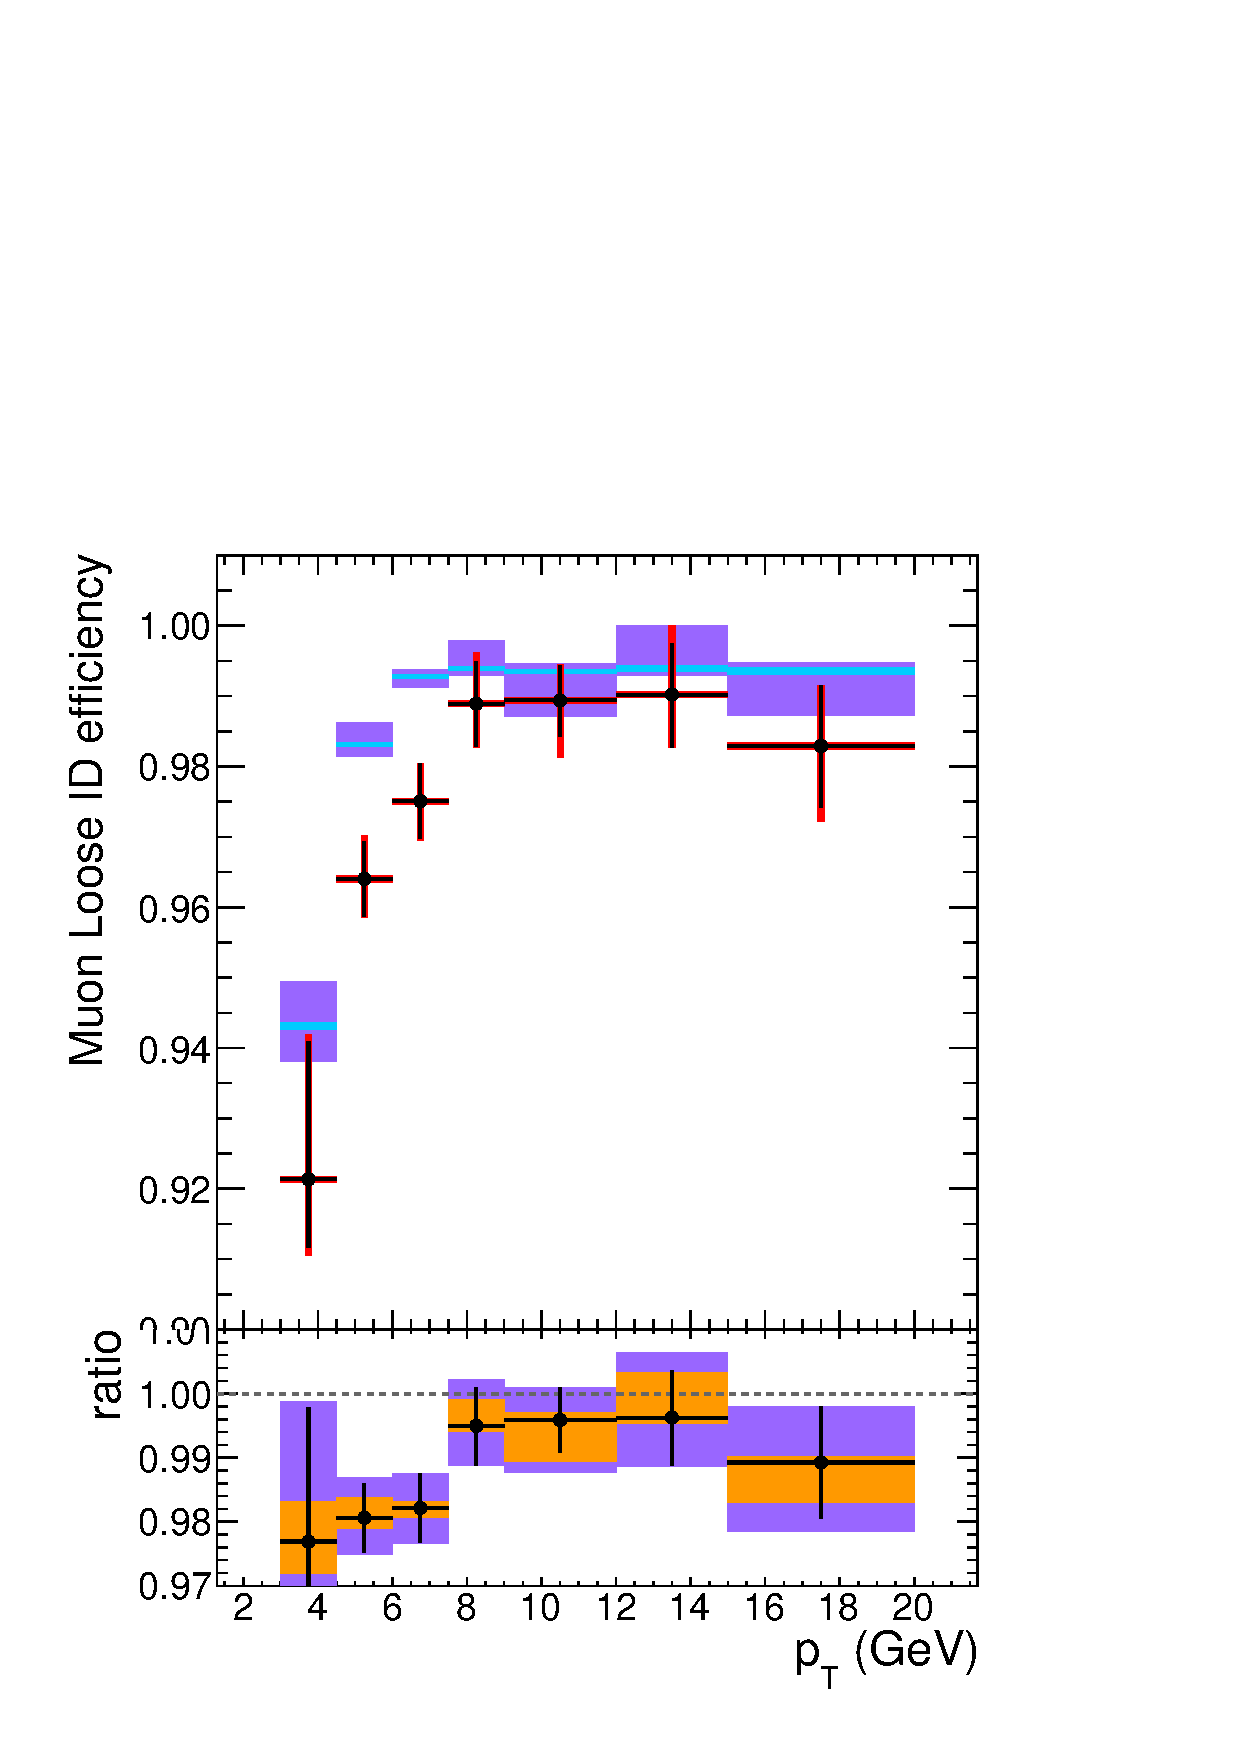
\includegraphics[width=0.30\textwidth]{Figures/Muons/mu_Loose_barrel_2016.pdf}}
    \subfigure[]{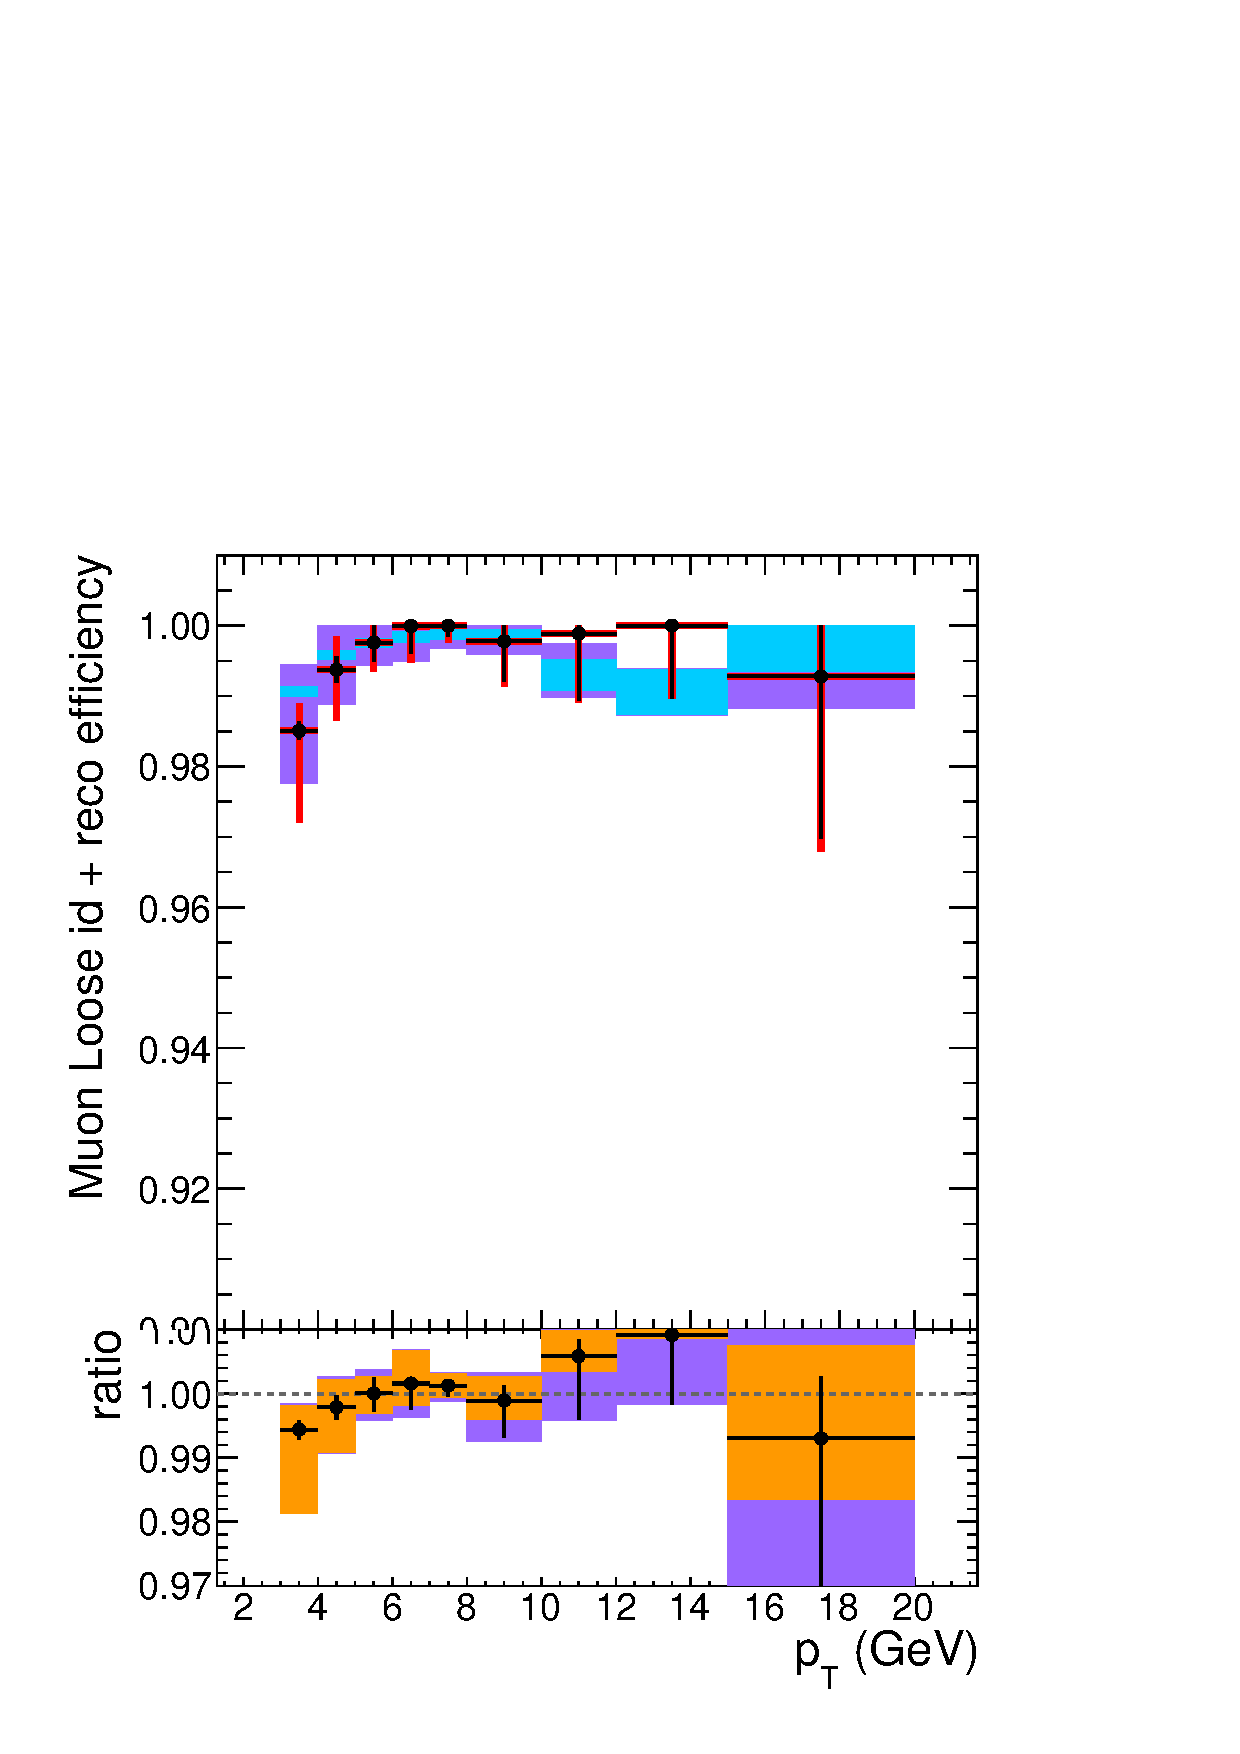
\includegraphics[width=0.30\textwidth]{Figures/Muons/mu_Loose_endcap_2016.pdf}}
    \subfigure[]{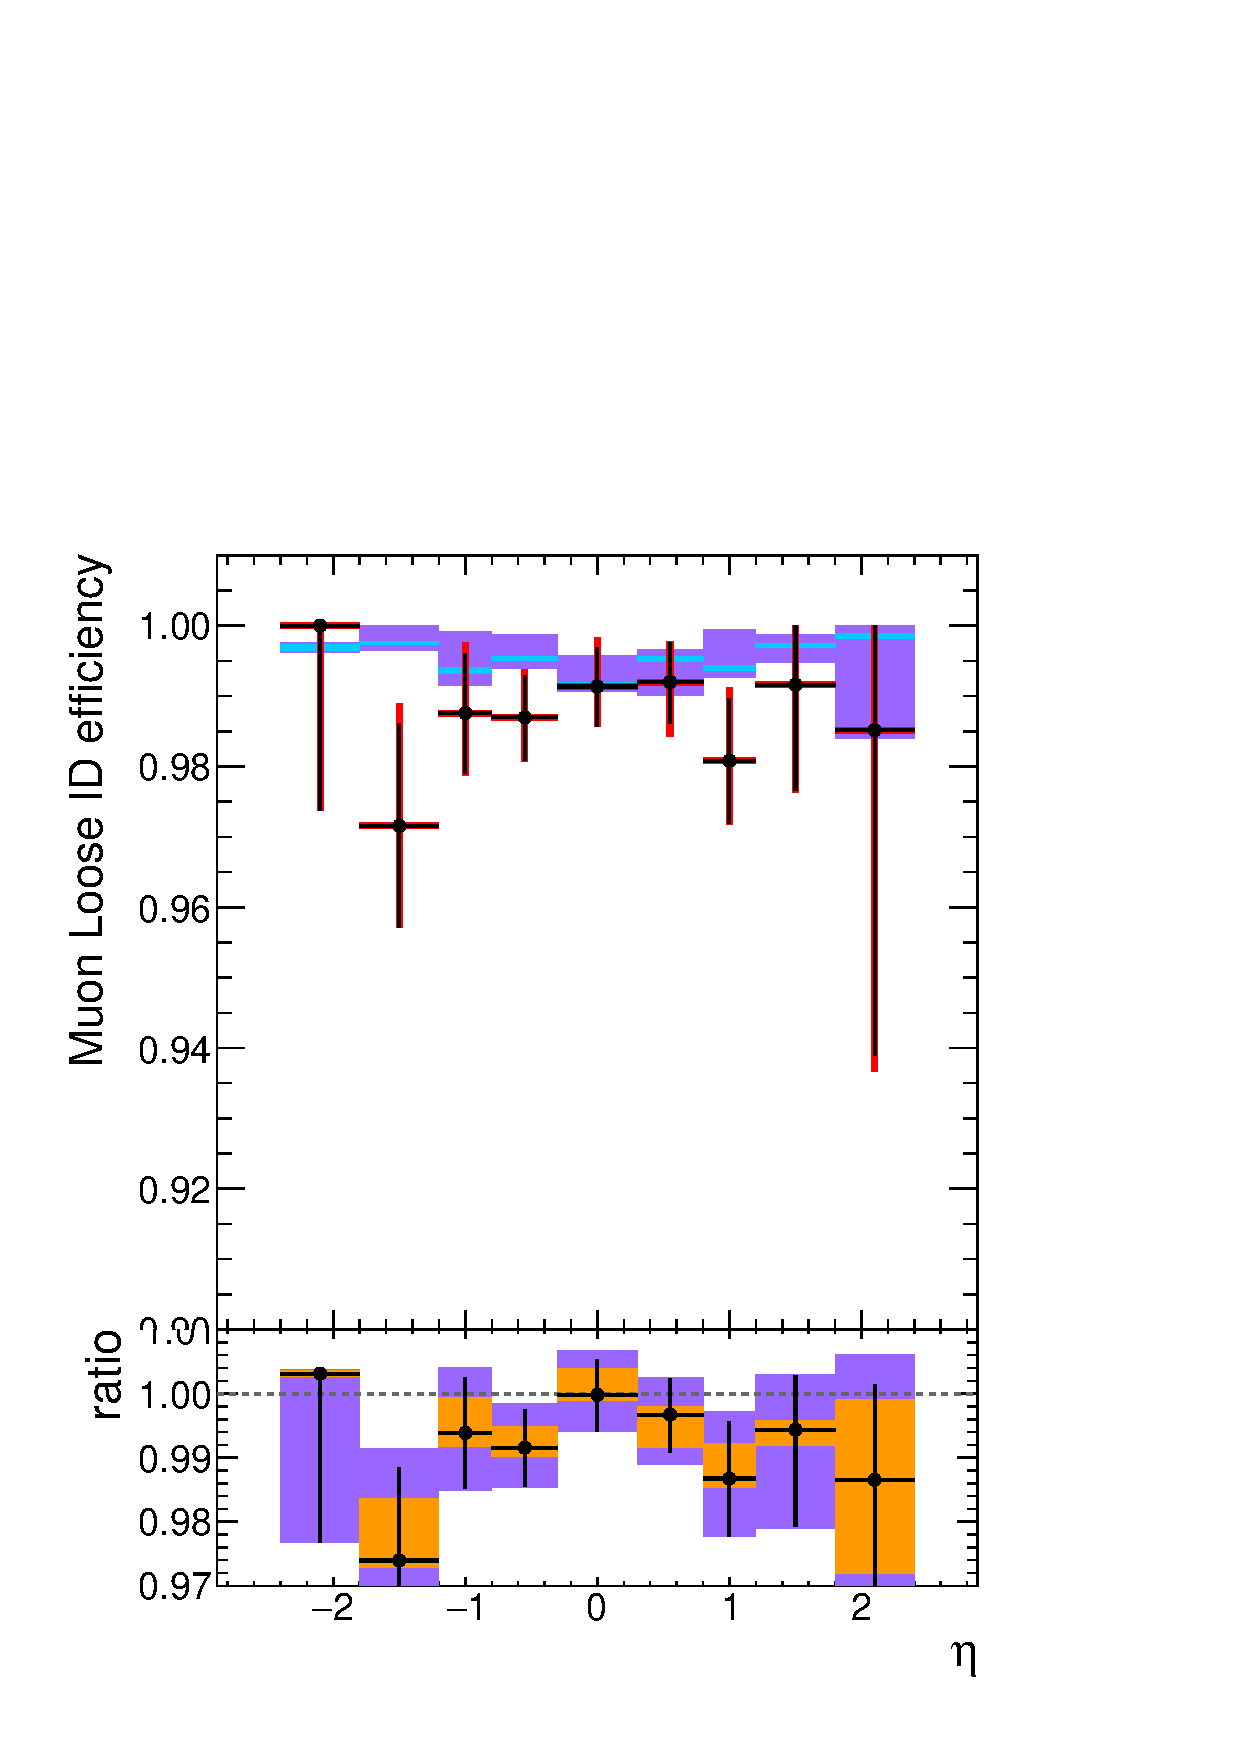
\includegraphics[width=0.30\textwidth]{Figures/Muons/mu_Loose_pt7_2016.pdf}} \\
		\subfigure[]{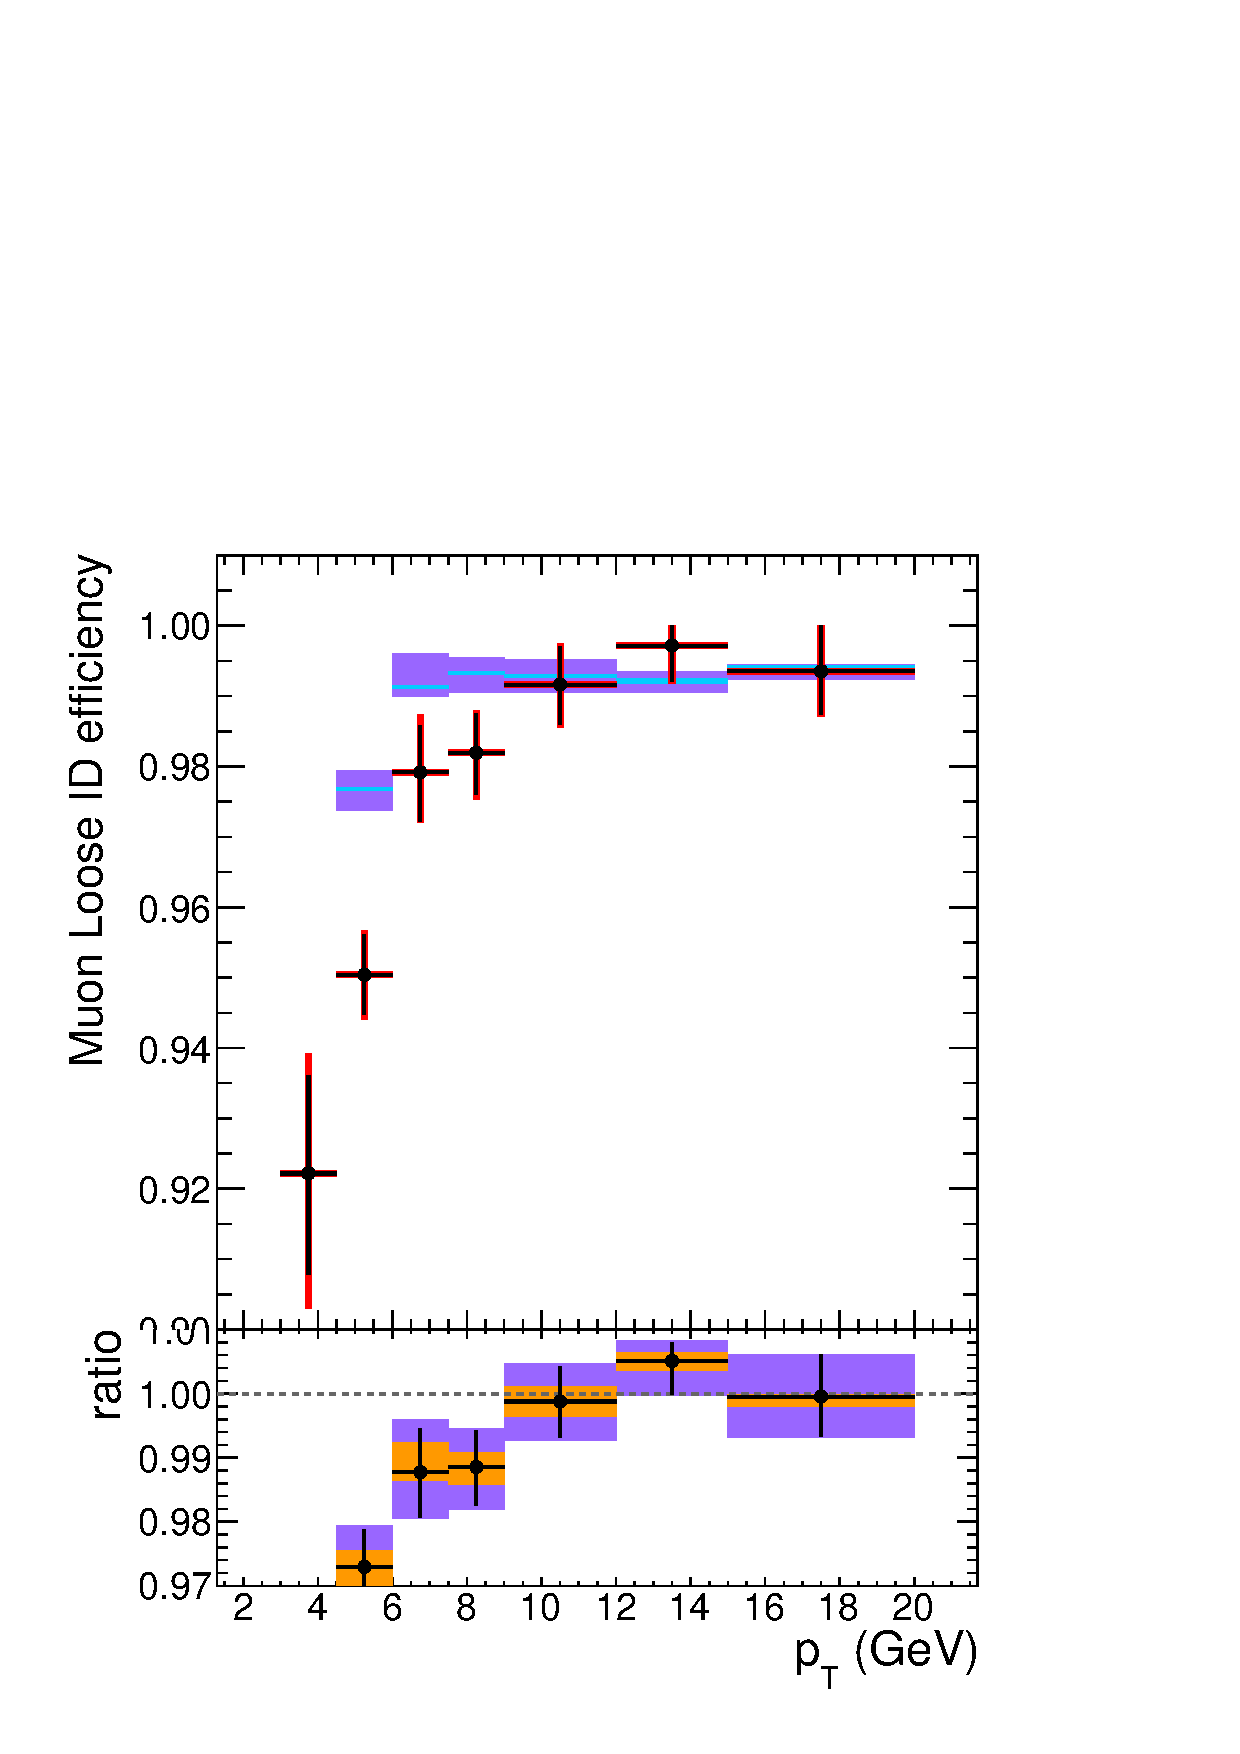
\includegraphics[width=0.30\textwidth]{Figures/Muons/mu_Loose_barrel_2017.pdf}}
    \subfigure[]{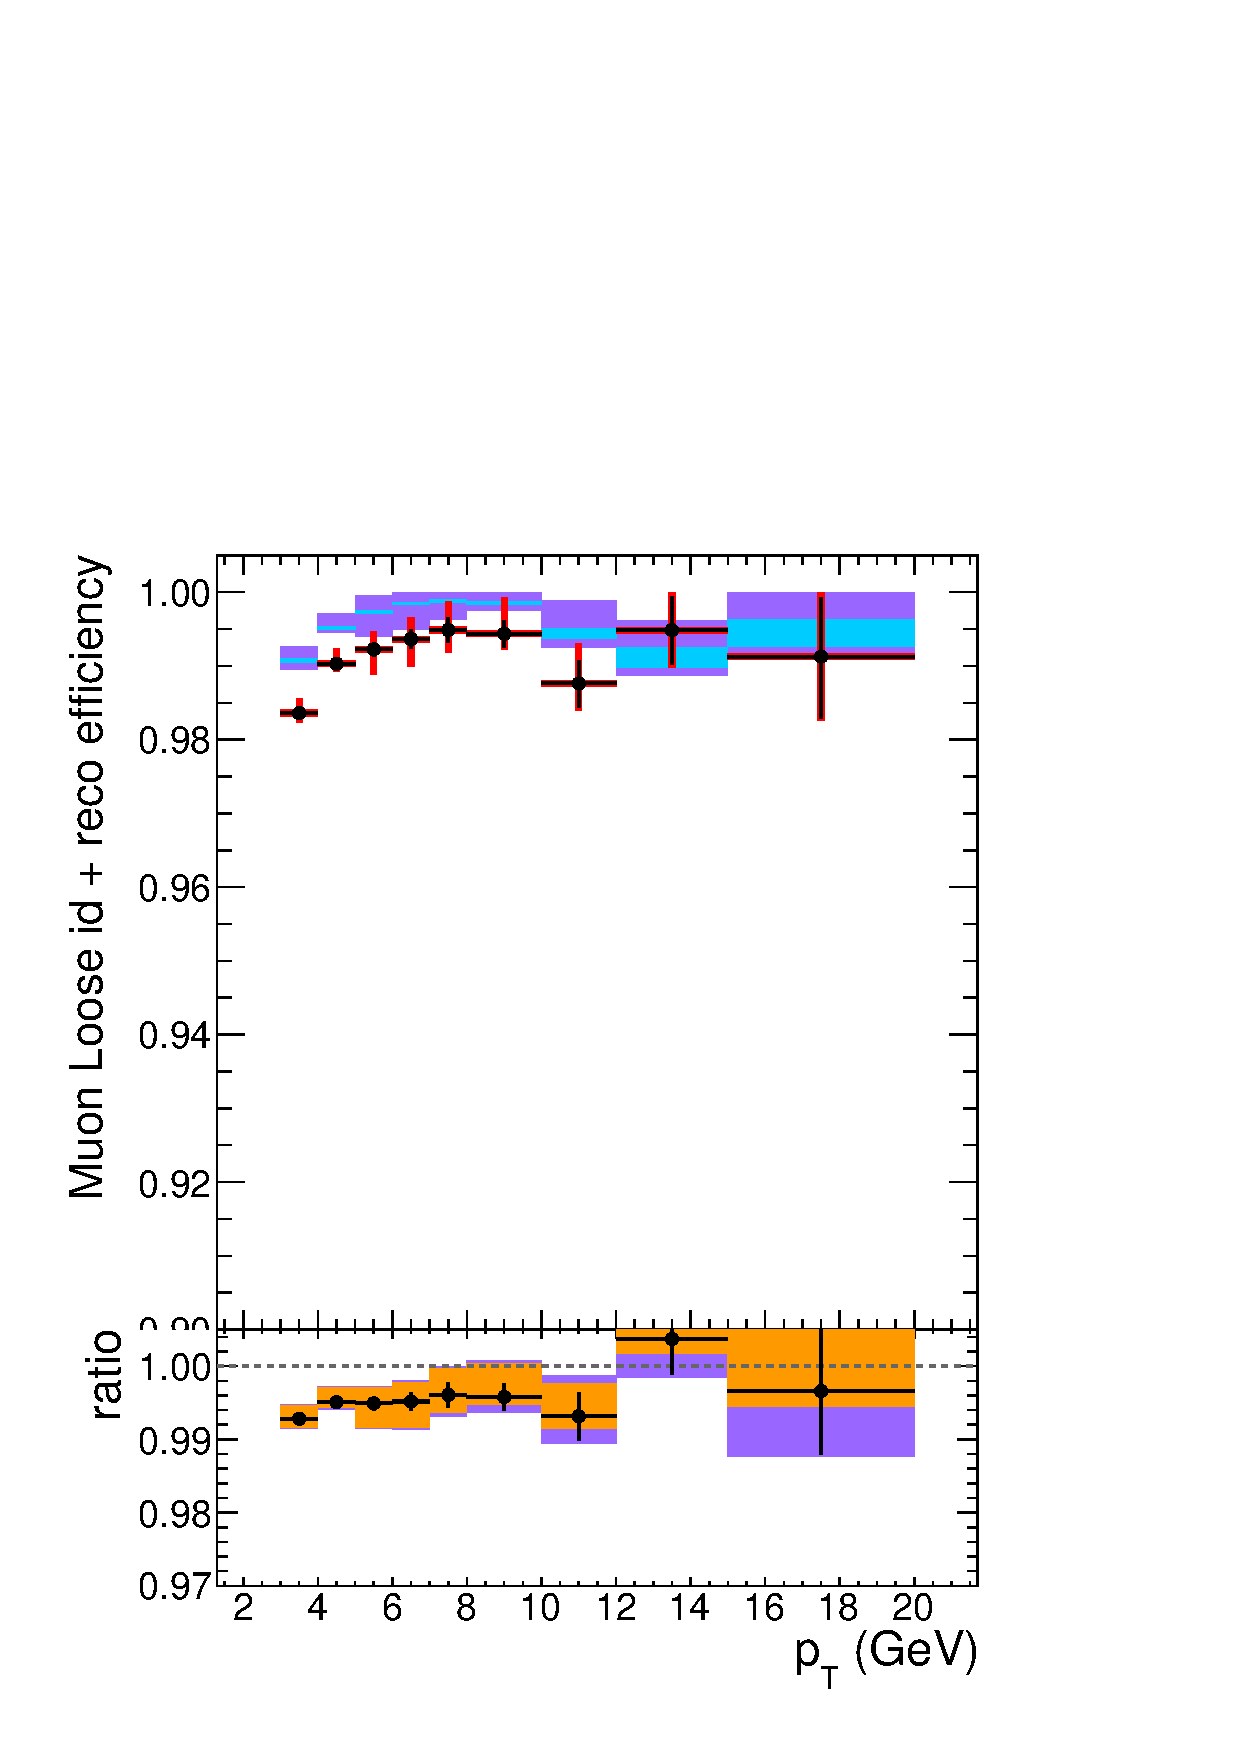
\includegraphics[width=0.30\textwidth]{Figures/Muons/mu_Loose_endcap_2017.pdf}}
    \subfigure[]{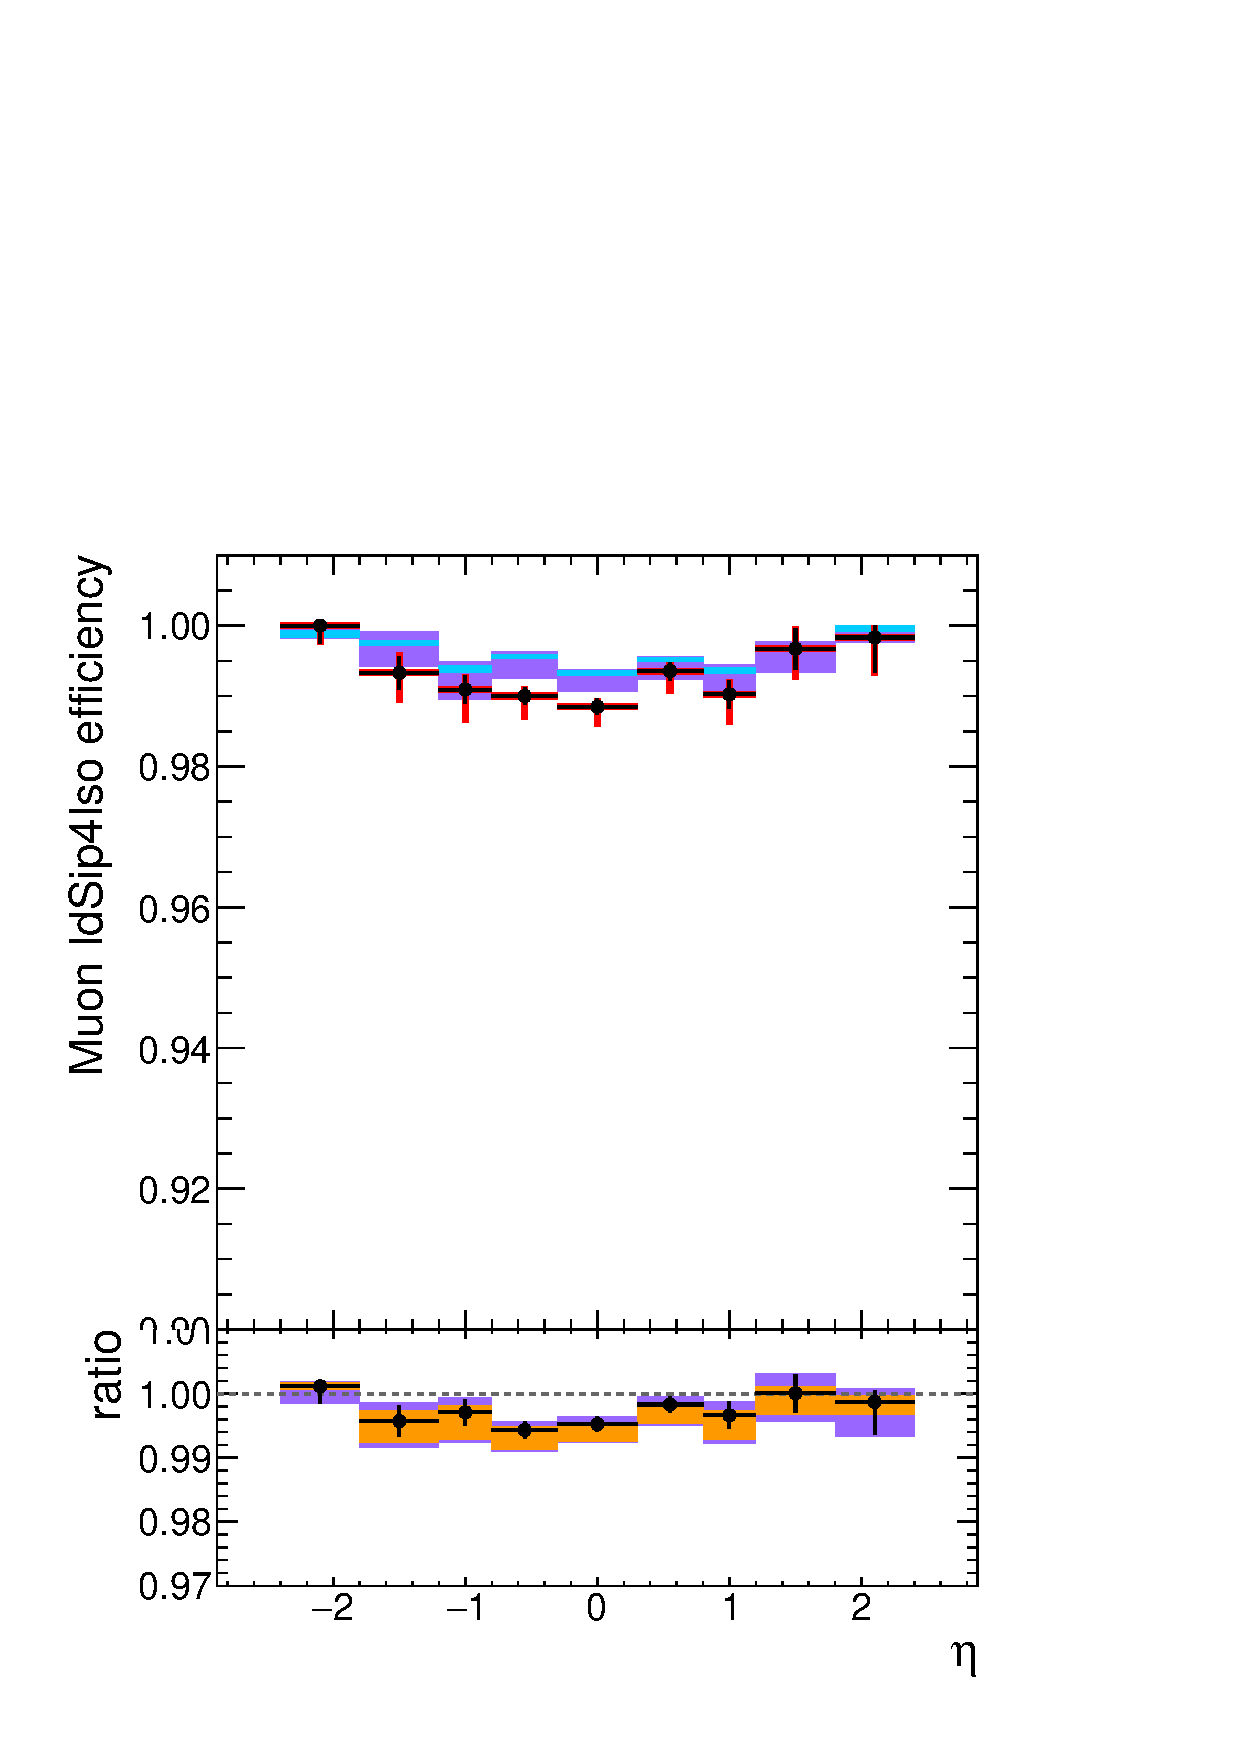
\includegraphics[width=0.30\textwidth]{Figures/Muons/mu_Loose_pt7_2017.pdf}} \\
		\subfigure[]{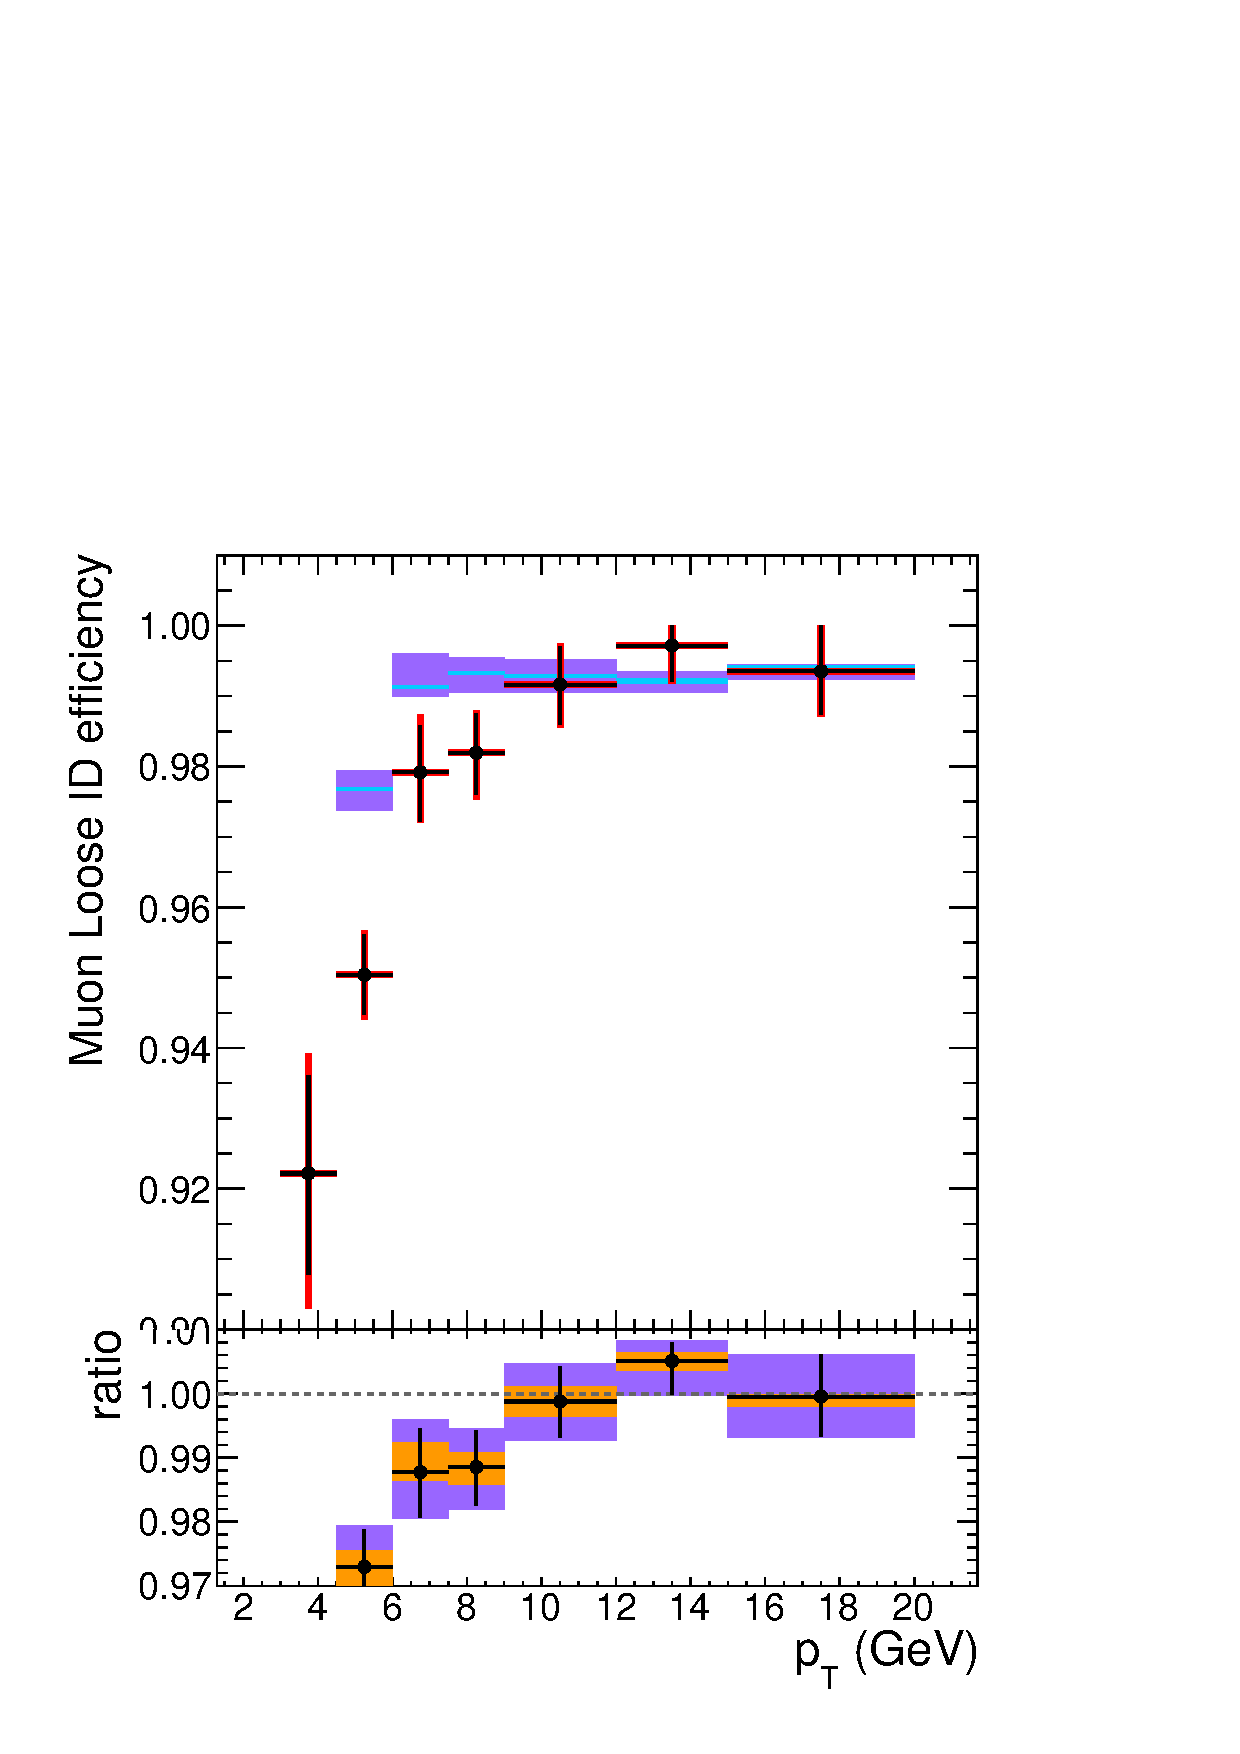
\includegraphics[width=0.30\textwidth]{Figures/Muons/mu_Loose_barrel_2018.pdf}}
    \subfigure[]{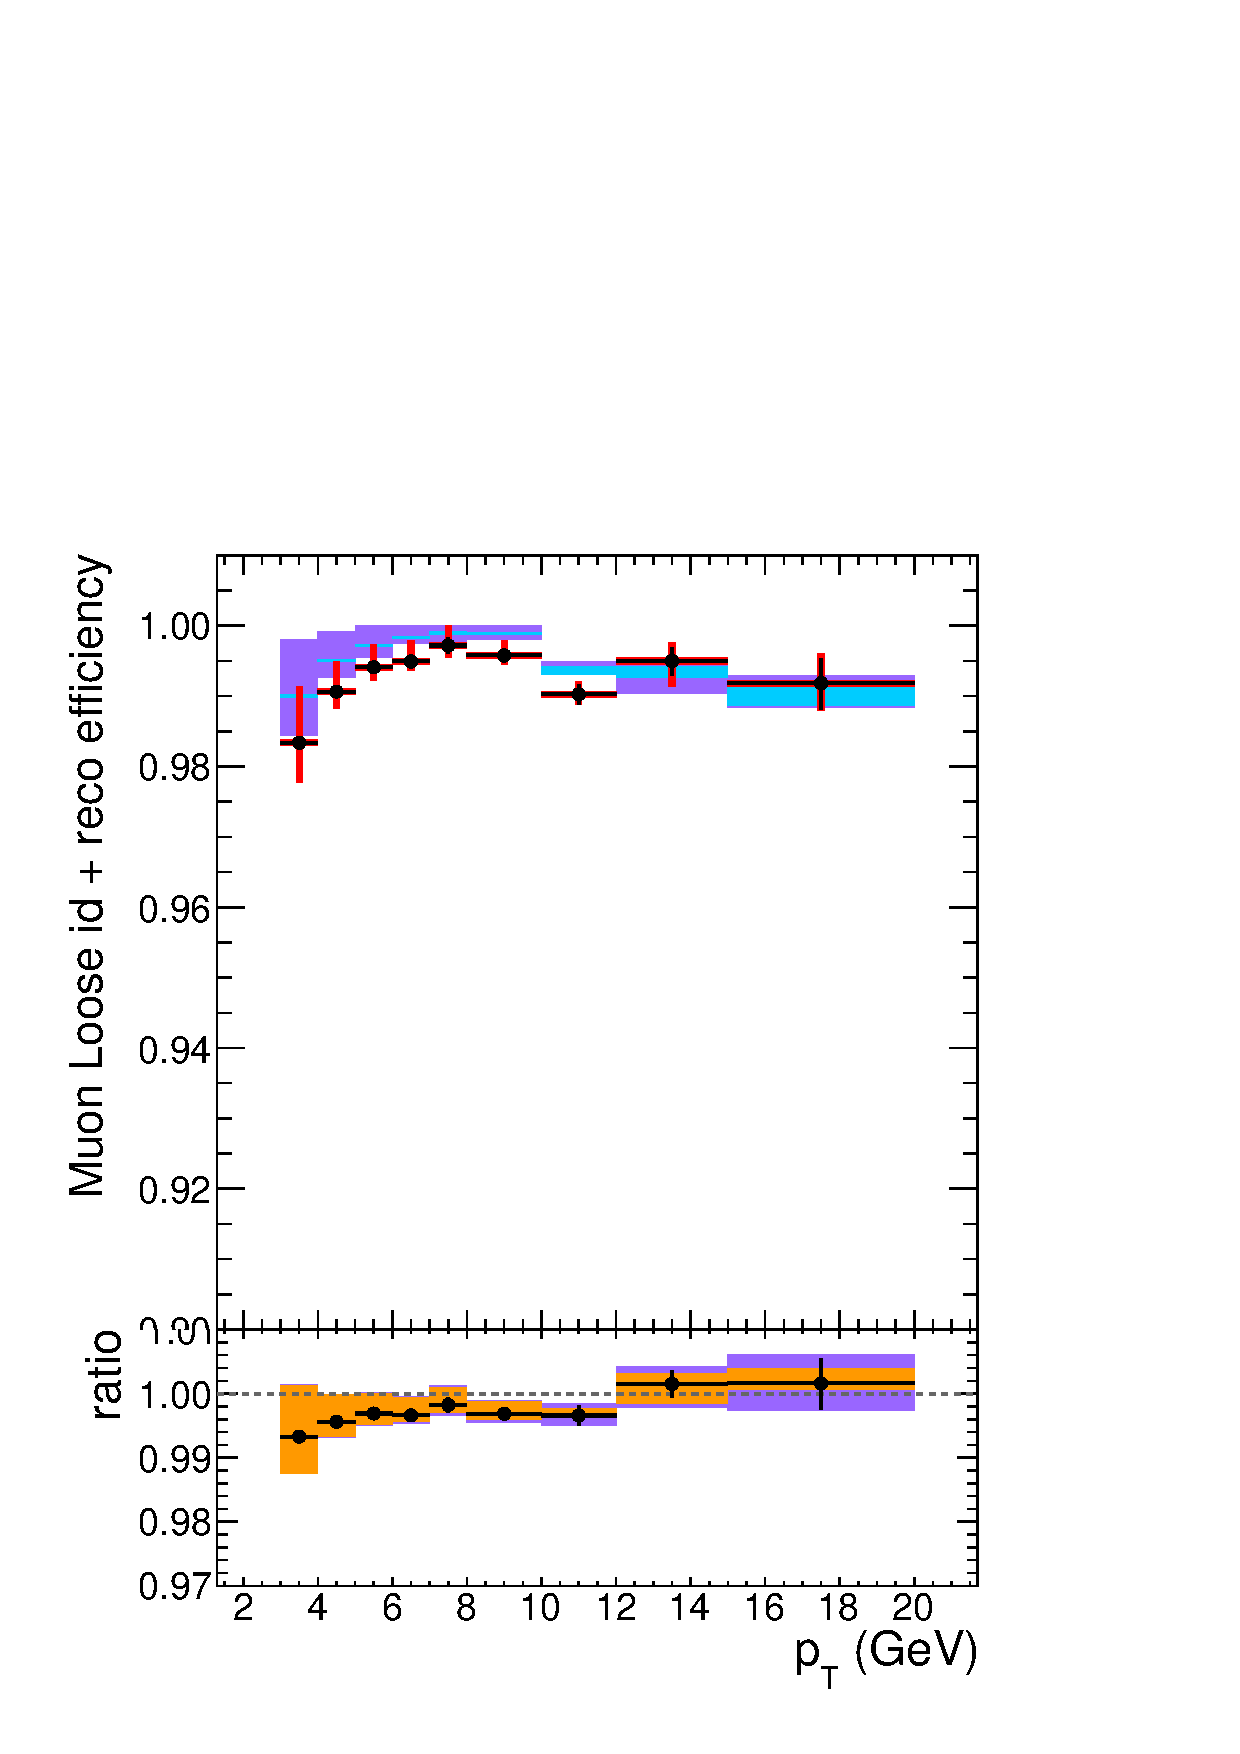
\includegraphics[width=0.30\textwidth]{Figures/Muons/mu_Loose_endcap_2018.pdf}}
    \subfigure[]{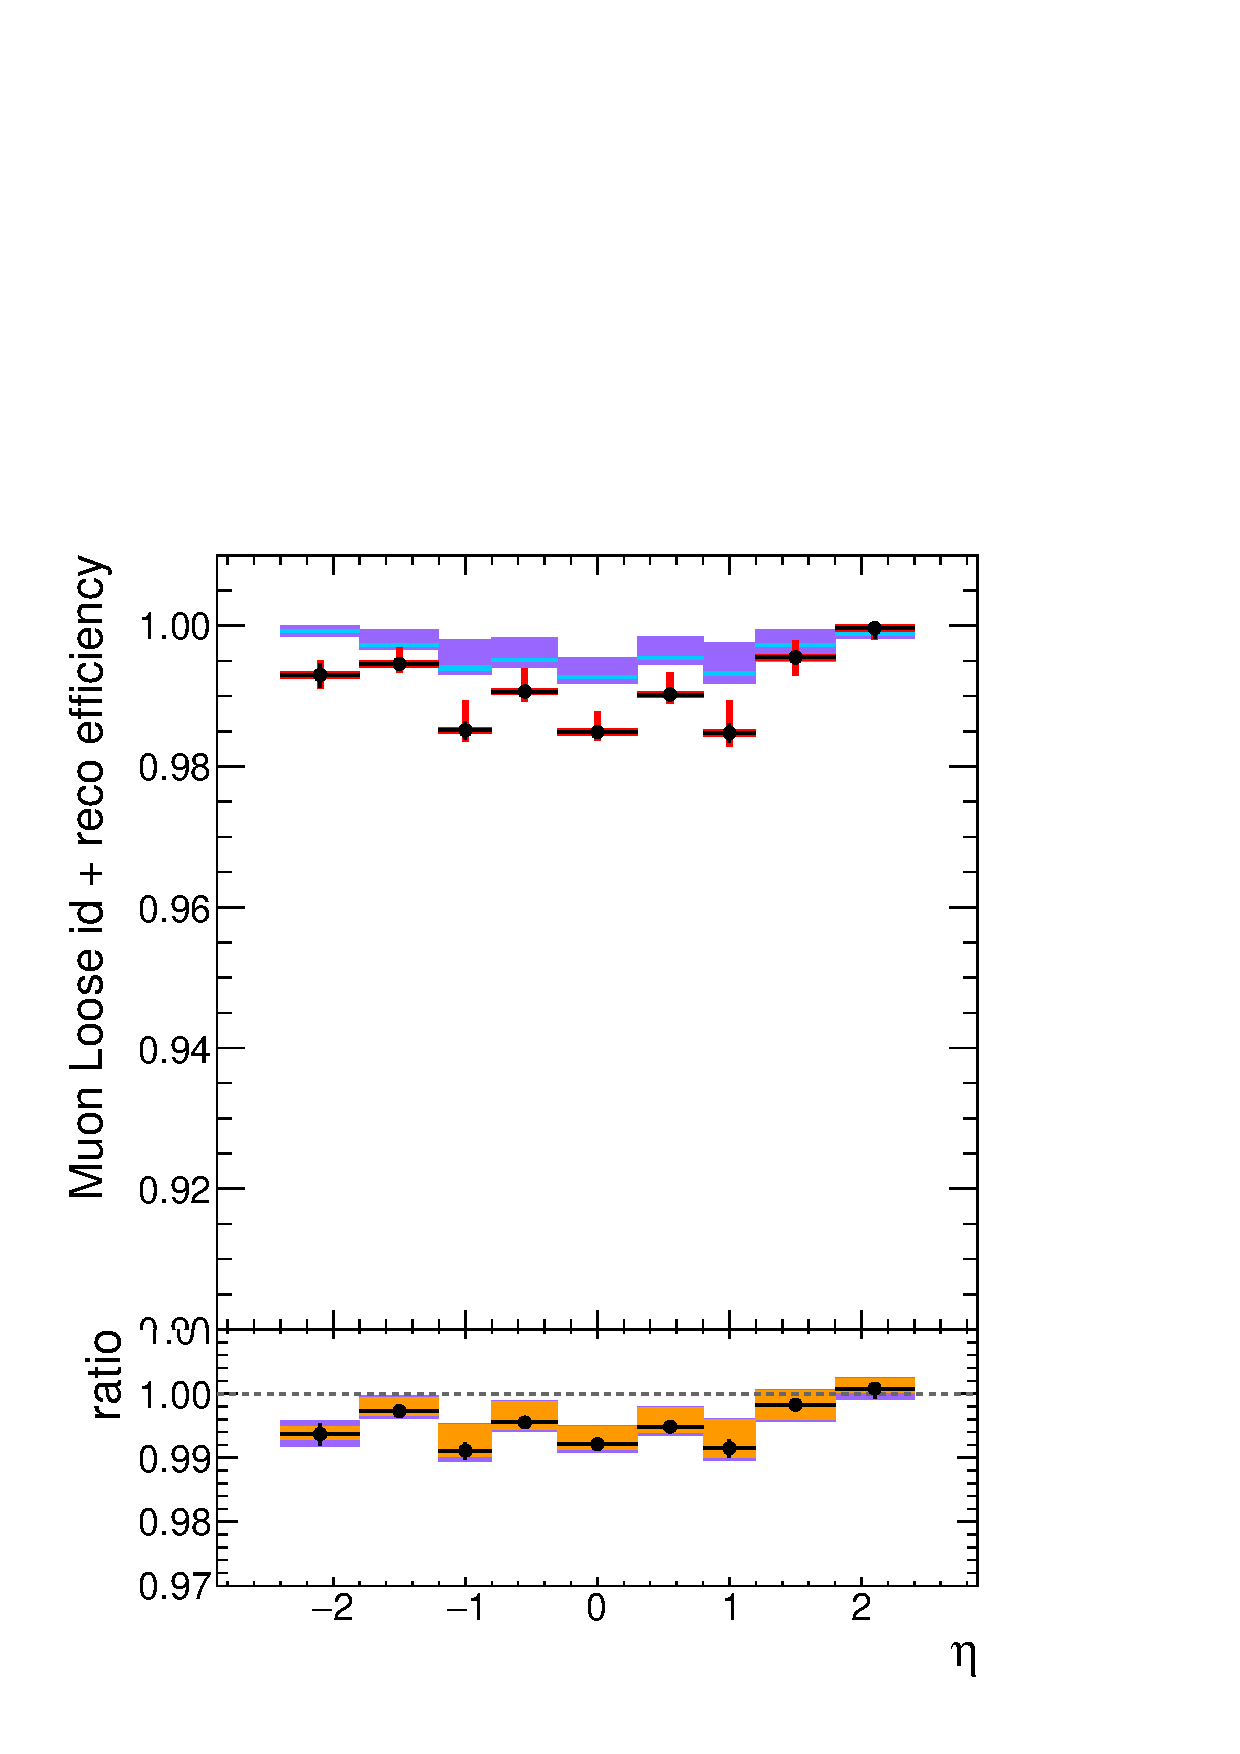
\includegraphics[width=0.30\textwidth]{Figures/Muons/mu_Loose_pt7_2018.pdf}} 
    \caption{Muon reconstruction and identification efficiency at low \pt, measured with the tag\&probe method on \JPsi events, as function of \pt in the barrel (left) and endcaps (center), and as function of $\eta$ for $\pt > 7\GeV$ (right), for 2016 (top), 2017 (middle) and 2018 (bottom). In the upper panel, the larger error bars include also the systematical uncertainties, while the smaller ones are purely statistical. In the lower panel showing the ratio of the two efficiencies, the black error bars are for the statistical uncertainty, the orange rectangles for the systematical uncertainty and the violet rectangles include both uncertainties.}
    \label{fig:MuonIDEff_1}
\end{center}
\end{figure}

\paragraph*{Impact parameter requirements}
%The measurement is performed using $\Z$ events. Events are selected with \verb=HLT_IsoMu27_v*= or \verb=HLT_Mu50_v*= triggers.
The measurement is performed using $\Z$ events. Events are selected with \verb=HLT_IsoMu20_v*= or \verb=HLT_IsoMu22_v*= or \verb=HLT_IsoMu22_eta2p1_v*= for 2016, \verb=HLT_IsoMu27_v*= for 2017 and \verb=HLT_IsoMu24_v*= for 2018 measurements.
For this measurement, the probe is a muon passing the POG Loose identification criteria,
and it is considered a passing probe if it satisfies the SIP3D, dxy, dz cuts of this analysis.
%
The results are shown in Fig.~\ref{fig:MuonIDEff_2}.
%Very good agreement between data and simulation is observed in the barrel (Fig.~\ref{fig:MuonIDEff_2}, left)
%while some inefficiency is visible in the endcaps, especially at large values of $|\eta|$.
%The data to simulation scale factor is found to be flat as function of \pt, so, similarly to what done
%for the identification part, we apply a correction only as function of $\eta$.
\begin{figure}[htbp]
  \begin{center}
    \subfigure[]{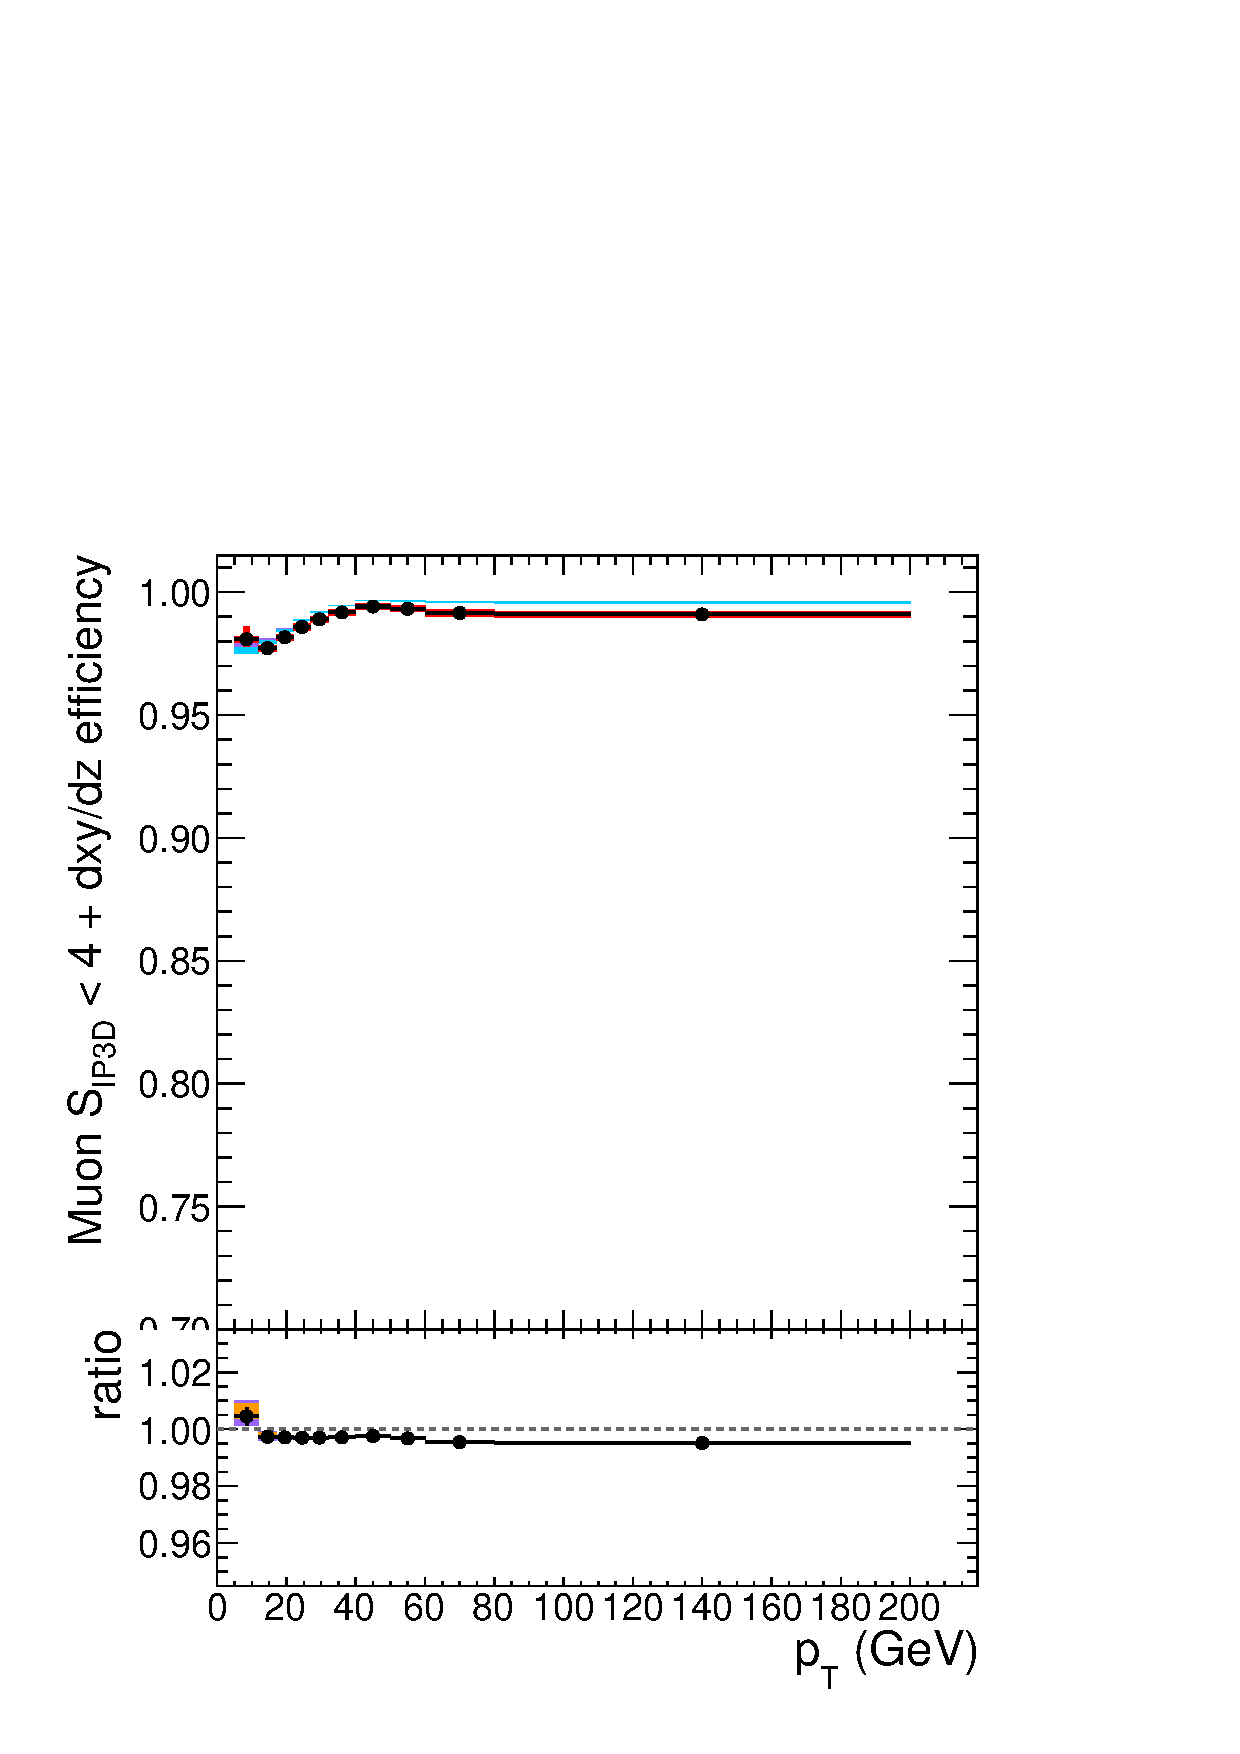
\includegraphics[width=0.32\textwidth]{Figures/Muons/mu_SIP4_barrel_2016.pdf}}
    \subfigure[]{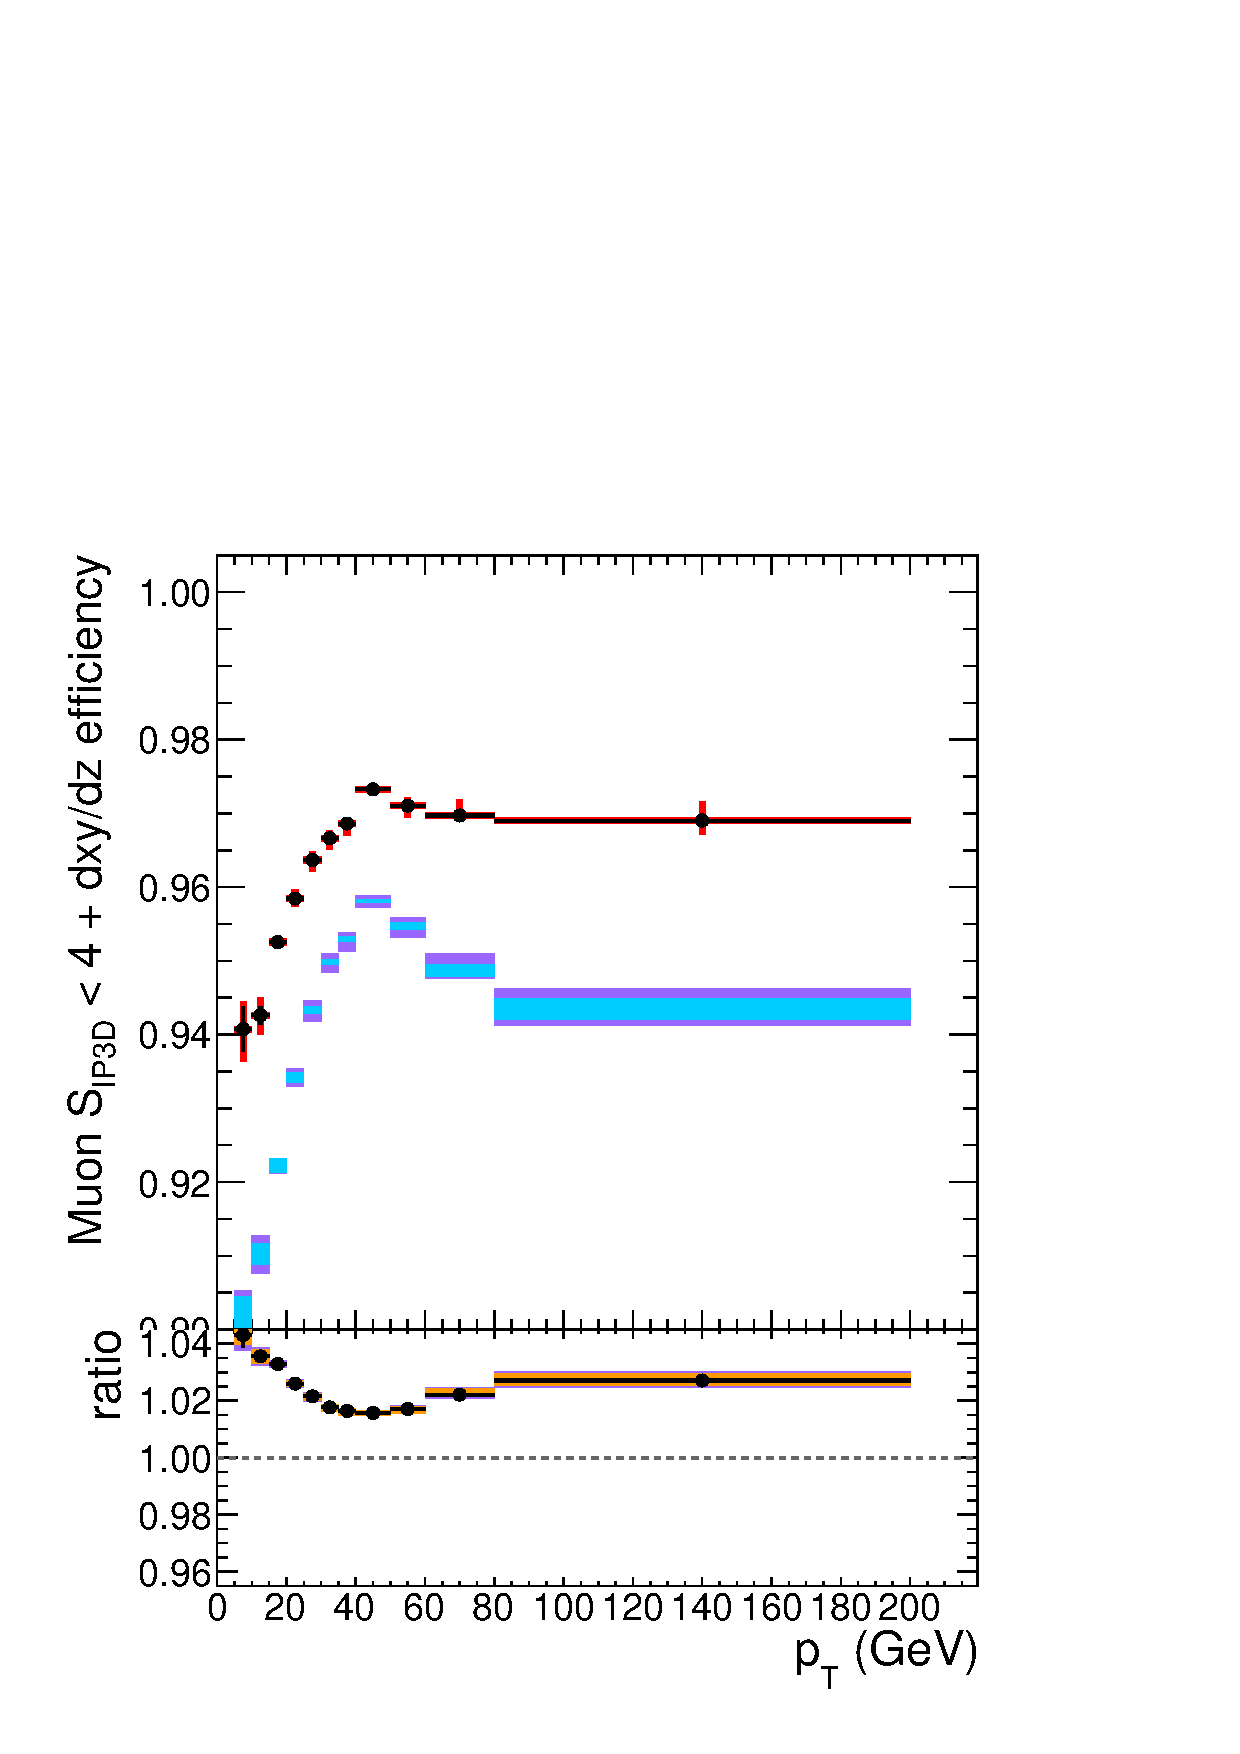
\includegraphics[width=0.32\textwidth]{Figures/Muons/mu_SIP4_endcap_2016.pdf}}
    \subfigure[]{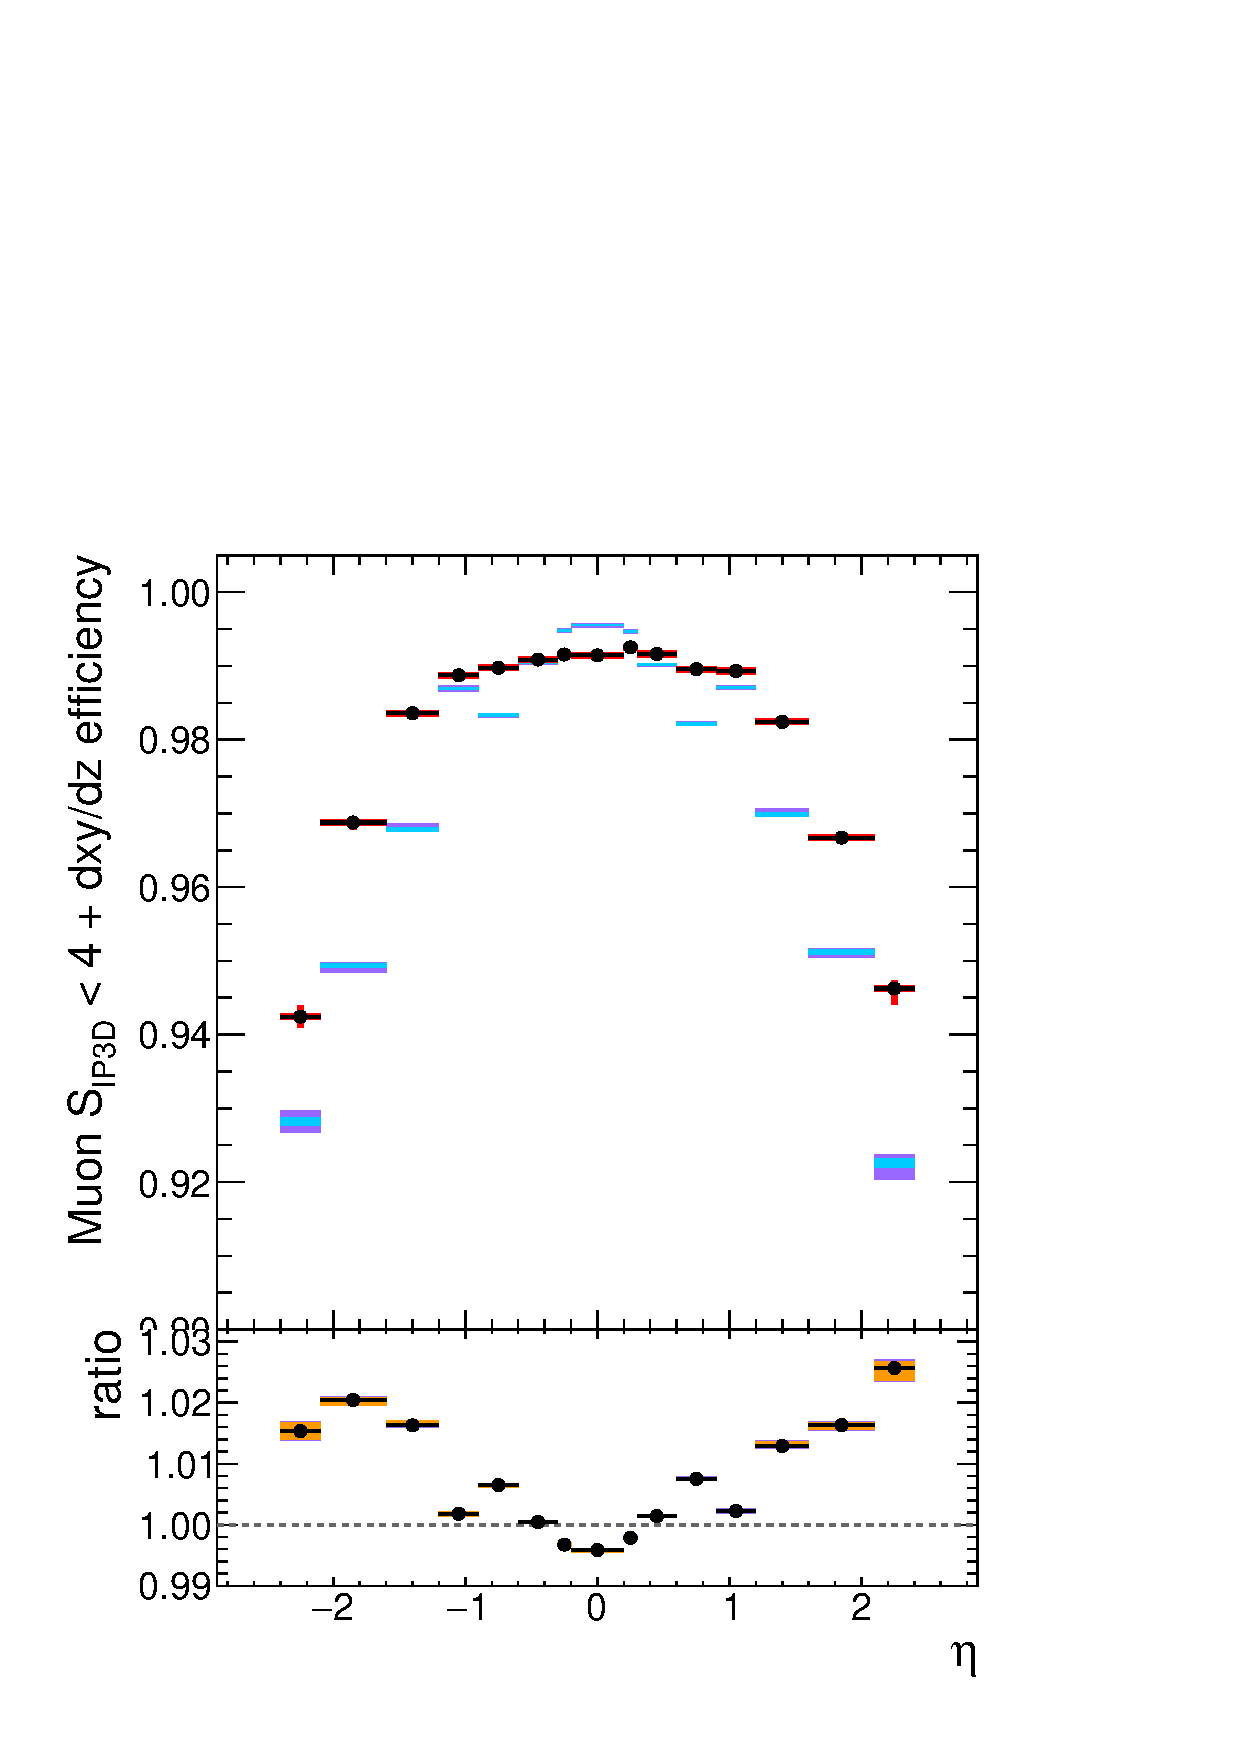
\includegraphics[width=0.32\textwidth]{Figures/Muons/mu_SIP4_pt20_2016.pdf}} \\ 
		\subfigure[]{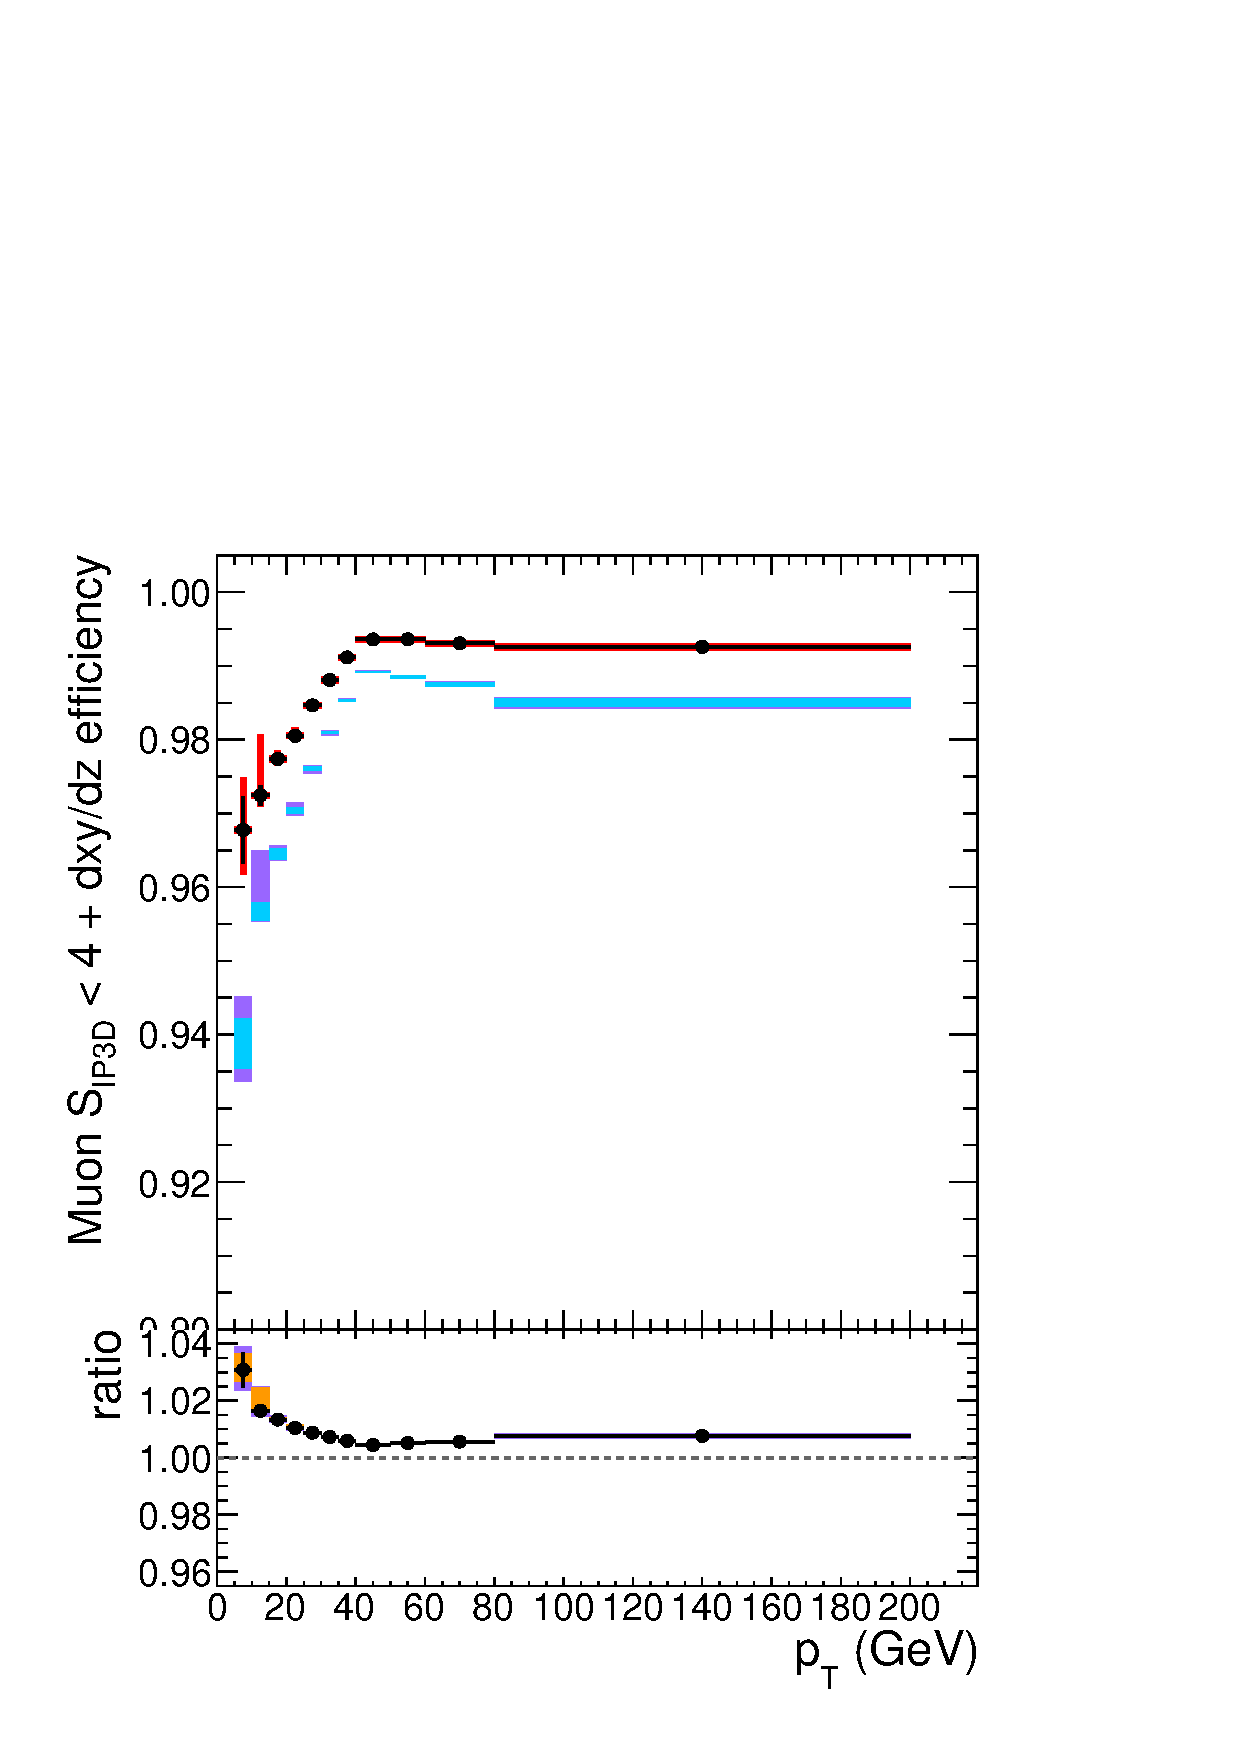
\includegraphics[width=0.32\textwidth]{Figures/Muons/mu_SIP4_barrel_2017.pdf}}
    \subfigure[]{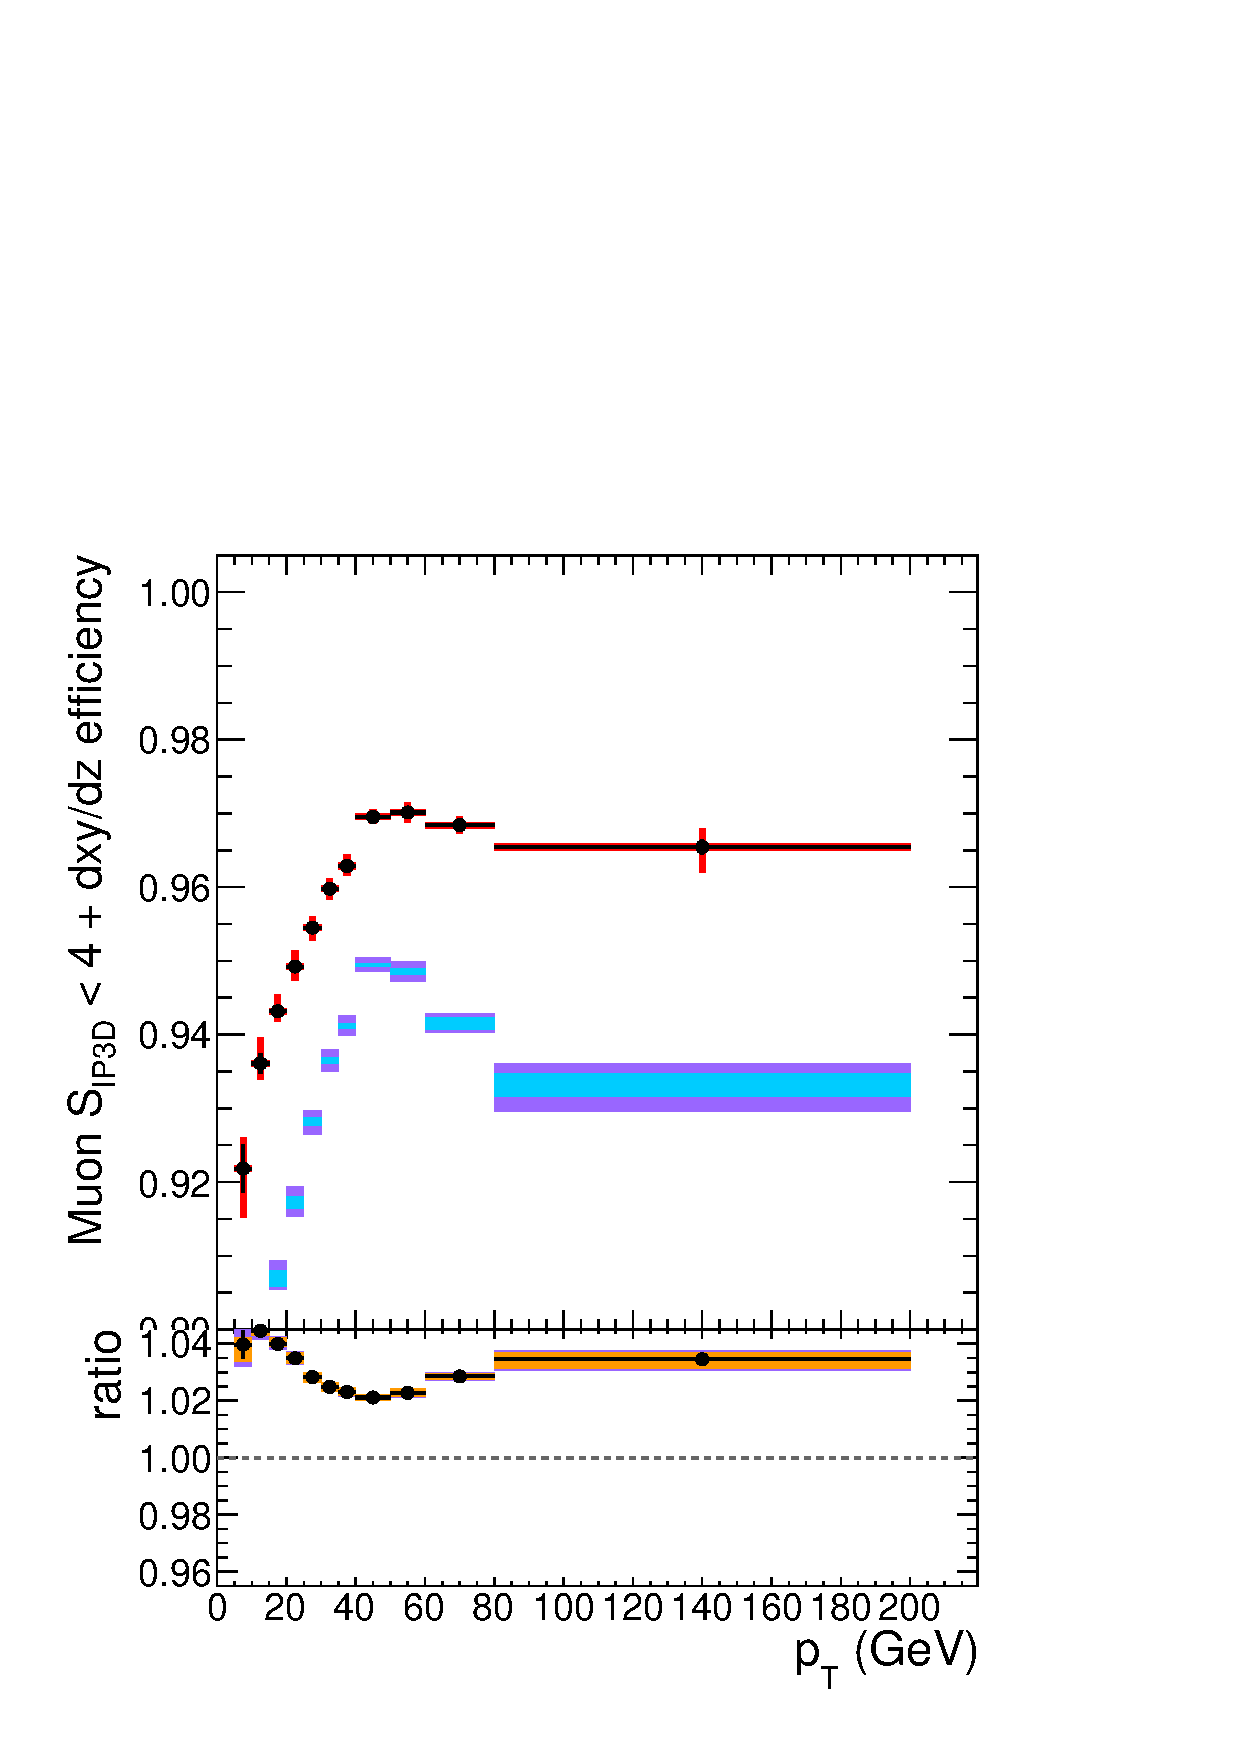
\includegraphics[width=0.32\textwidth]{Figures/Muons/mu_SIP4_endcap_2017.pdf}}
    \subfigure[]{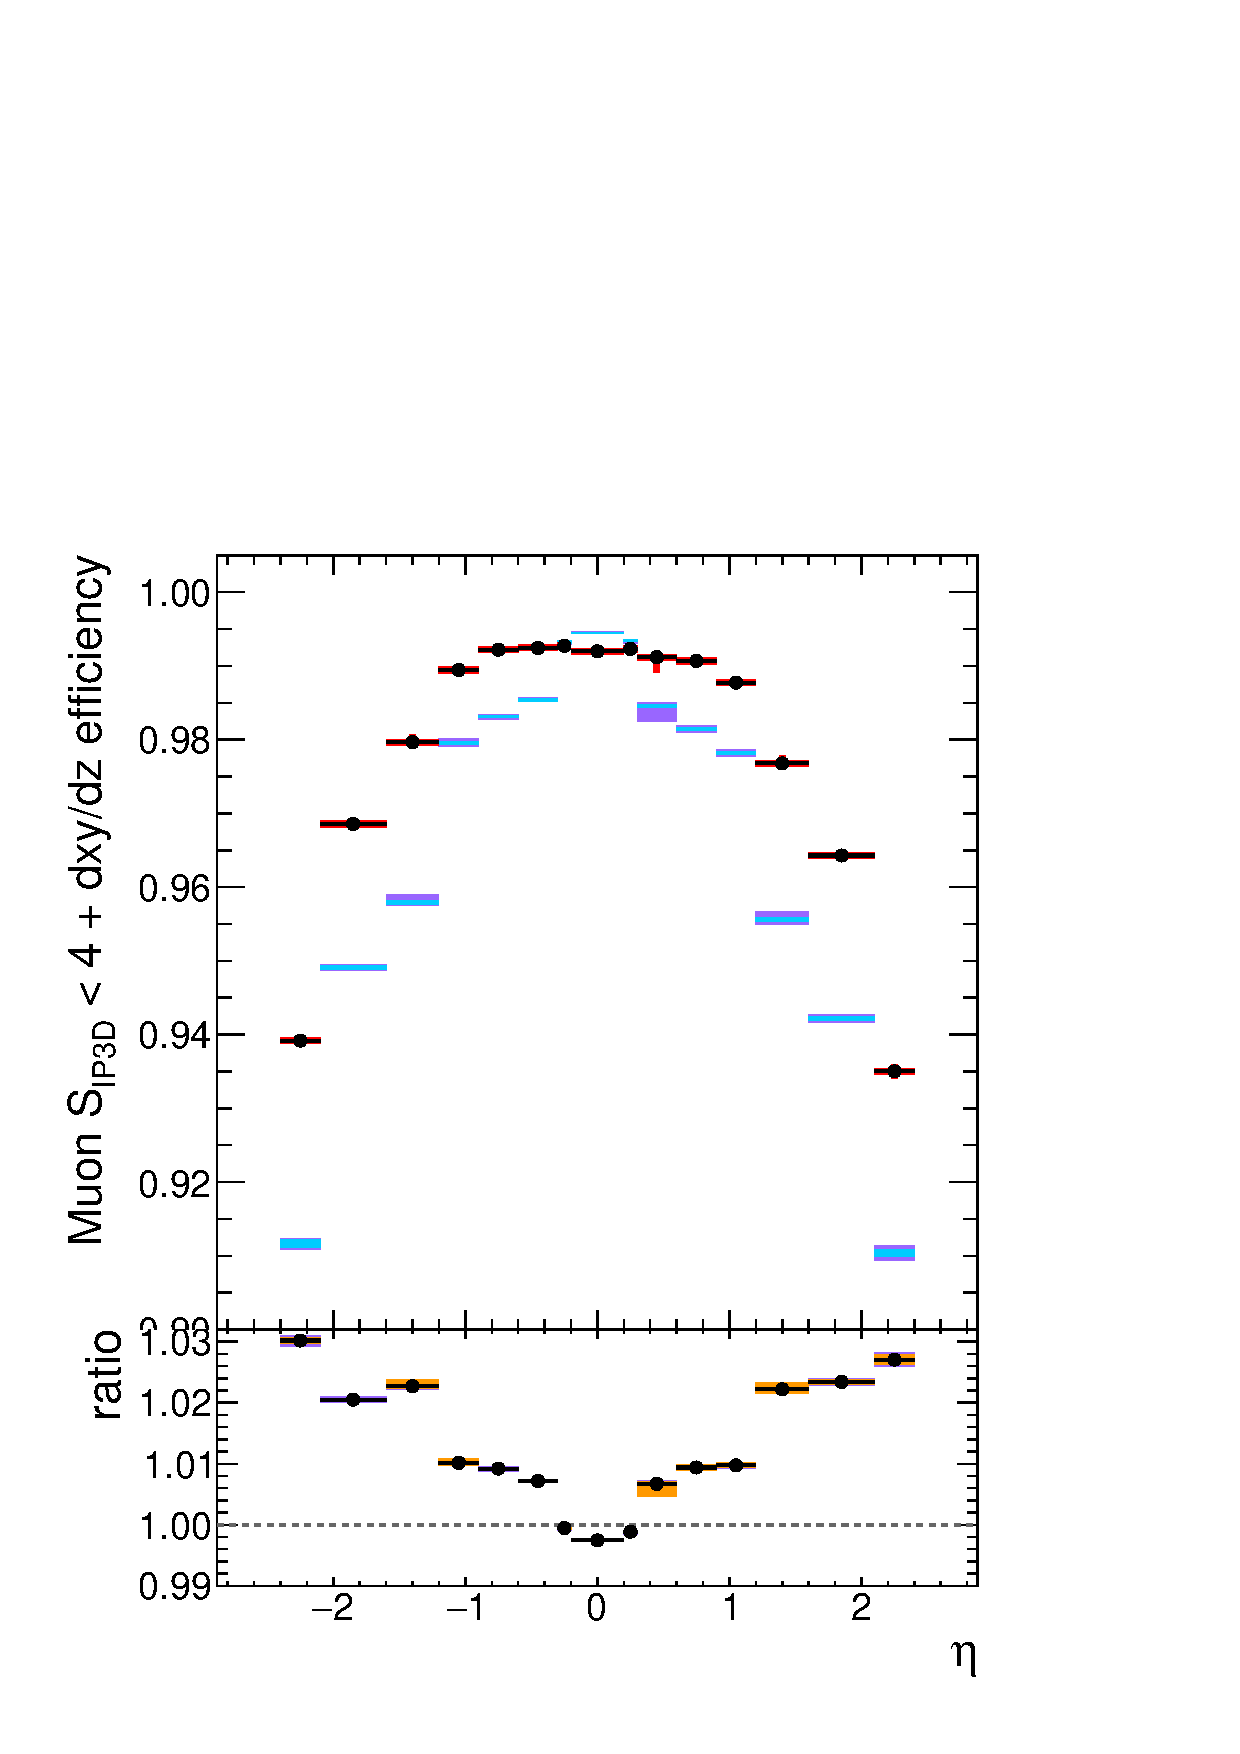
\includegraphics[width=0.32\textwidth]{Figures/Muons/mu_SIP4_pt20_2017.pdf}} \\
		\subfigure[]{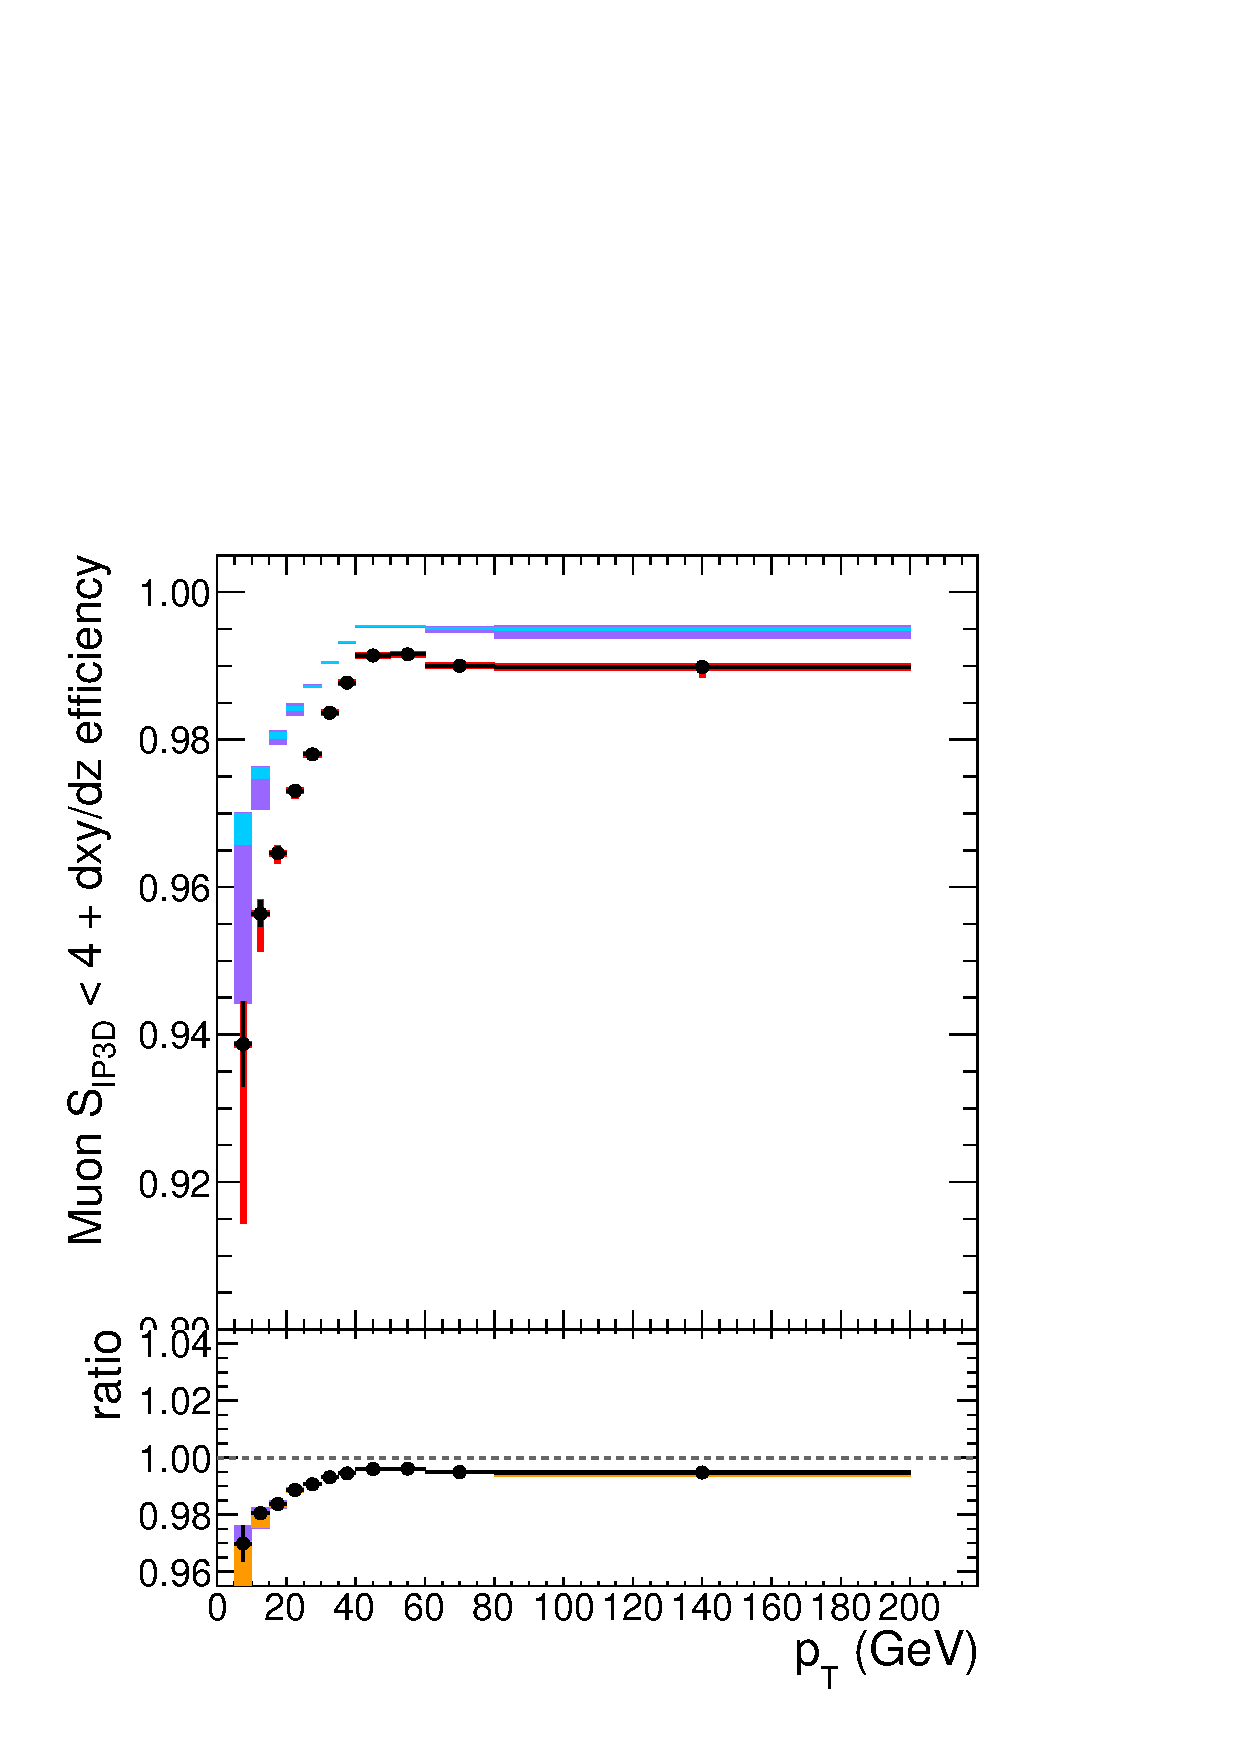
\includegraphics[width=0.32\textwidth]{Figures/Muons/mu_SIP4_barrel_2018.pdf}}
    \subfigure[]{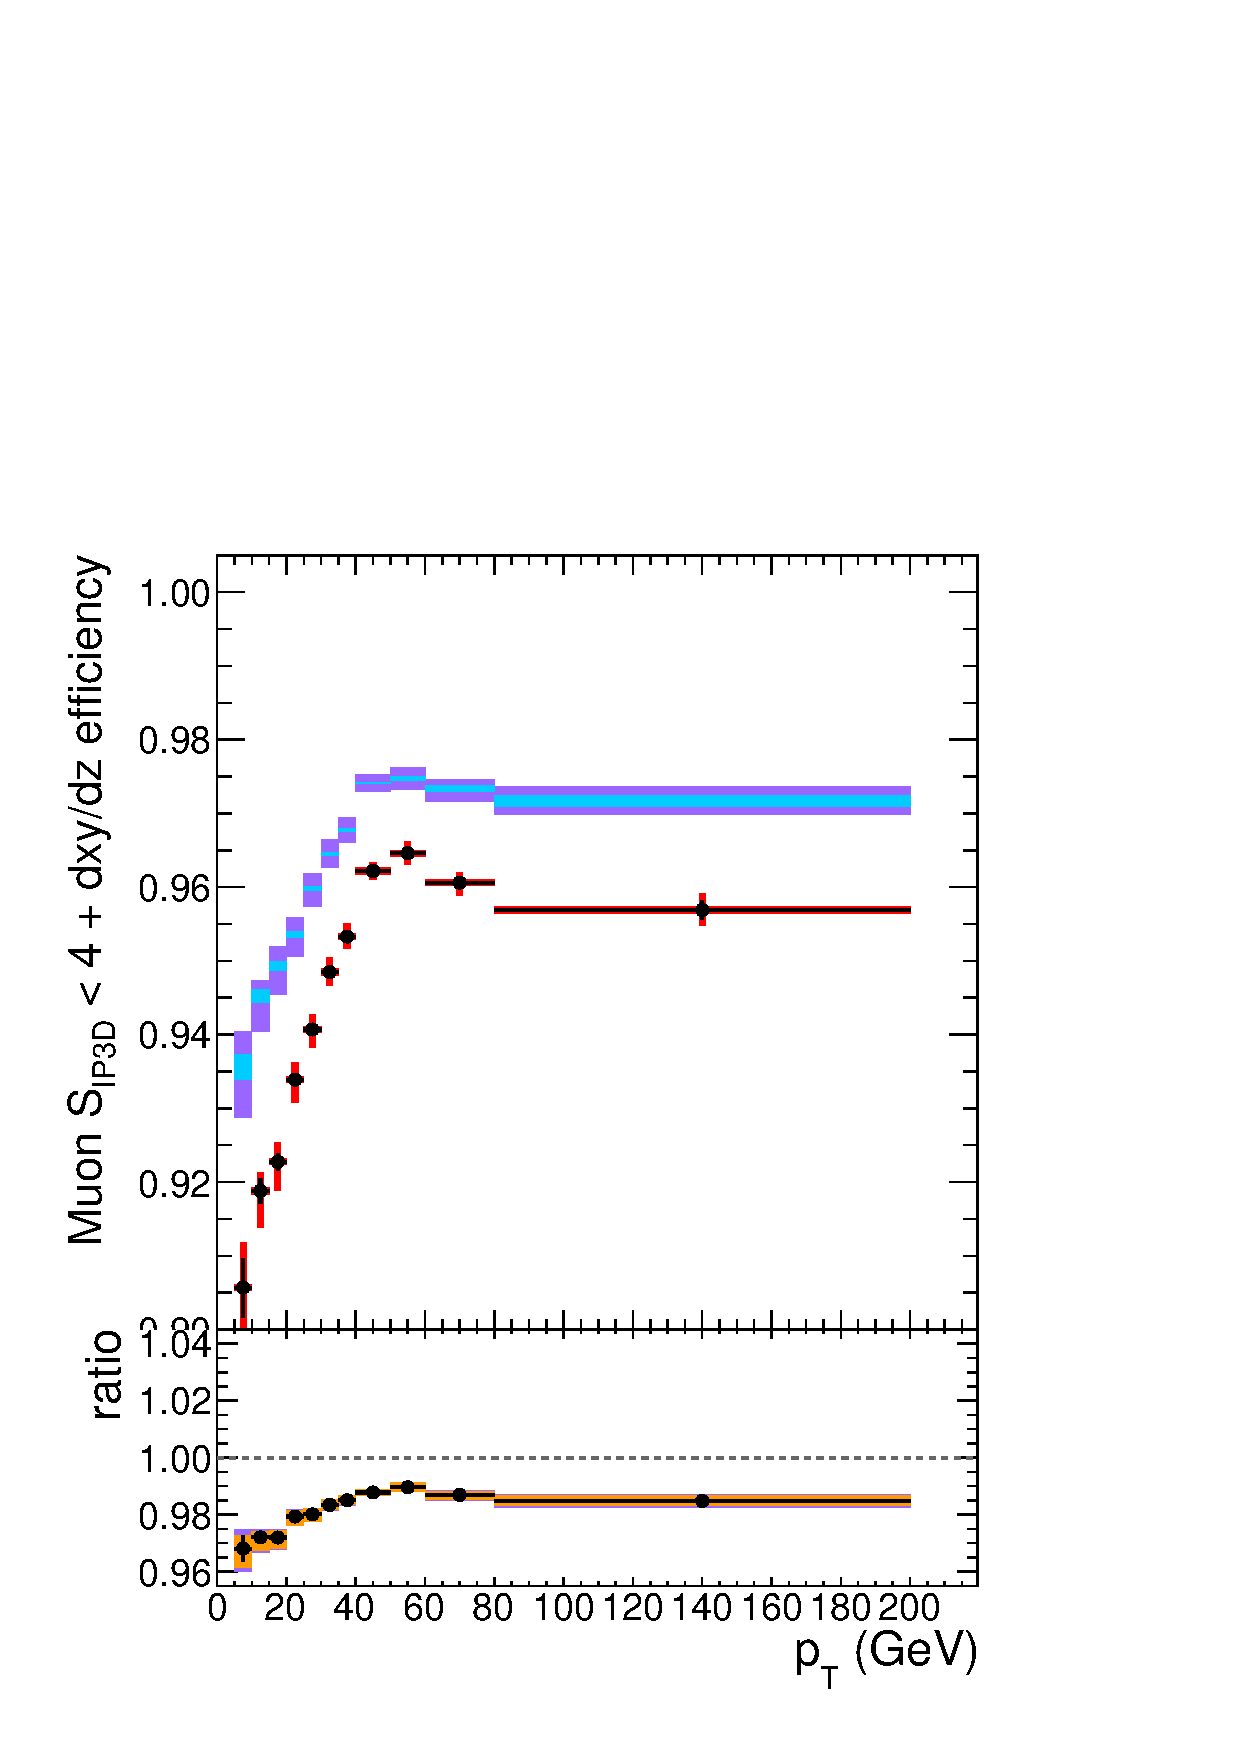
\includegraphics[width=0.32\textwidth]{Figures/Muons/mu_SIP4_endcap_2018.pdf}}
    \subfigure[]{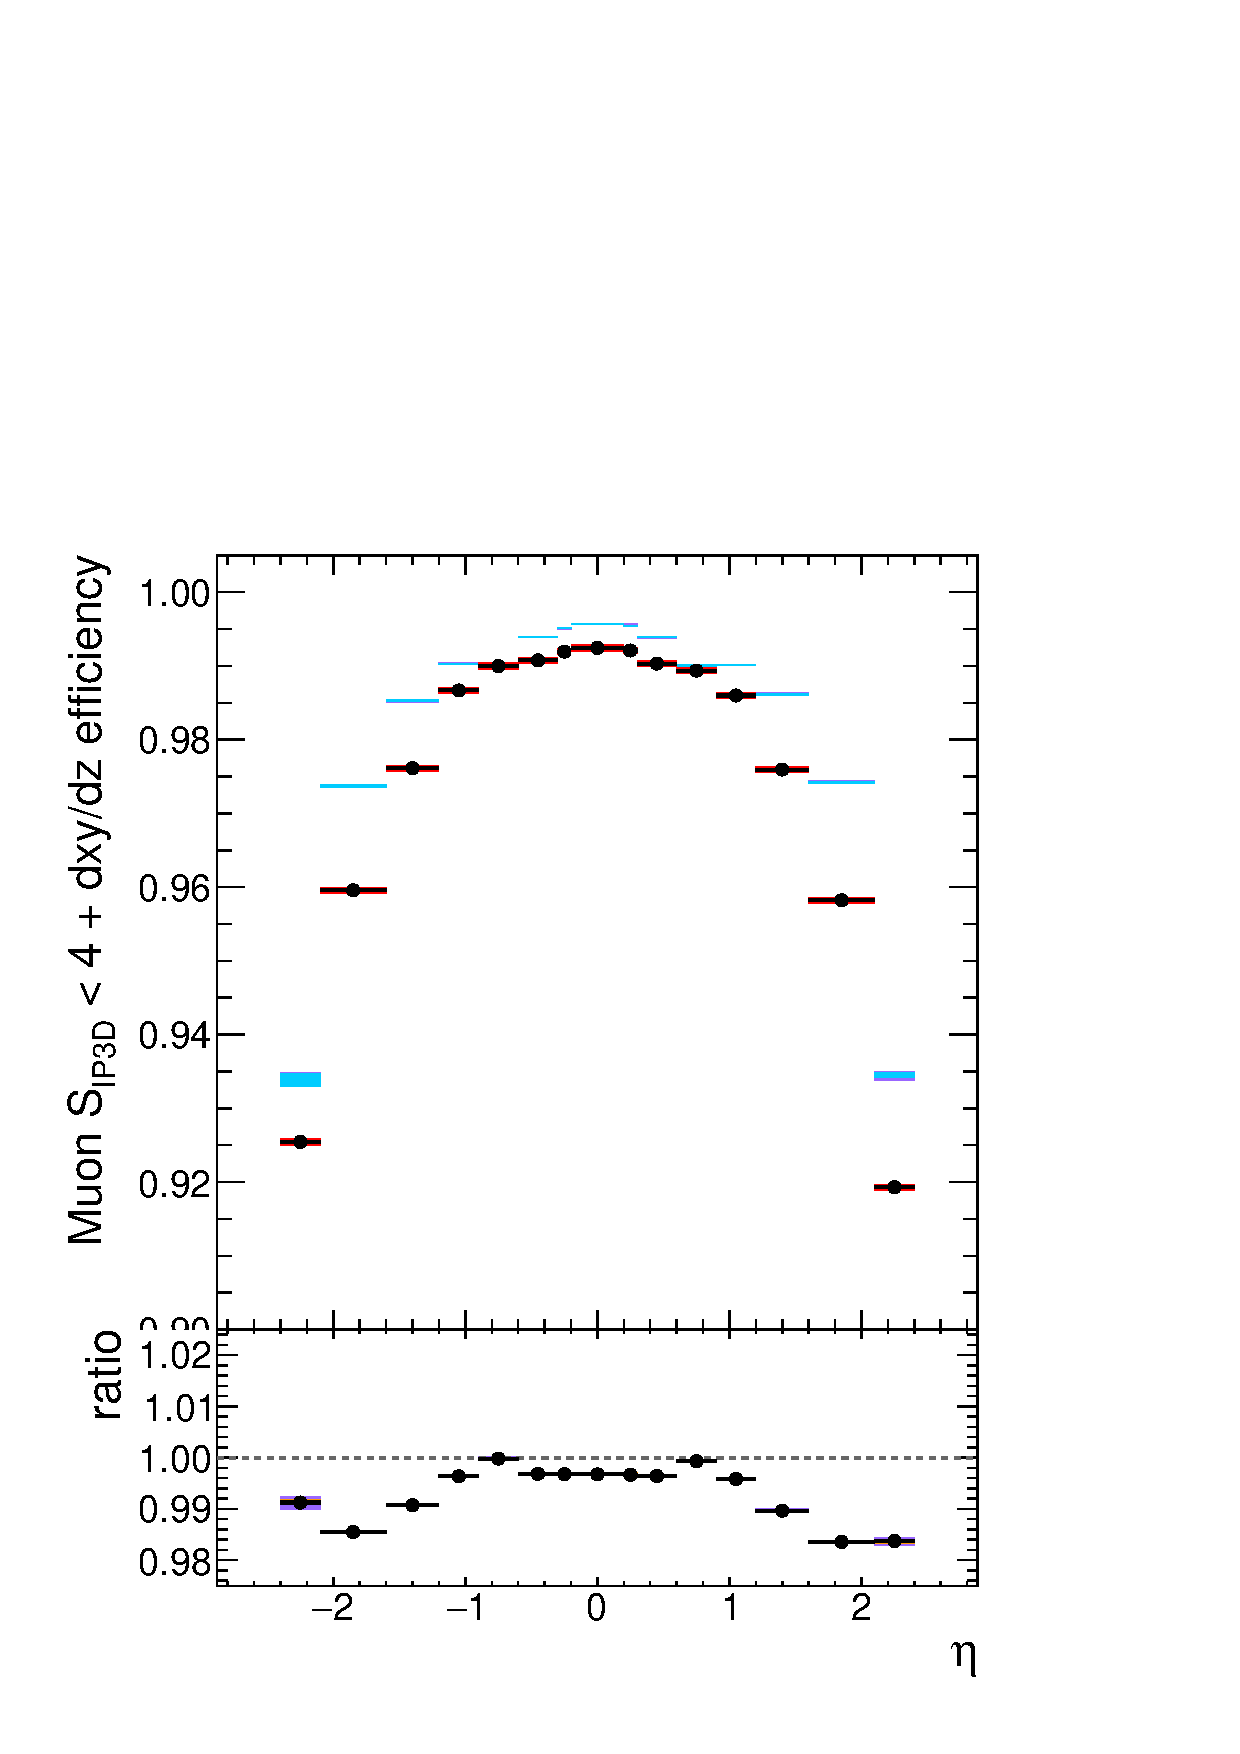
\includegraphics[width=0.32\textwidth]{Figures/Muons/mu_SIP4_pt20_2018.pdf}} 
    \caption{Efficiency of the muon impact parameter requirements, measured with the tag\&probe method on \Z events, as function of \pt in the barrel (left) and endcaps (center), and as function of $\eta$ for $\pt > 20\GeV$ (right), for 2016 (top), 2017 (middle) and 2018 (bottom). In the upper panel, the larger error bars include also the systematical uncertainties, while the smaller ones are purely statistical. In the lower panel showing the ratio of the two efficiencies, the black error bars are for the statistical uncertainty, the orange rectangles for the systematical uncertainty and the violet rectangles include both uncertainties.}
    \label{fig:MuonIDEff_2}
\end{center}
\end{figure}

\paragraph*{Isolation requirements}
The isolation efficiency is measured using events from the $\Z$ decay for any \pt. The events are selected with the triggers as required for impact parameter requirements measurements as explained in previous paragarph. To fit the FSR contribution in the low mass region, MC template convoluted with the Gaussian is used to better fit the dimuon invariant mass. 
%The isolation of the muons are calculated after recovery of the FSR photons and subtracting their contribution to the isolation cone of the muons. More detailed description of the method can be found in Ref.~\cite{AN-16-217}.

The results are shown in Fig.~\ref{fig:MuonIDEff_3}.
\begin{figure}[htbp]
  \begin{center}
    \subfigure[]{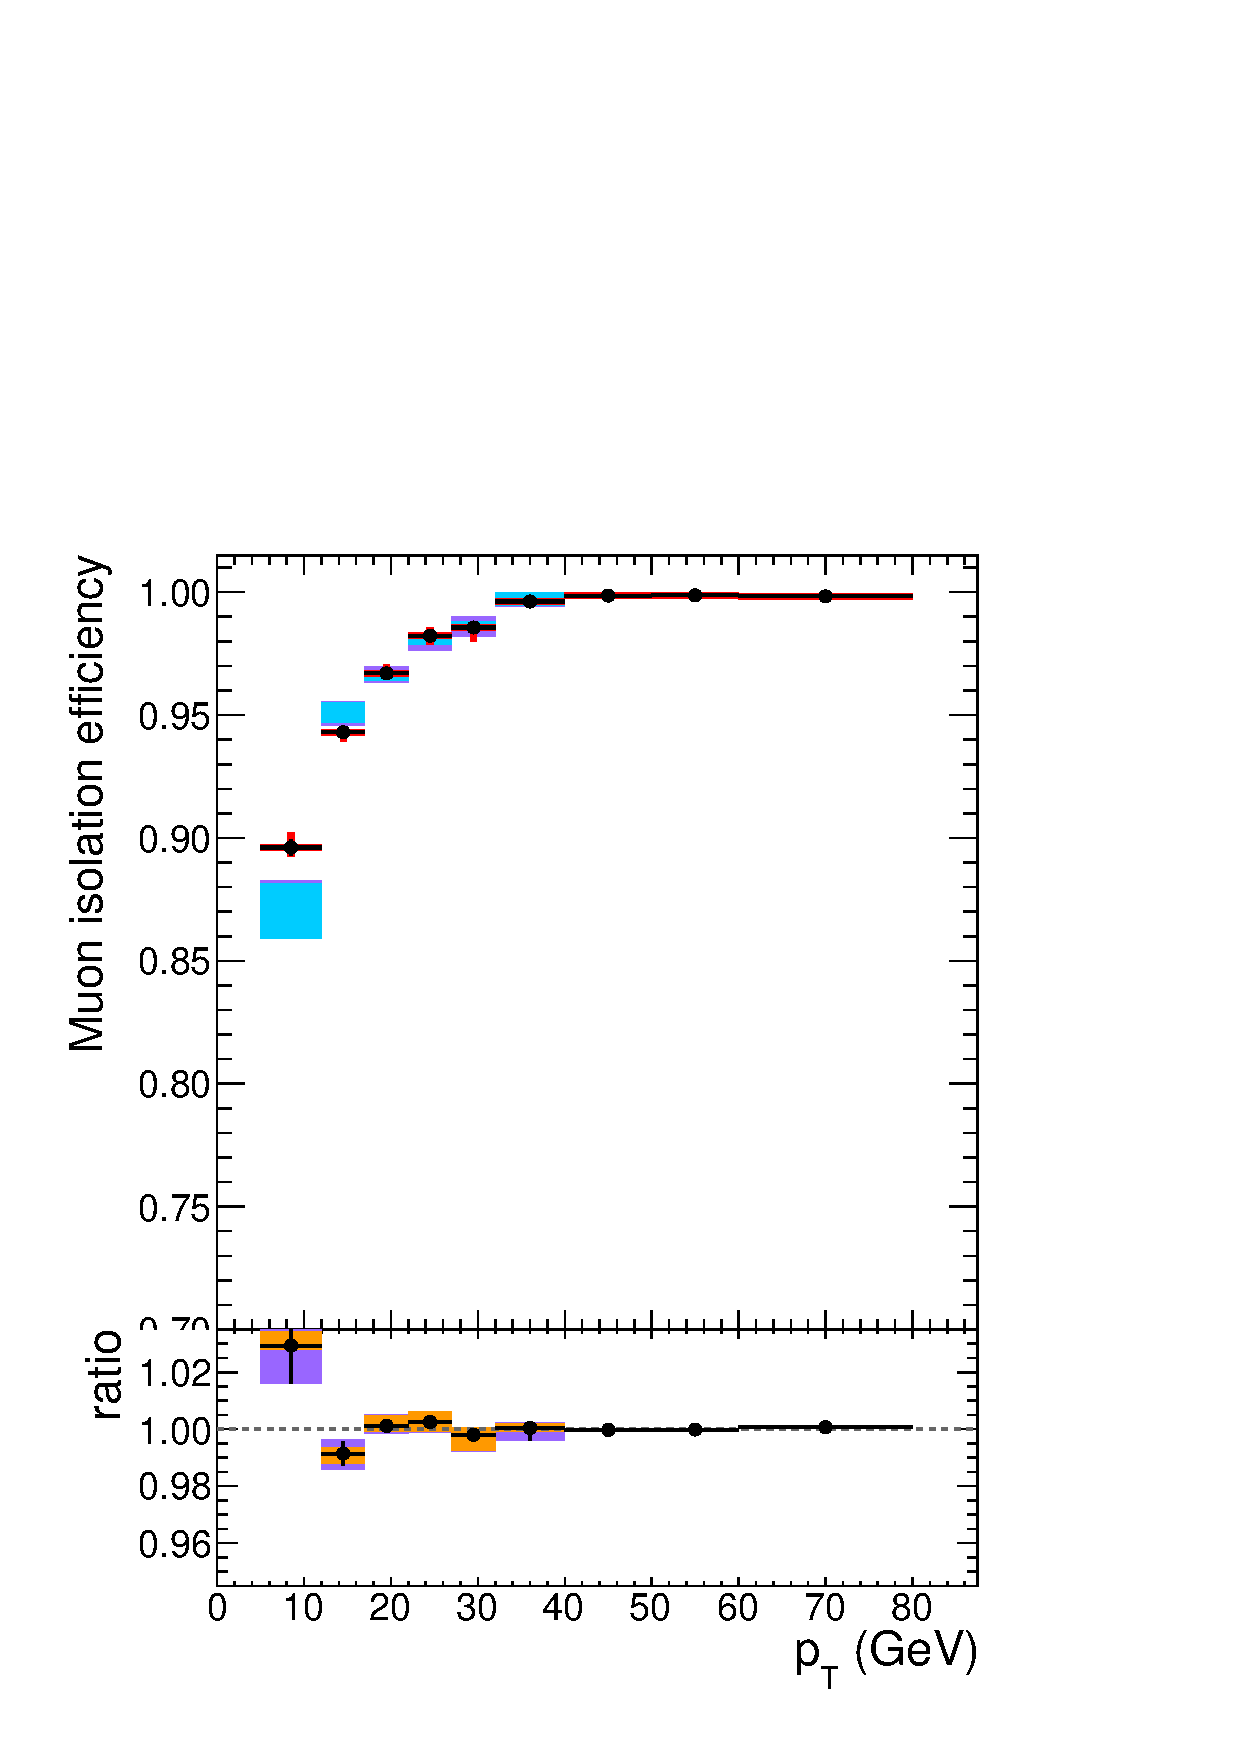
\includegraphics[width=0.32\textwidth]{Figures/Muons/mu_Iso_barrel_2016.pdf}}
    \subfigure[]{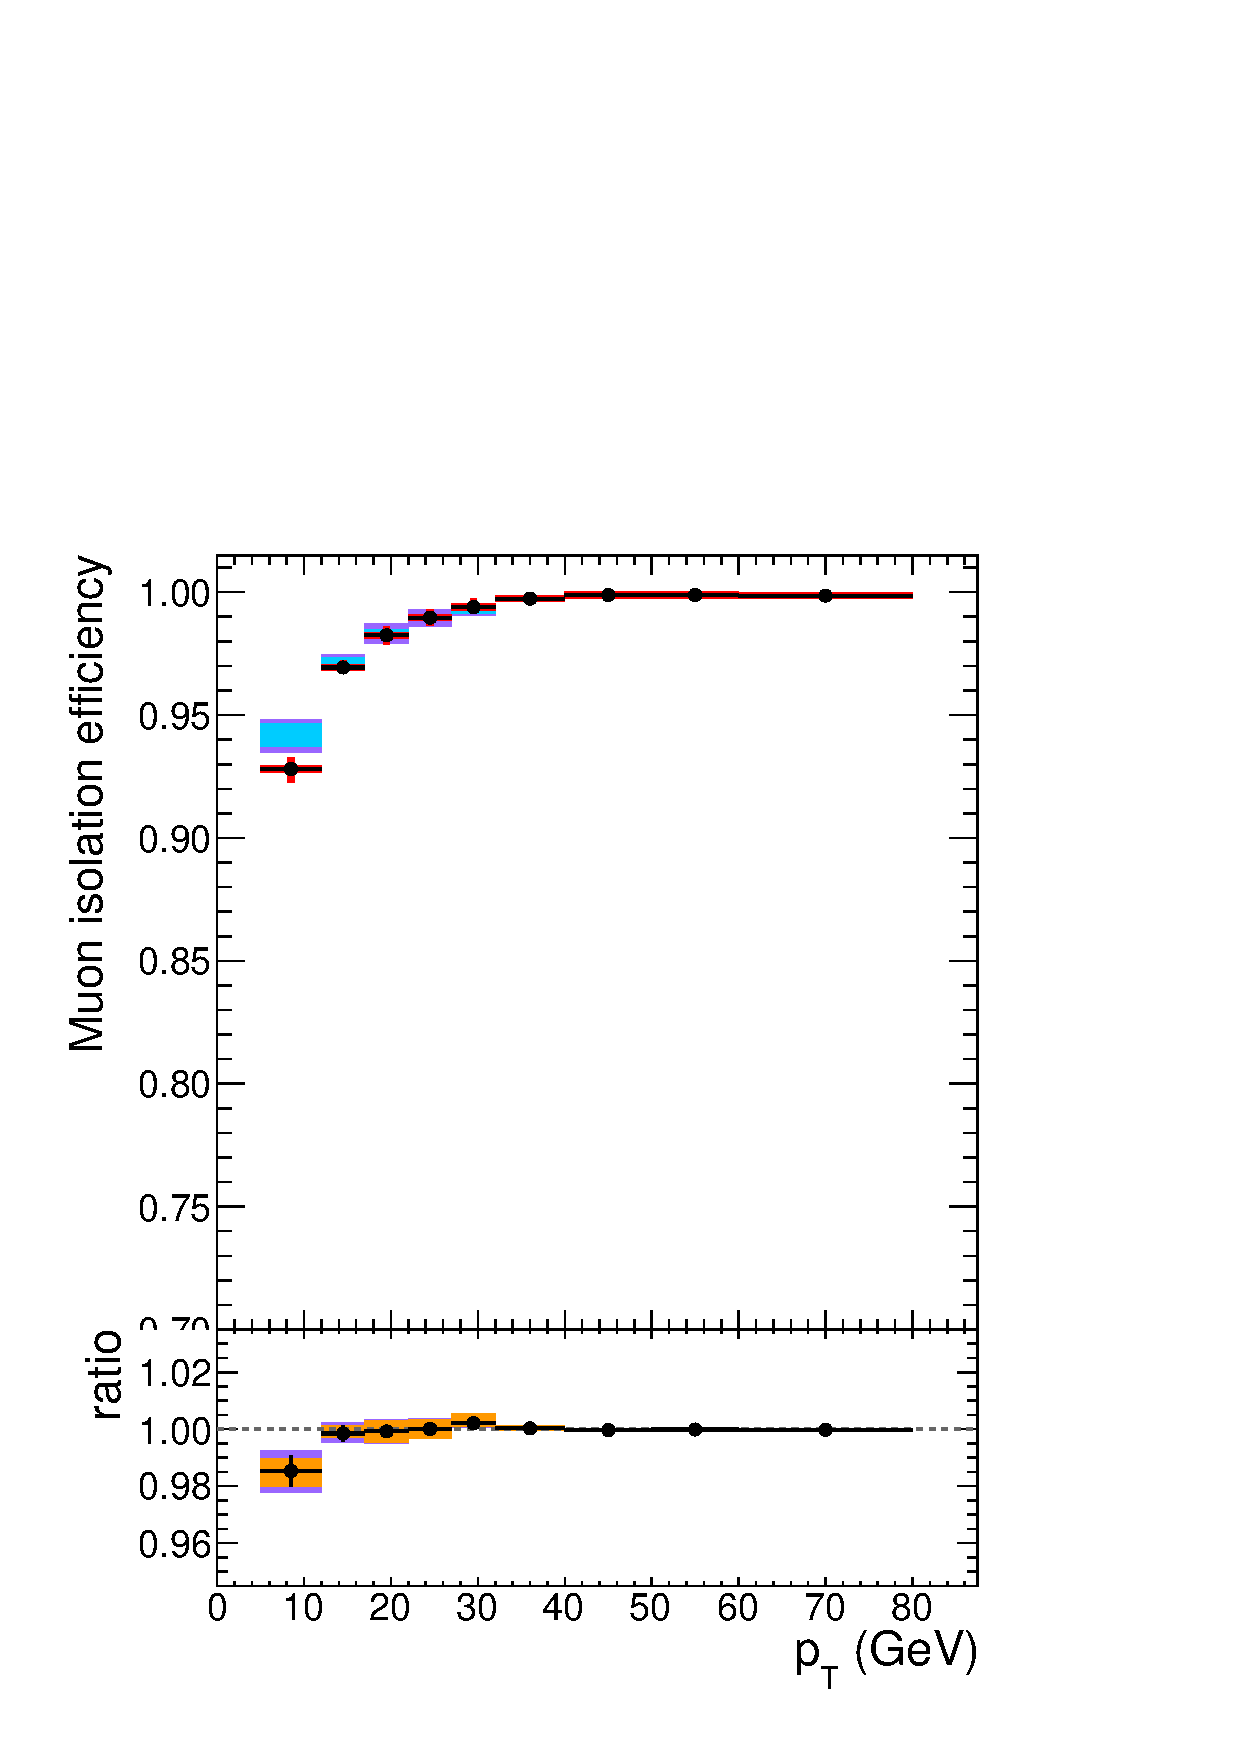
\includegraphics[width=0.32\textwidth]{Figures/Muons/mu_Iso_endcap_2016.pdf}} \\
		\subfigure[]{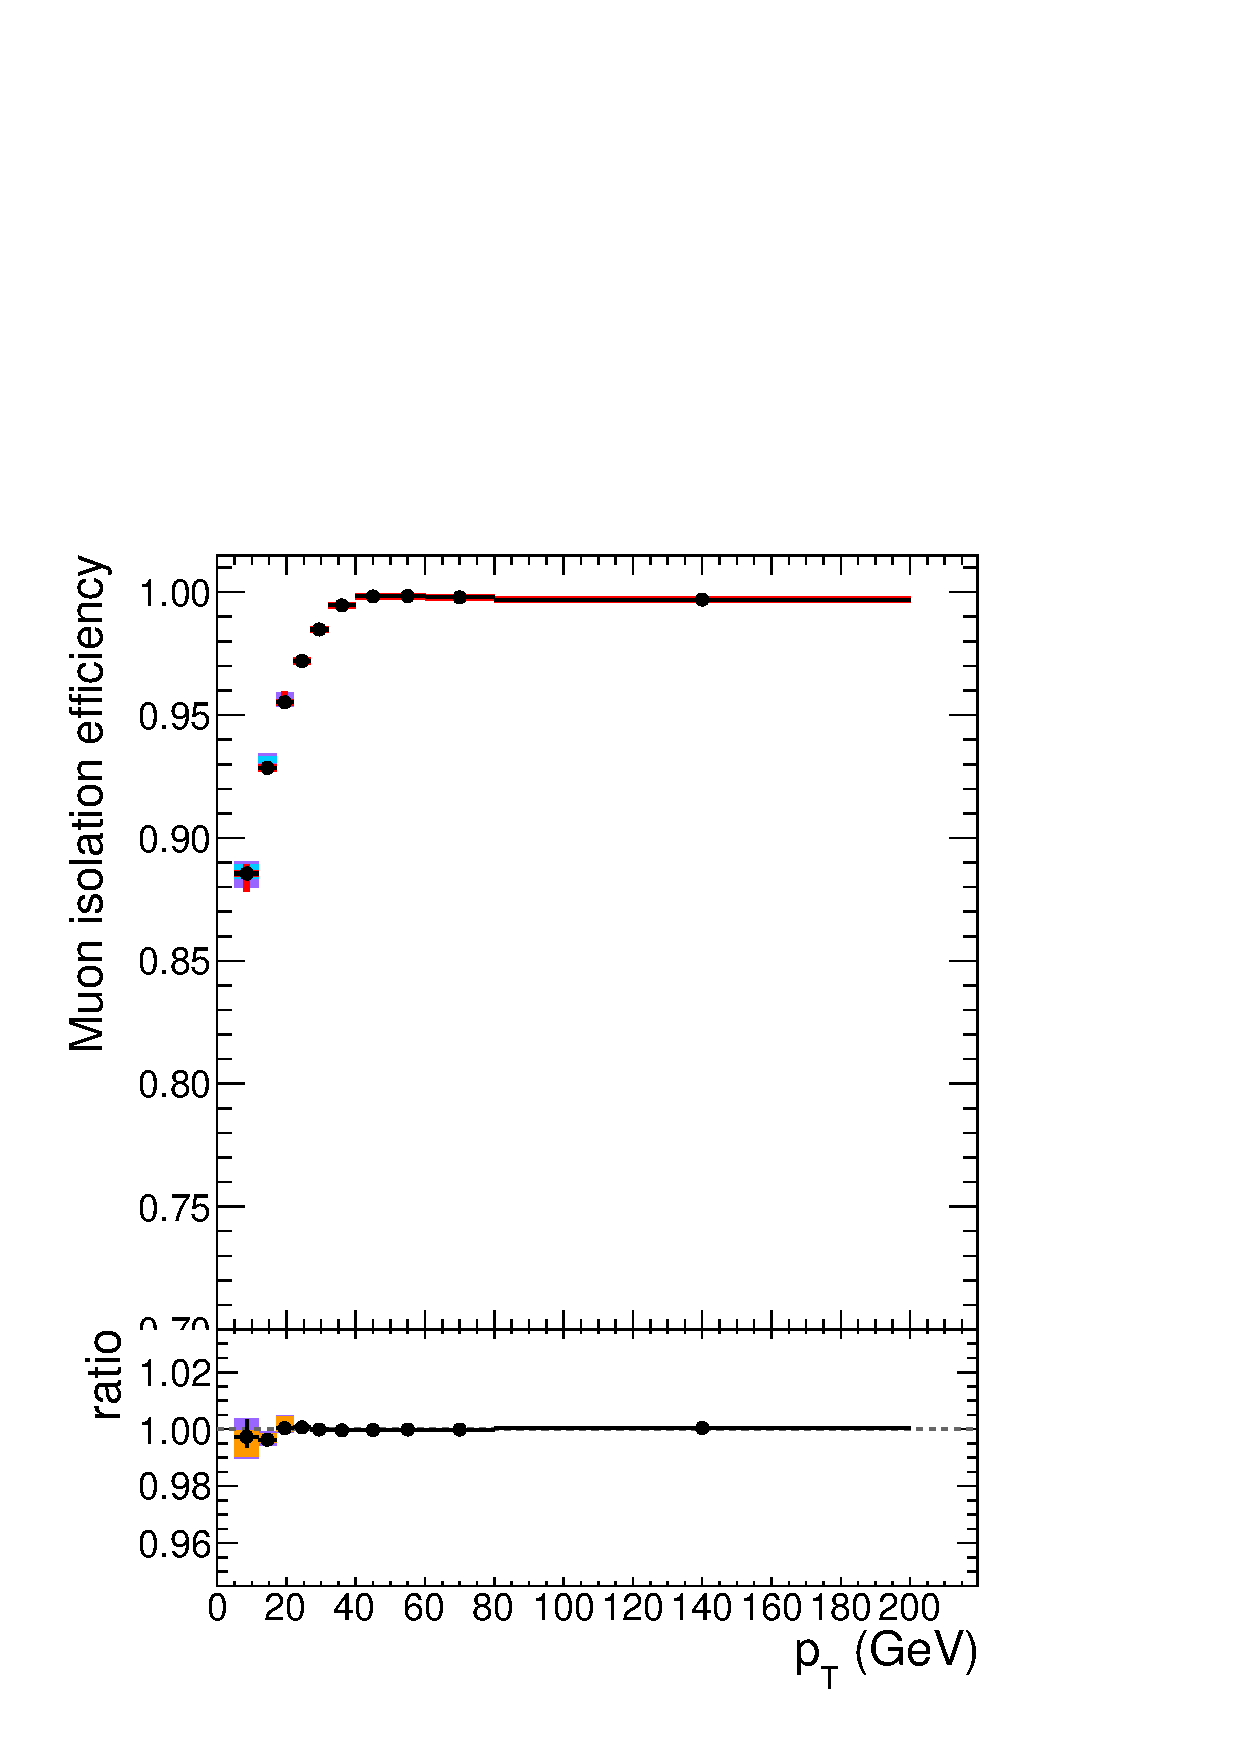
\includegraphics[width=0.32\textwidth]{Figures/Muons/mu_Iso_barrel_2017.pdf}}
    \subfigure[]{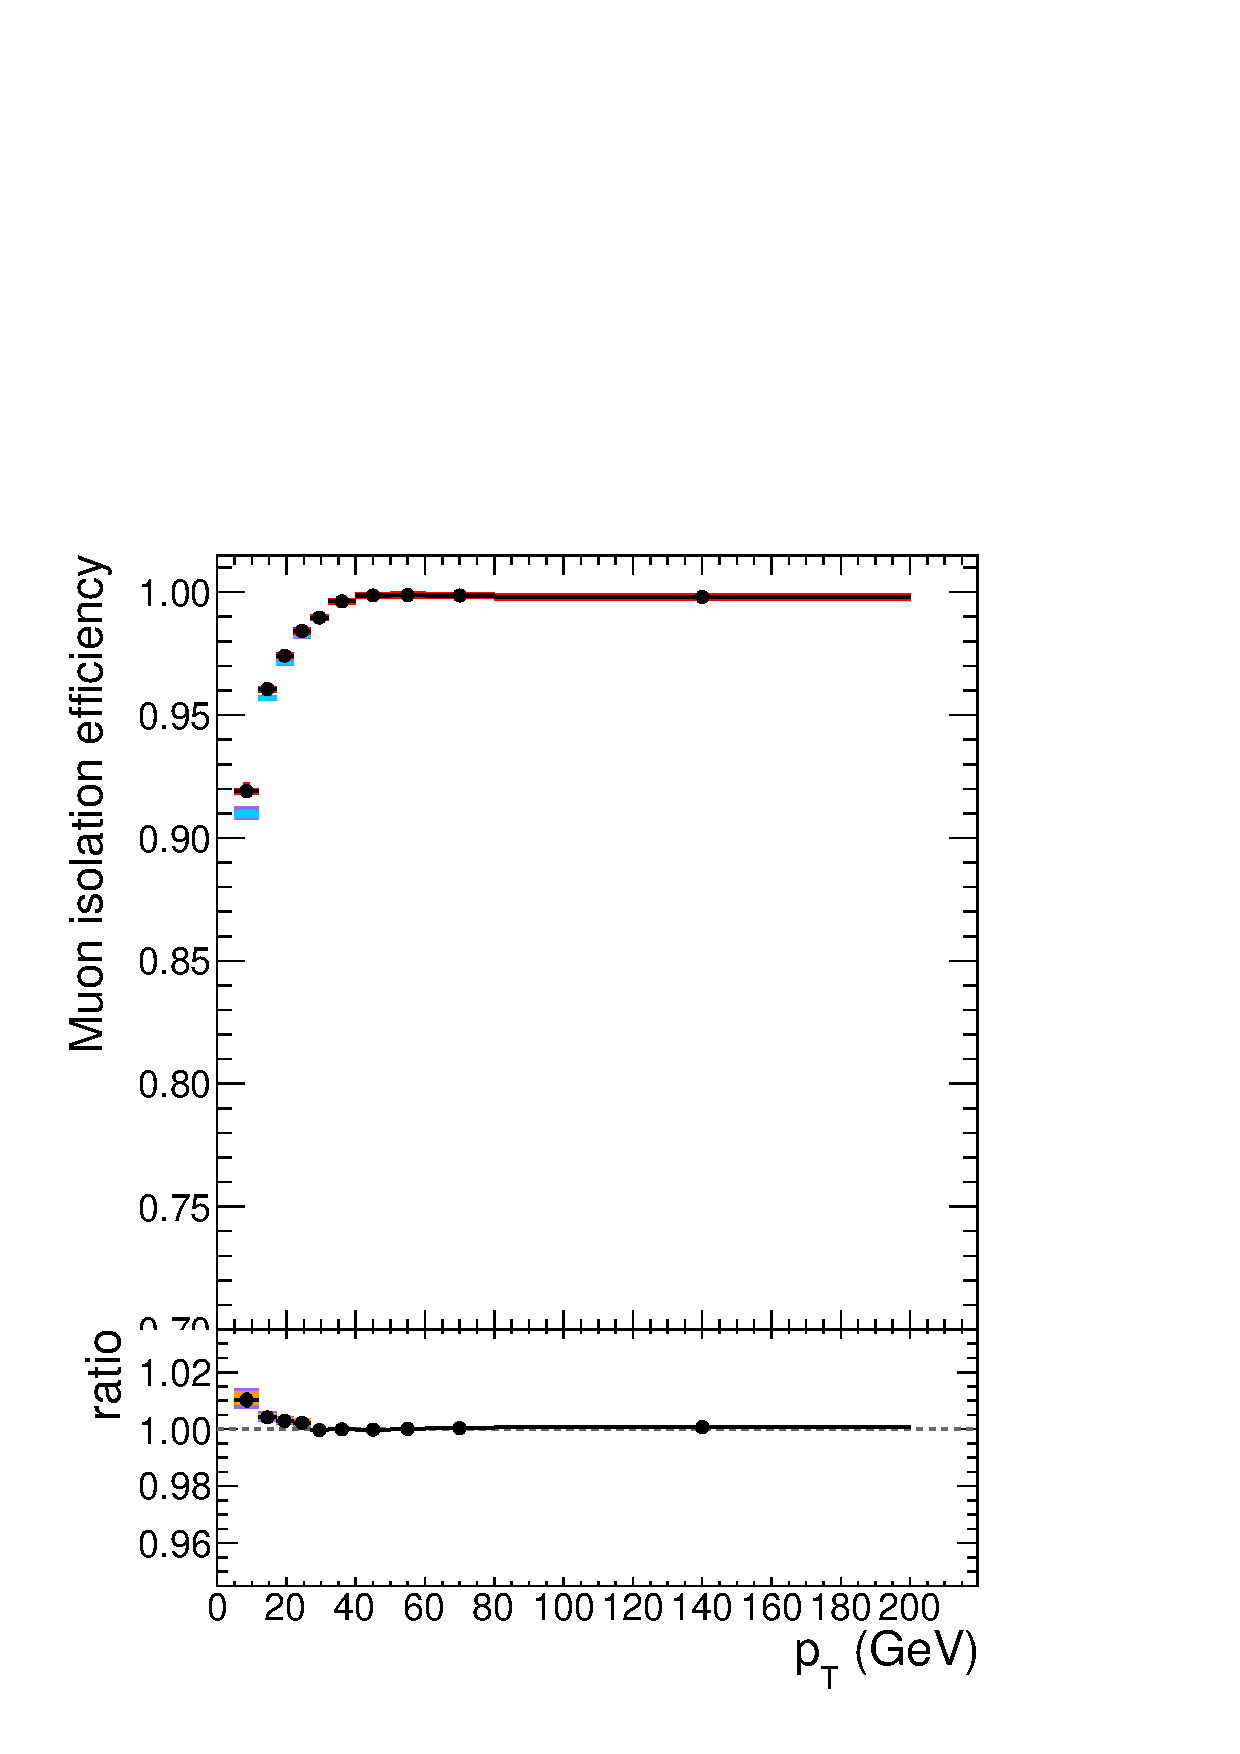
\includegraphics[width=0.32\textwidth]{Figures/Muons/mu_Iso_endcap_2017.pdf}} \\ 
		\subfigure[]{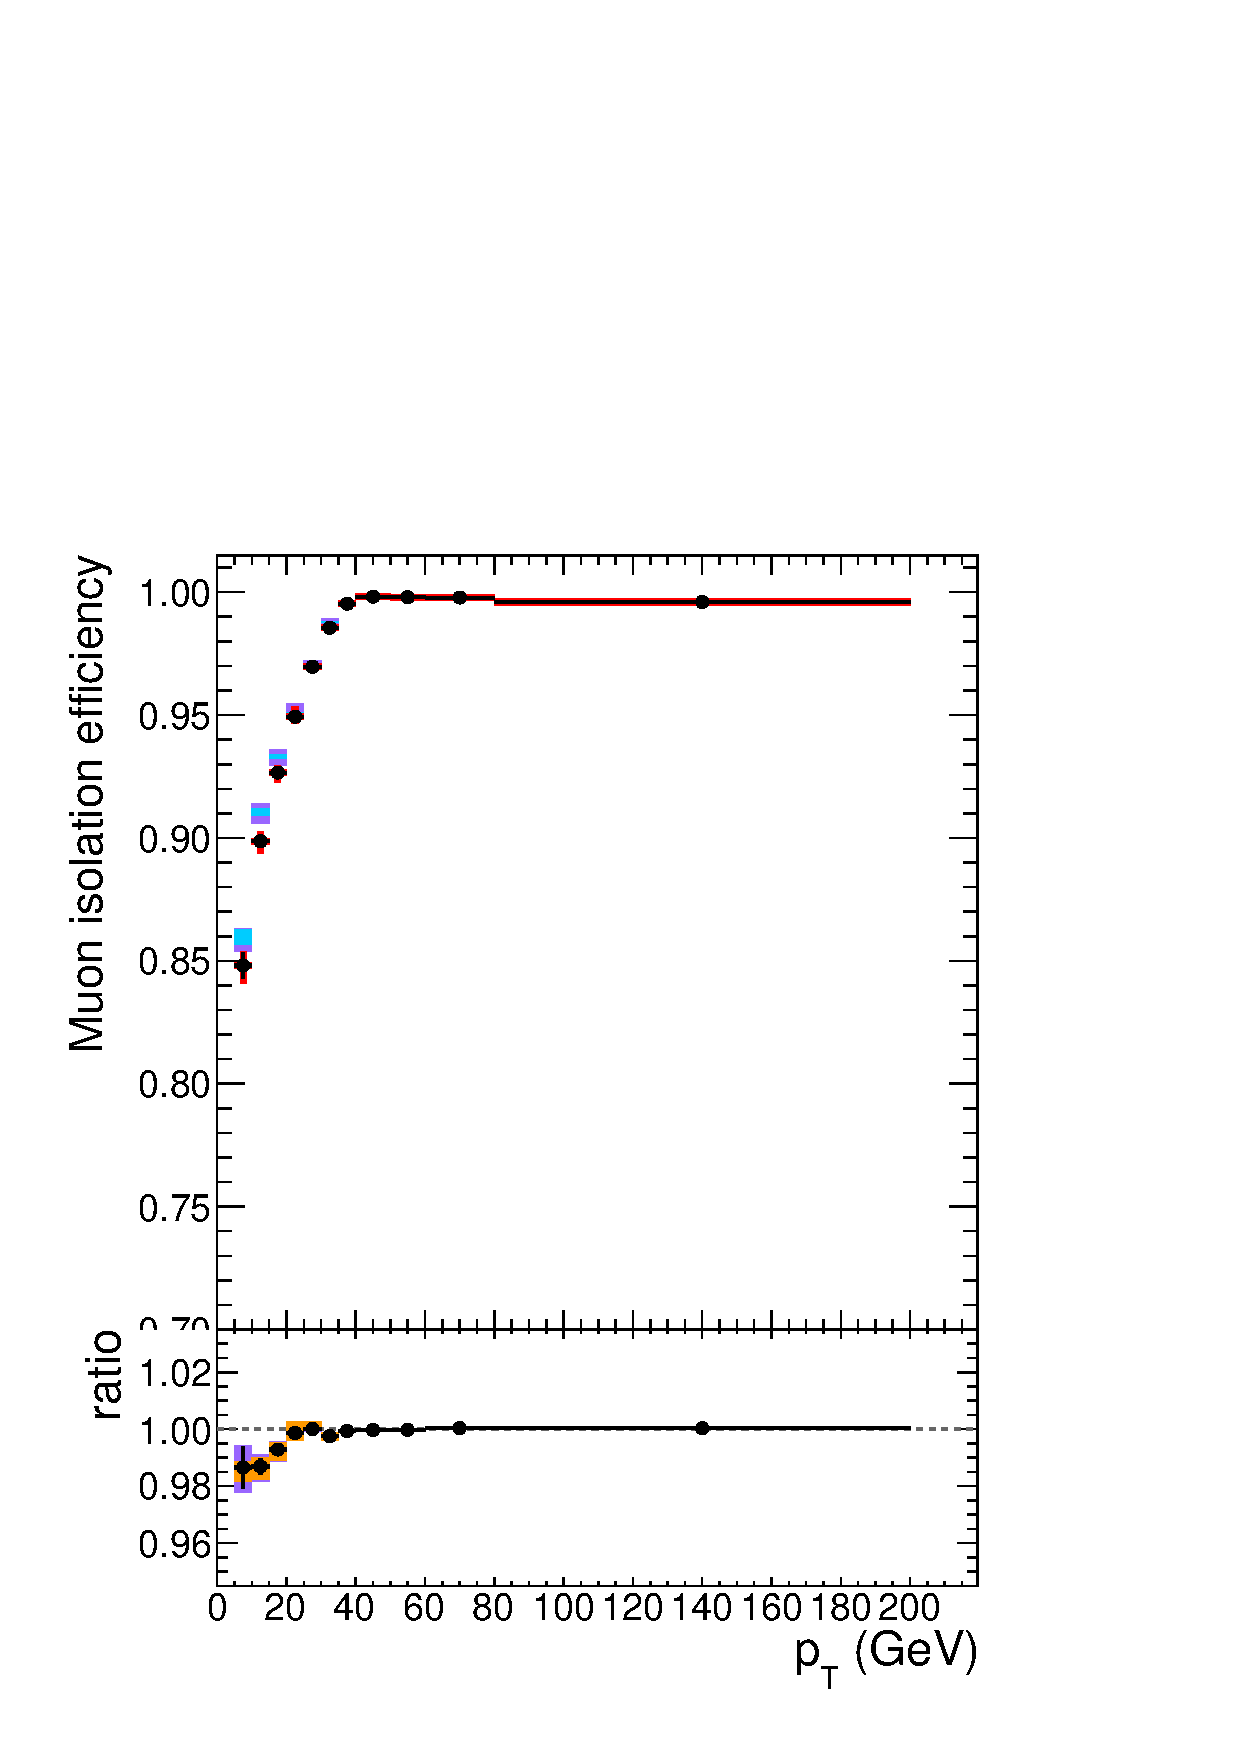
\includegraphics[width=0.32\textwidth]{Figures/Muons/mu_Iso_barrel_2018.pdf}}
    \subfigure[]{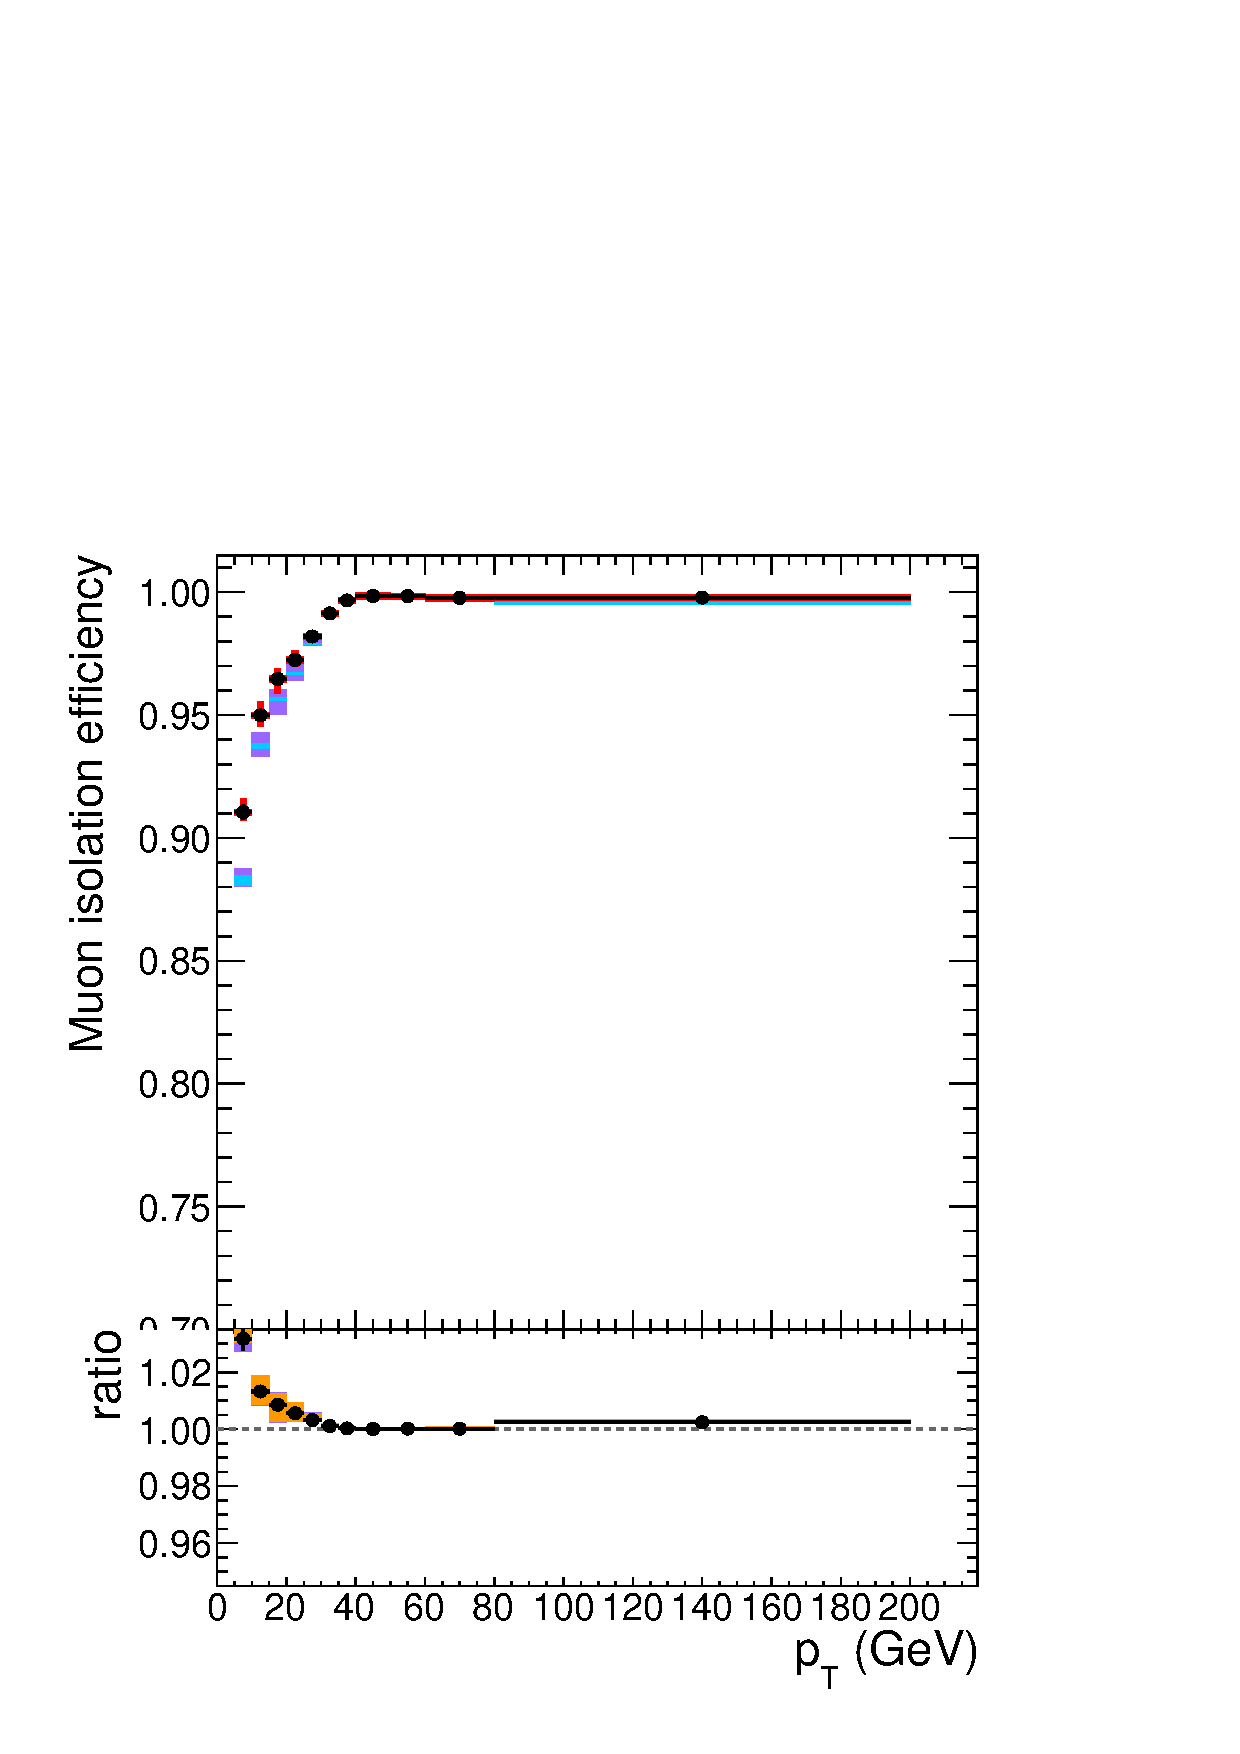
\includegraphics[width=0.32\textwidth]{Figures/Muons/mu_Iso_endcap_2018.pdf}} 
    \caption{Efficiency of the muon isolation requirement, measured with the tag\&probe method on \Z events, as function of \pt in the barrel (left) and endcaps (right), for 2016 (top), 2017 (middle) and 2018 (bottom). In the upper panel, the larger error bars include also the systematical uncertainties, while the smaller ones are purely statistical. In the lower panel showing the ratio of the two efficiencies, the black error bars are for the statistical uncertainty, the orange rectangles for the systematical uncertainty and the violet rectangles include both uncertainties.}
    \label{fig:MuonIDEff_3}
\end{center}
\end{figure}

\paragraph*{Tracking}
The efficiency to reconstruct a muon track in the inner detector can be measured using as probes tracks
reconstructed in the muon system alone. However, since it comes out to be 100\%, it is no more recommended by muon POG. 
%The method for measuring the tracking efficiency is the same as 
% in Ref.~\cite{CMS_AN_2015-215}, and the results on 2018 data are briefly discussed here. The efficiency and 
%data to mc scale factors are measured from Z events as a function of $\eta$ for $\pt > 10\GeV$ and $\pt < 10\GeV$. The values of data to mc scale factors 
%used are from the ReReco version of the full dataset collected in 2018. 

%The tracking efficiency in data and simulation as a function of $\eta$ is shown in Fig.~\ref{fig:MuonIDEff_4}.
%\begin{figure}[htbp]
%  \begin{center}
%    \subfigure[]{
\includegraphics[width=0.42\textwidth]{Figures/Muons/Placeholder.png}}
%    \subfigure[]{
\includegraphics[width=0.42\textwidth]{Figures/Muons/Placeholder.png}}
%    \caption{Tracking efficiency in data and simulation as a function of $\eta$ for muon $\pt < 10\GeV$(left) and $\pt > 10\GeV$(right) with ReReco data.}
%    \label{fig:MuonIDEff_4}
%\end{center}
%\end{figure}

\paragraph*{Overall results}
The product of all the data to simulation scale factors for muon tracking, reconstruction, identification, impact parameter and isolation requirements is shown in Fig.~\ref{fig:MuonIDEff_5}. 
The systematic effects on measurements are estimated by \footnote{For low \pt measurements of reconstruction and identification only first three systematic sources are used as recommended by muon POG}:
%\begin{itemize}
\begin{enumerate}
        \item Varying the analytical signal and background shape models used to fit the dimuon invariant mass
        \item Increasing and decreasing the number of bins in dimuon mass distribution 
        \item Increasing and decreasing the dimuon mass range 
        \item Relaxing and tightening a selection cut on tag muons 
%\end{itemize}
\end{enumerate}

%The overall correction is about $-1\%$ or less for most \pt and $\eta$ values, increasing to about $-2\%$ in for muons below $10\GeV$ or with $|\eta|>2$.
\begin{figure}[htbp]
  \begin{center}
    %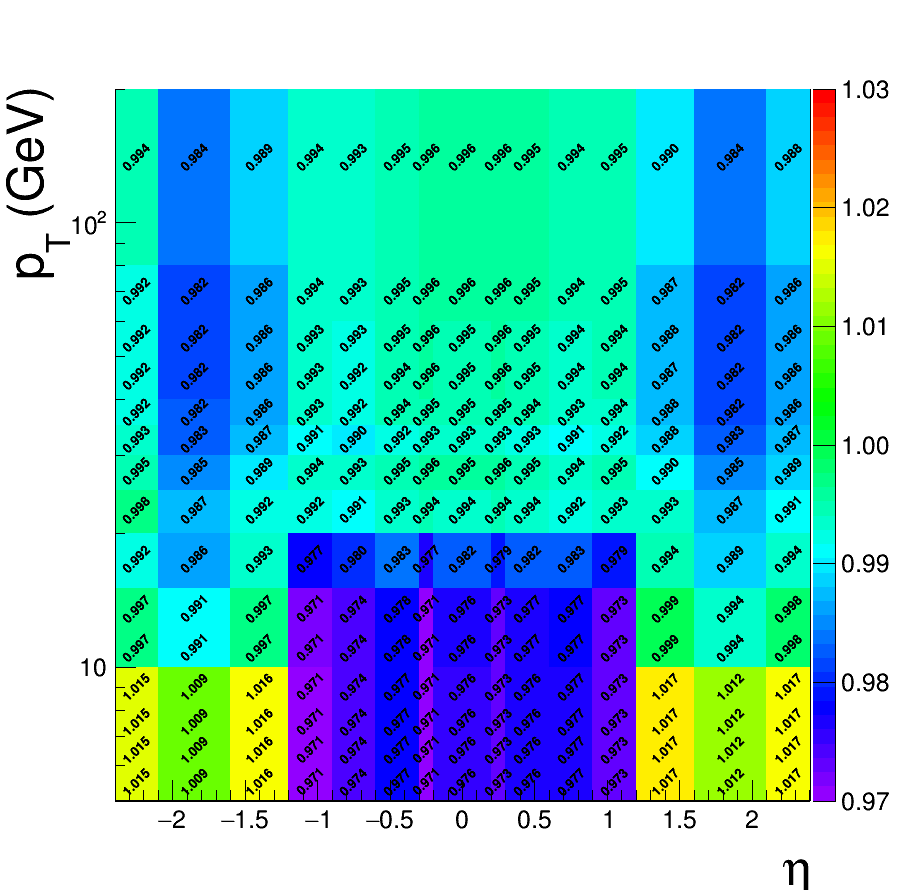
\includegraphics[width=0.45\textwidth]{Figures/Muons/HZZ_SF_2018_RunA2D_2801.png}
    %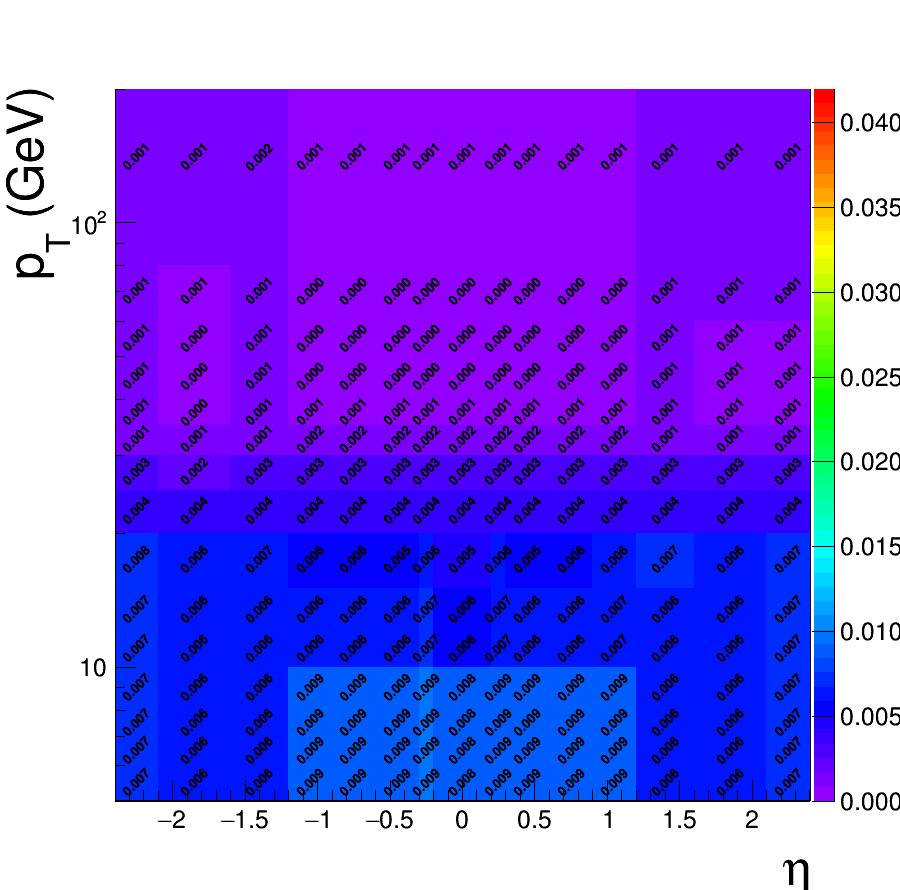
\includegraphics[width=0.45\textwidth]{Figures/Muons/HZZ_SF_errors_2018_RunA2D_2801.png}
		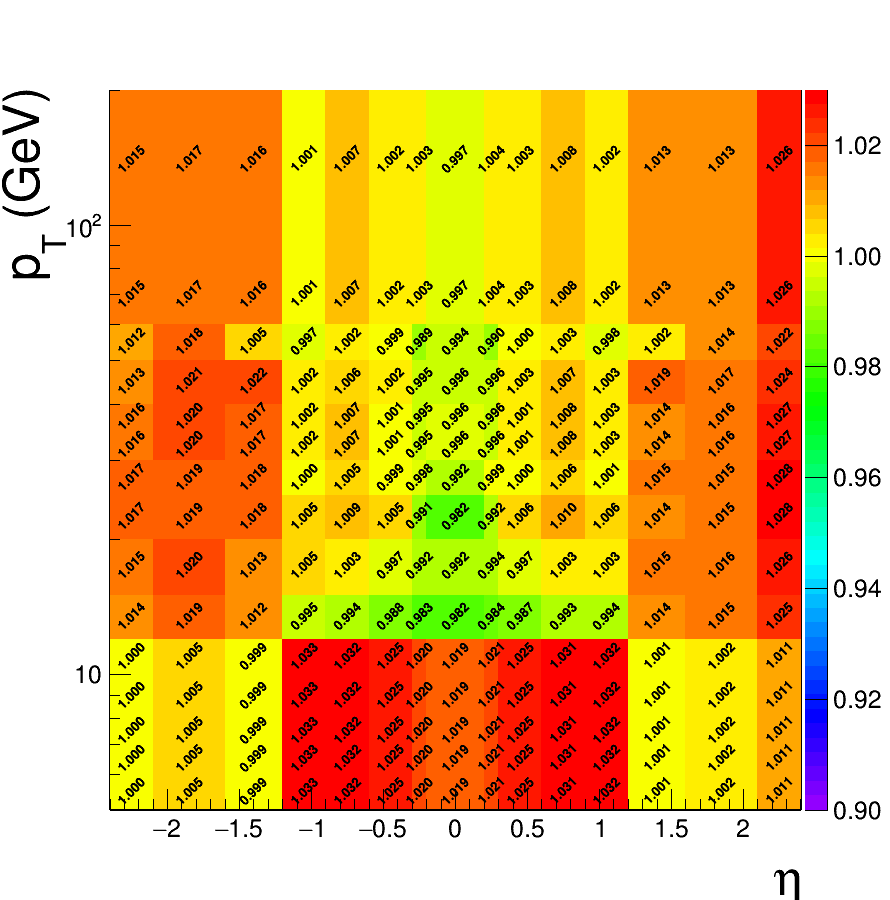
\includegraphics[width=0.45\textwidth]{Figures/Muons/2016_SF_legacy_newLoose.png}
    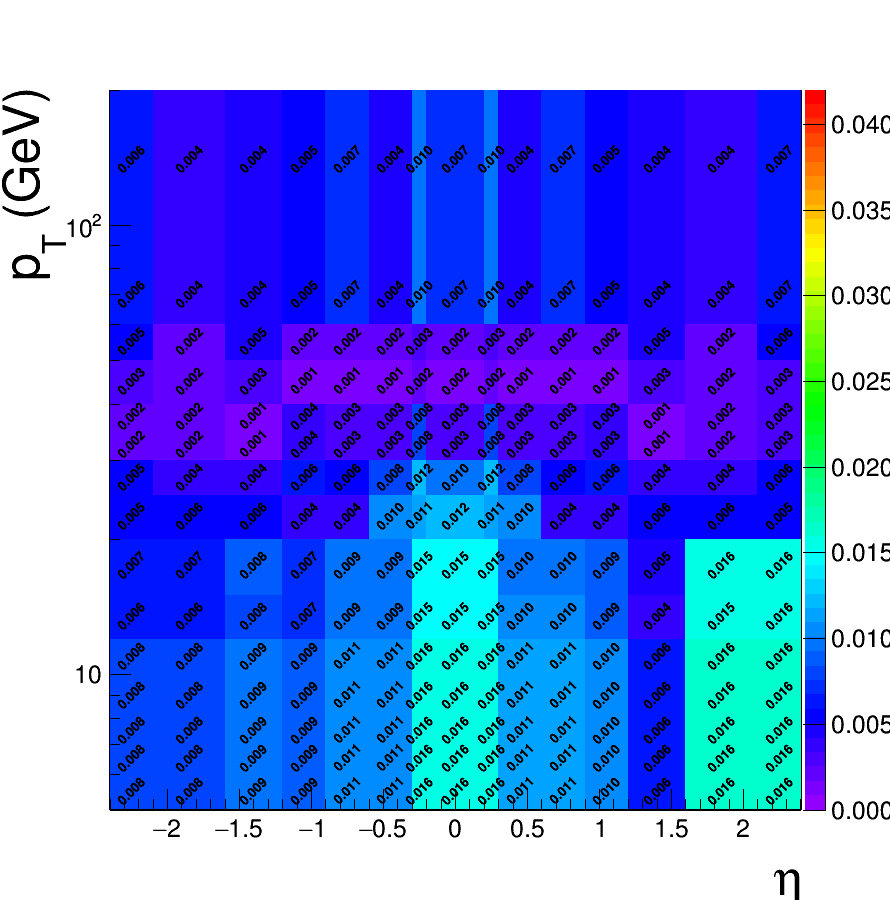
\includegraphics[width=0.45\textwidth]{Figures/Muons/2016_SF_errors_legacy_newLoose.png} \\
		%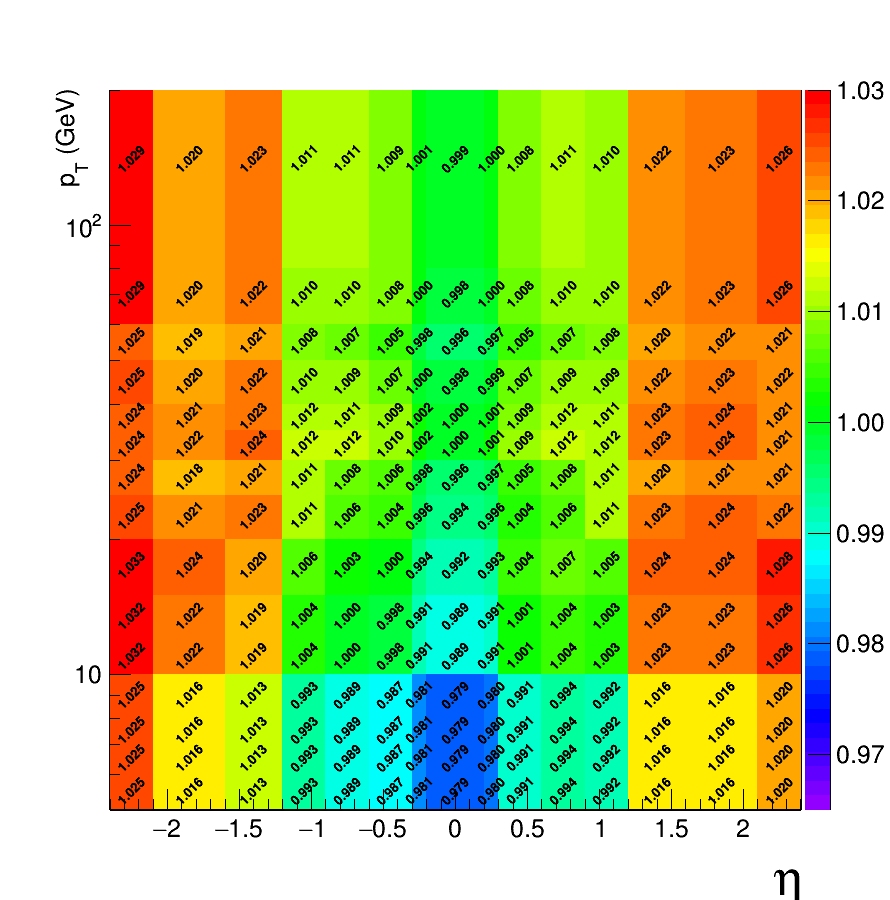
\includegraphics[width=0.45\textwidth]{Figures/Muons/2017_SF_rereco_LooseGT20syst.png}
		%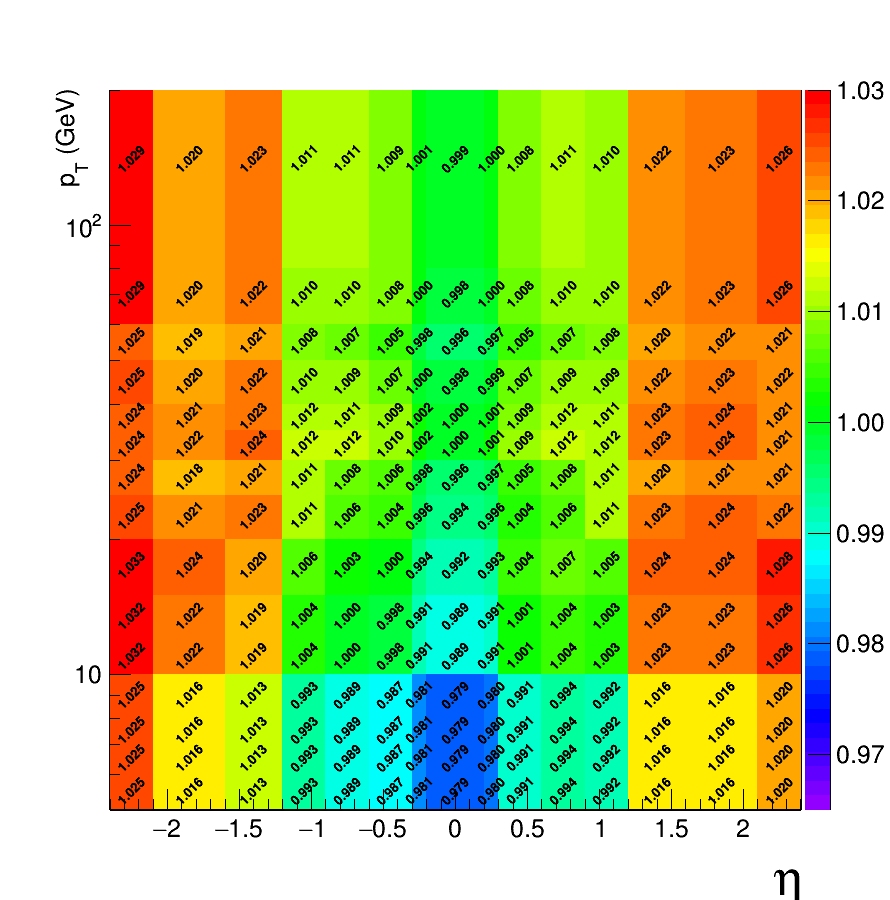
\includegraphics[width=0.45\textwidth]{Figures/Muons/2017_SF_rereco_LooseGT20syst.png}
		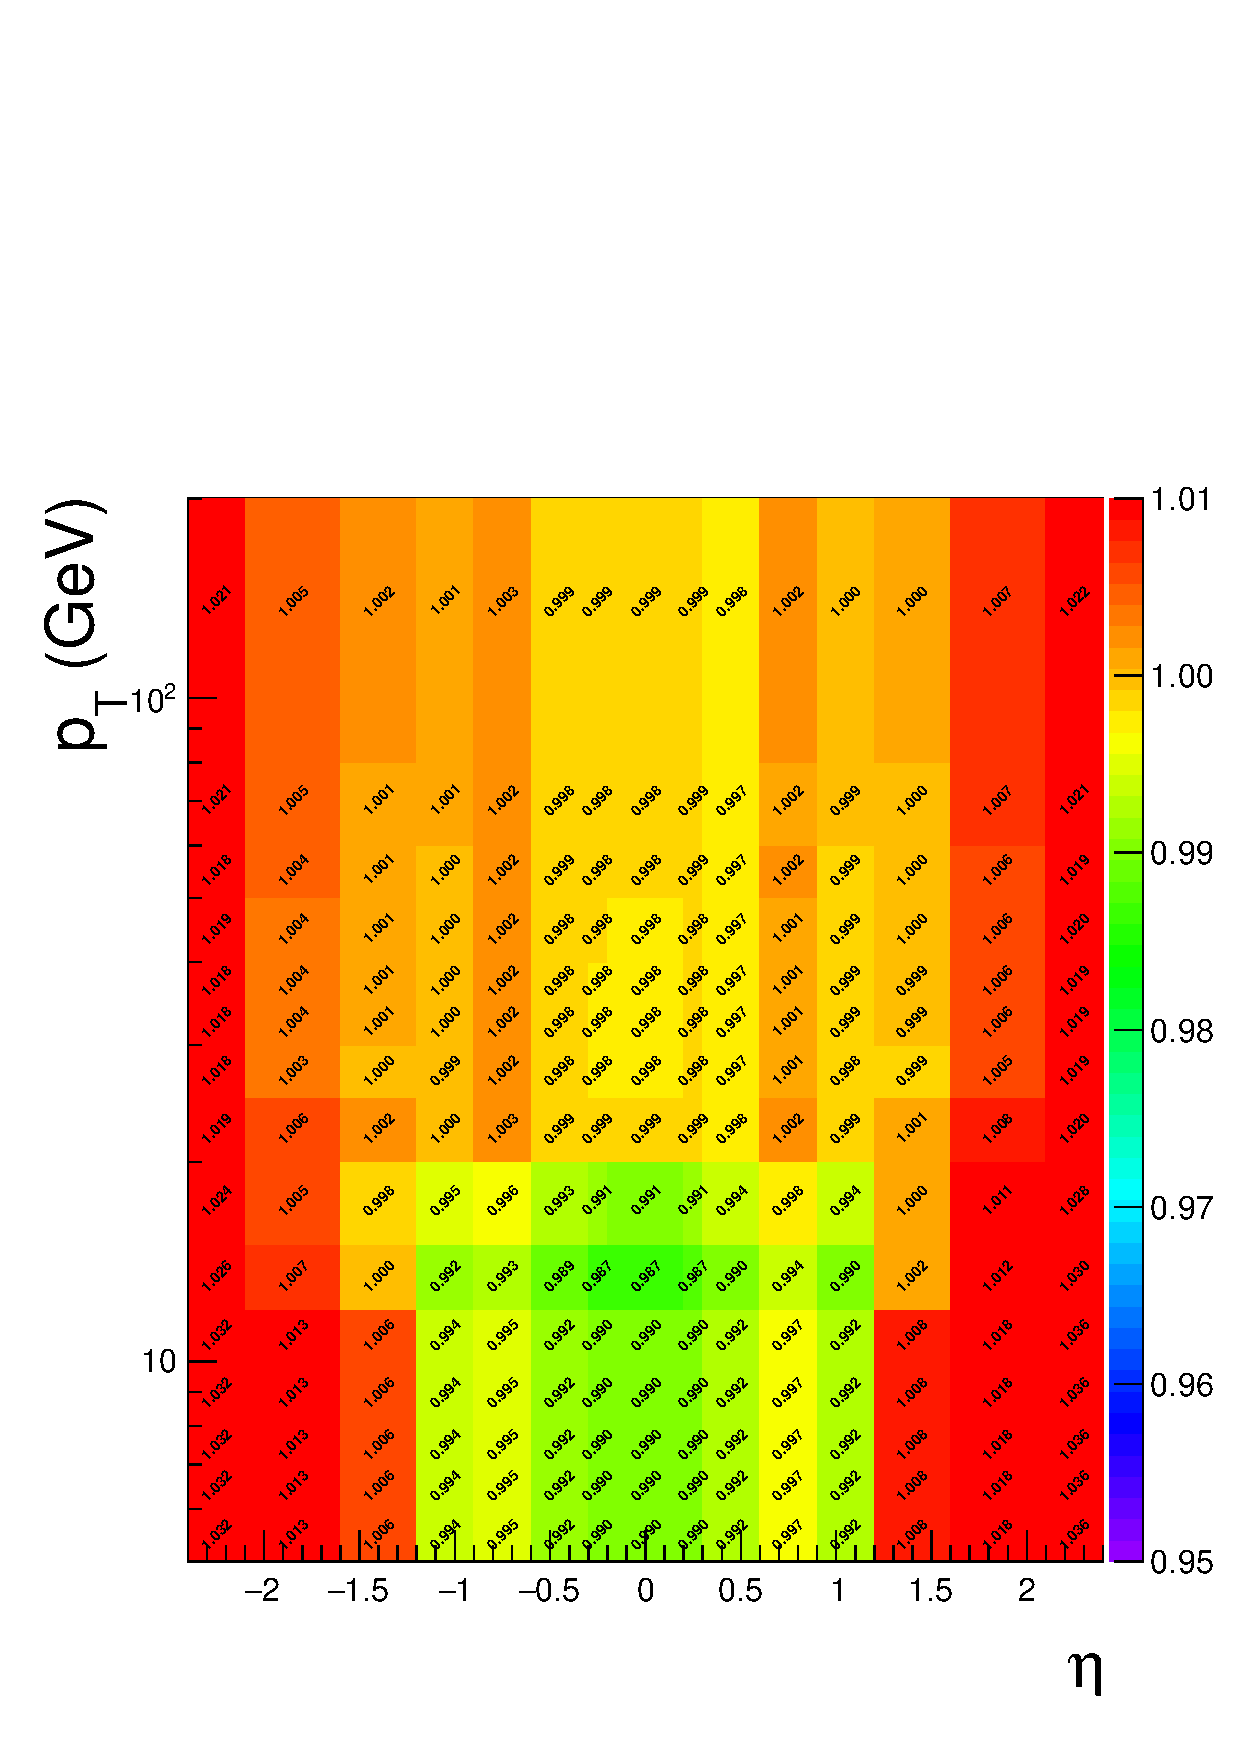
\includegraphics[width=0.45\textwidth]{Figures/Muons/2017UL_SFs.pdf}
    %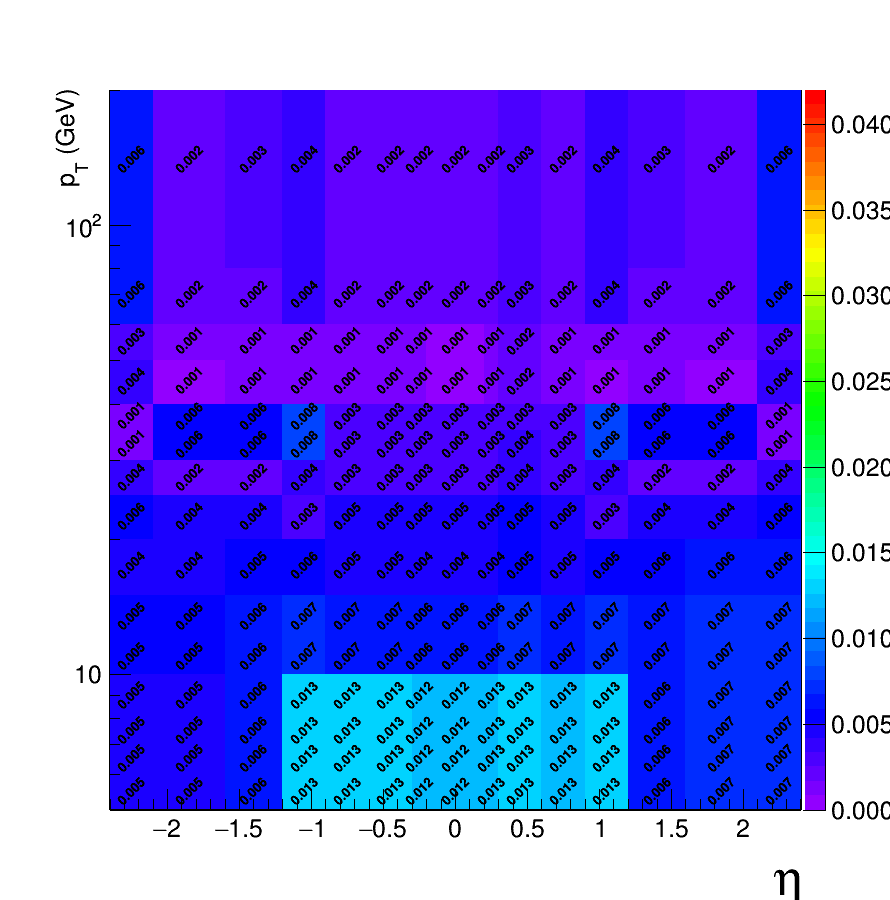
\includegraphics[width=0.45\textwidth]{Figures/Muons/2017_SF_errors_rereco_LooseGT20syst.png} \\
    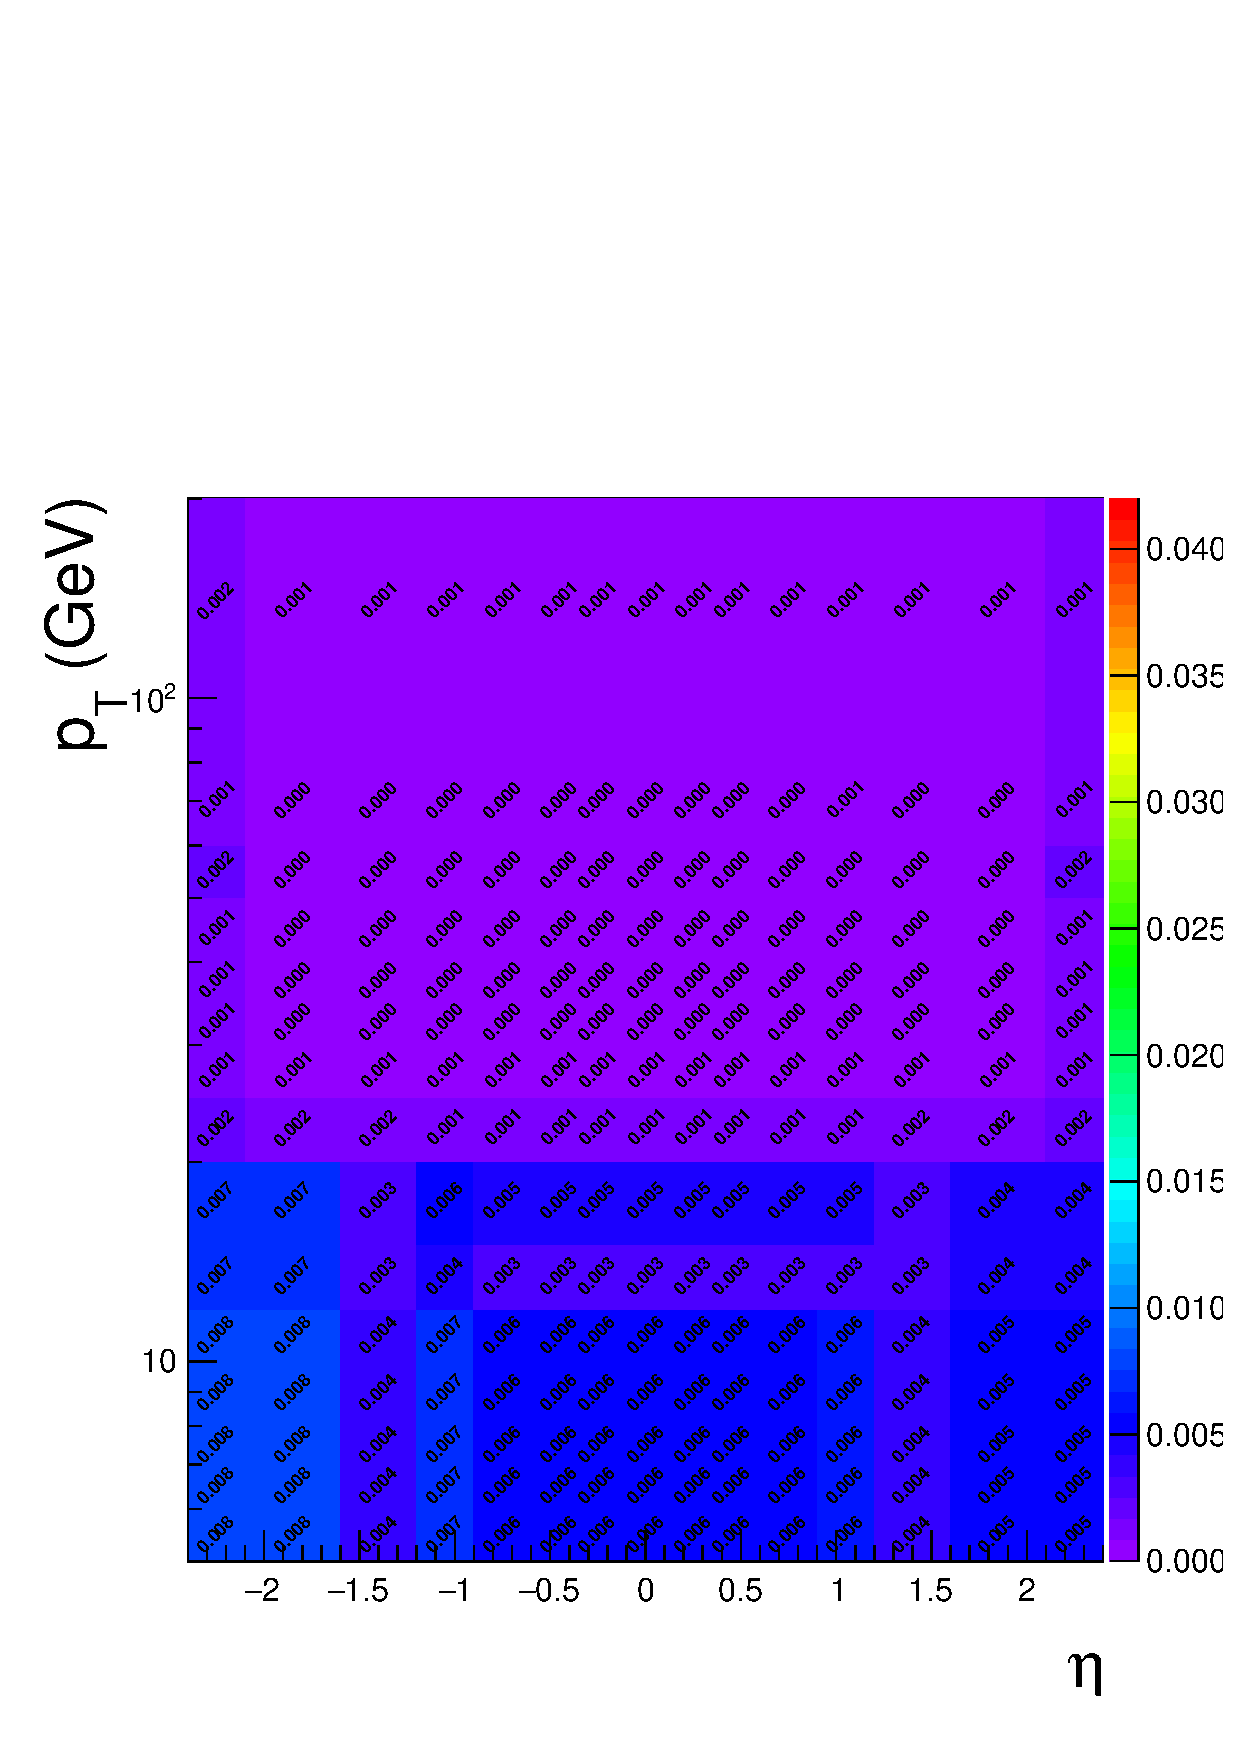
\includegraphics[width=0.45\textwidth]{Figures/Muons/2017UL_SF_errors.pdf} \\
		%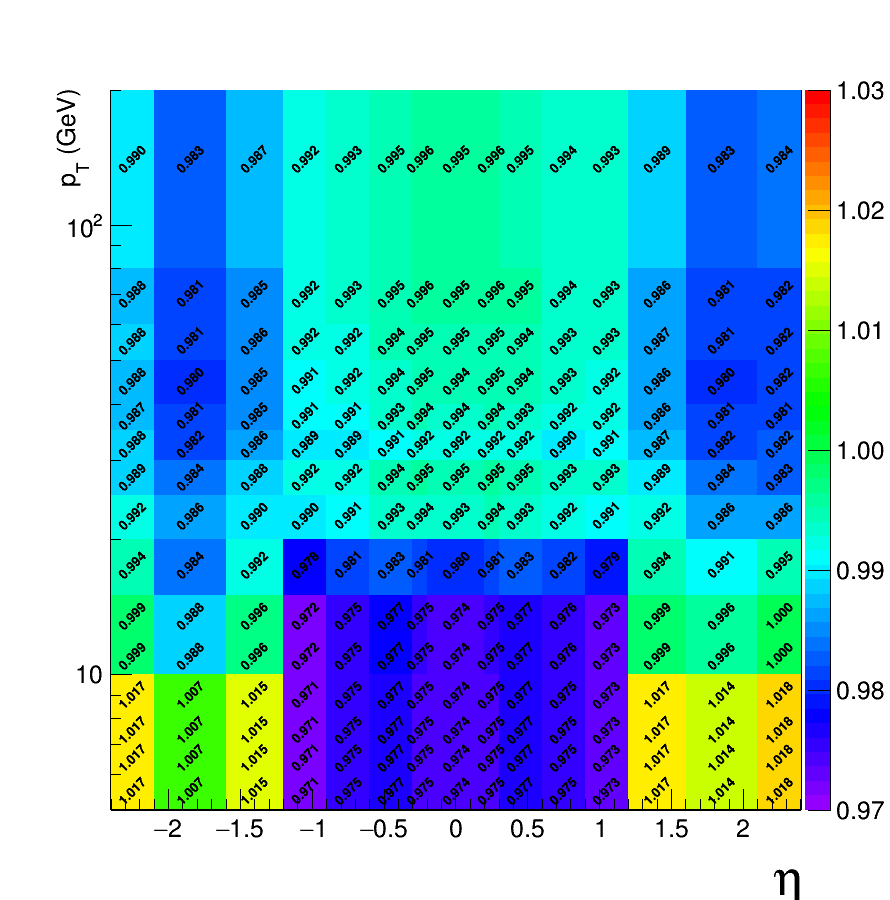
\includegraphics[width=0.45\textwidth]{Figures/Muons/2018_SF_rereco_LooseGT20syst.png} 
		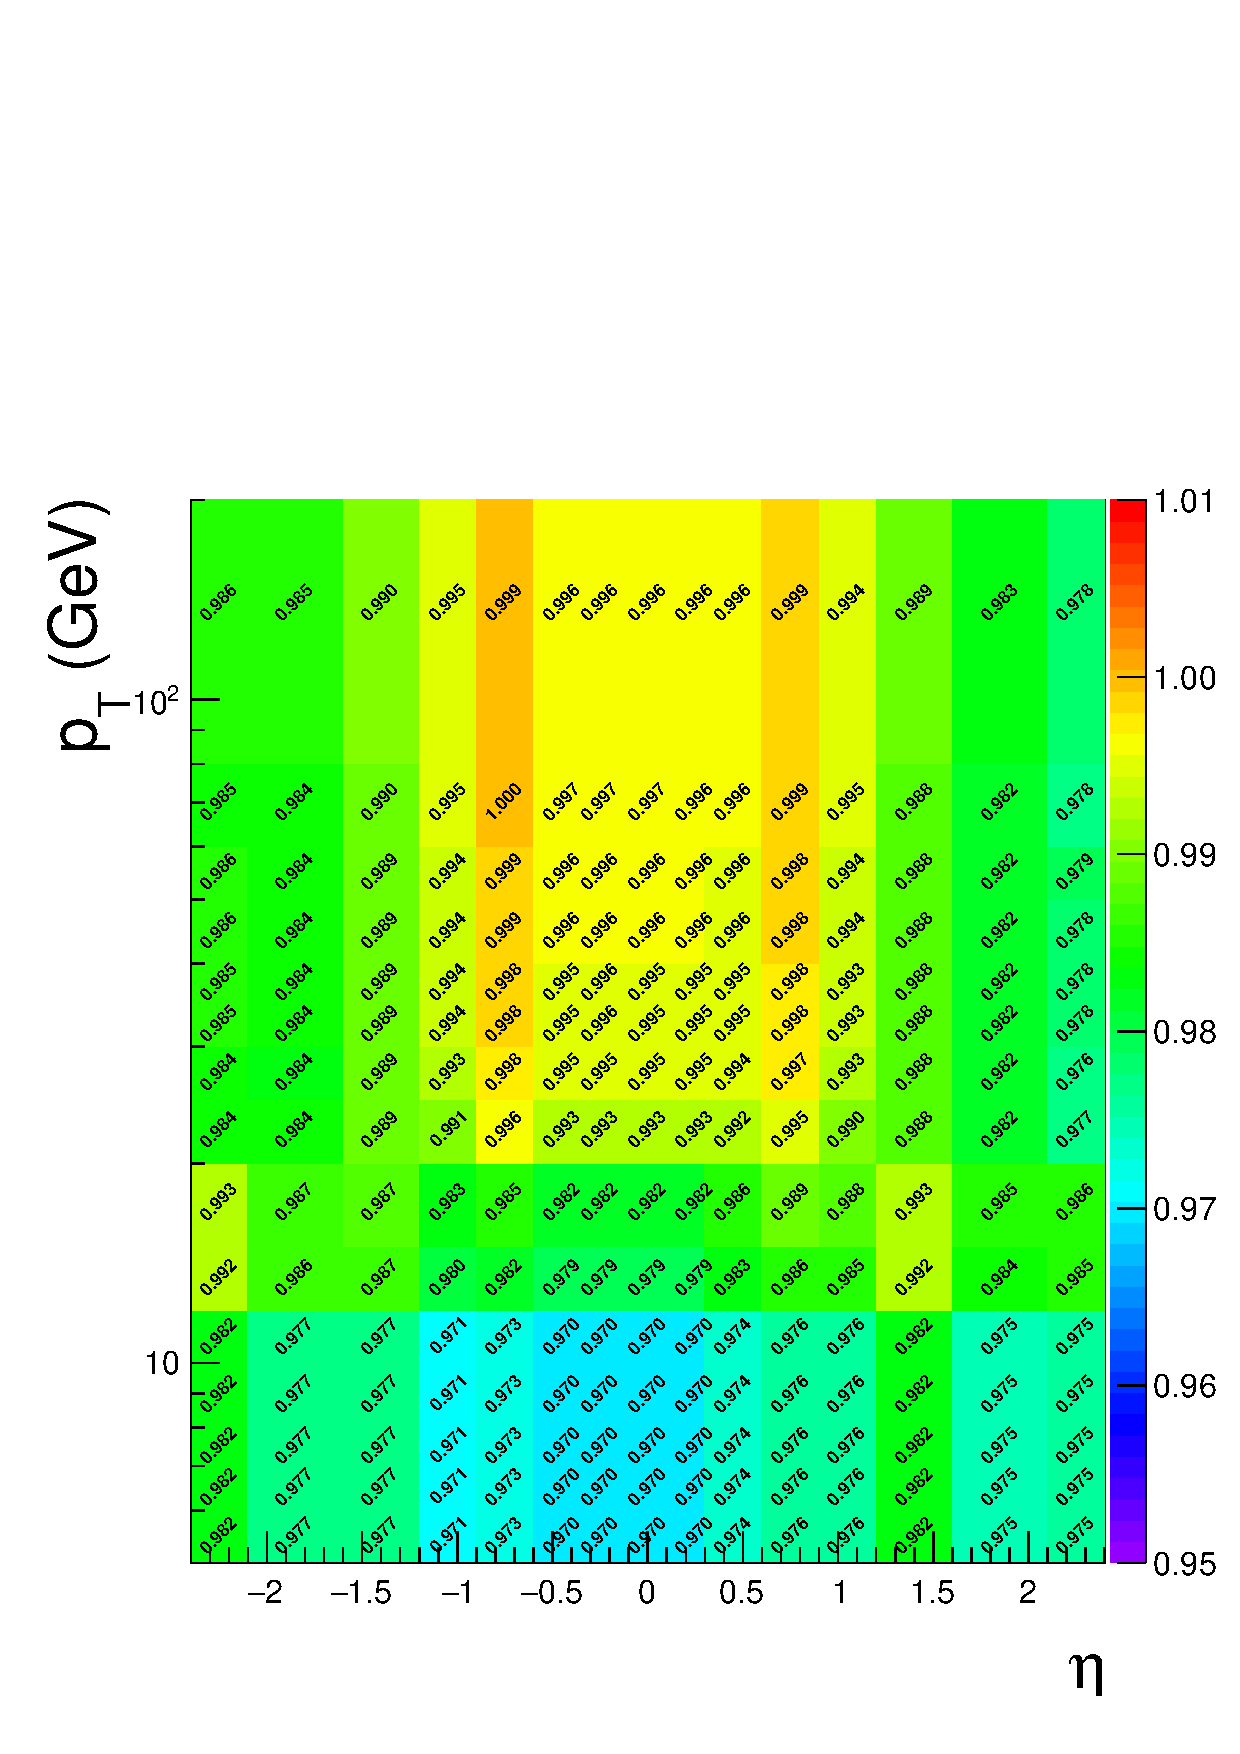
\includegraphics[width=0.45\textwidth]{Figures/Muons/2018UL_SFs.pdf} 
		%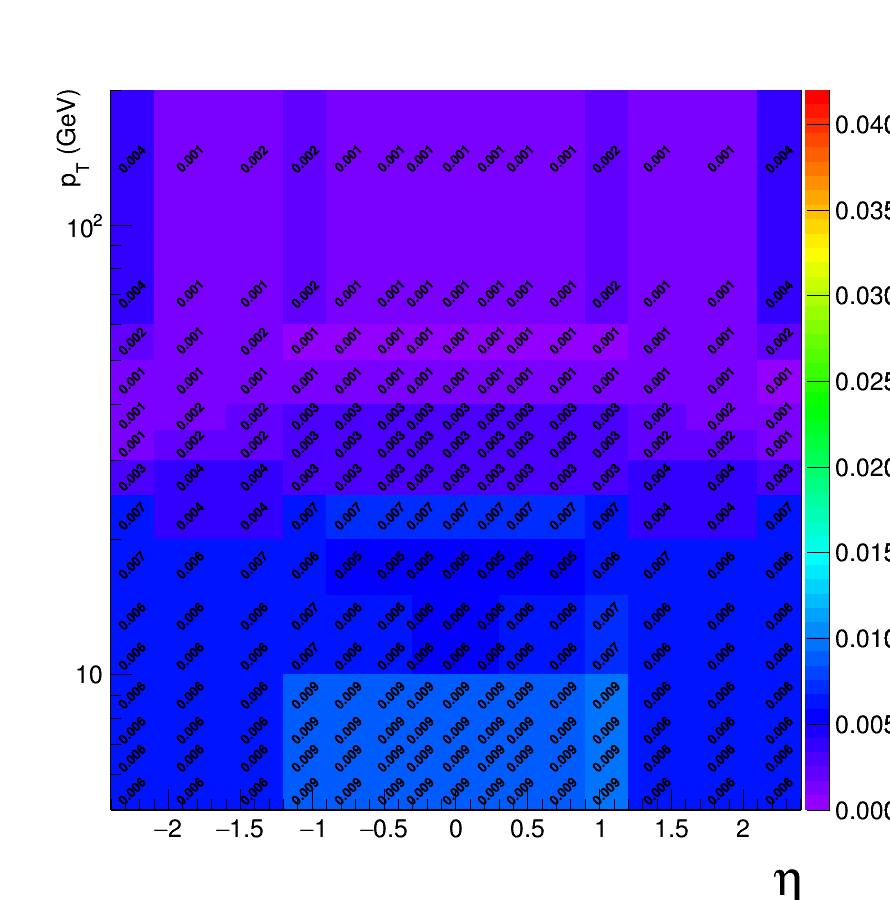
\includegraphics[width=0.45\textwidth]{Figures/Muons/2018_SF_errors_rereco_LooseGT20syst.png}
		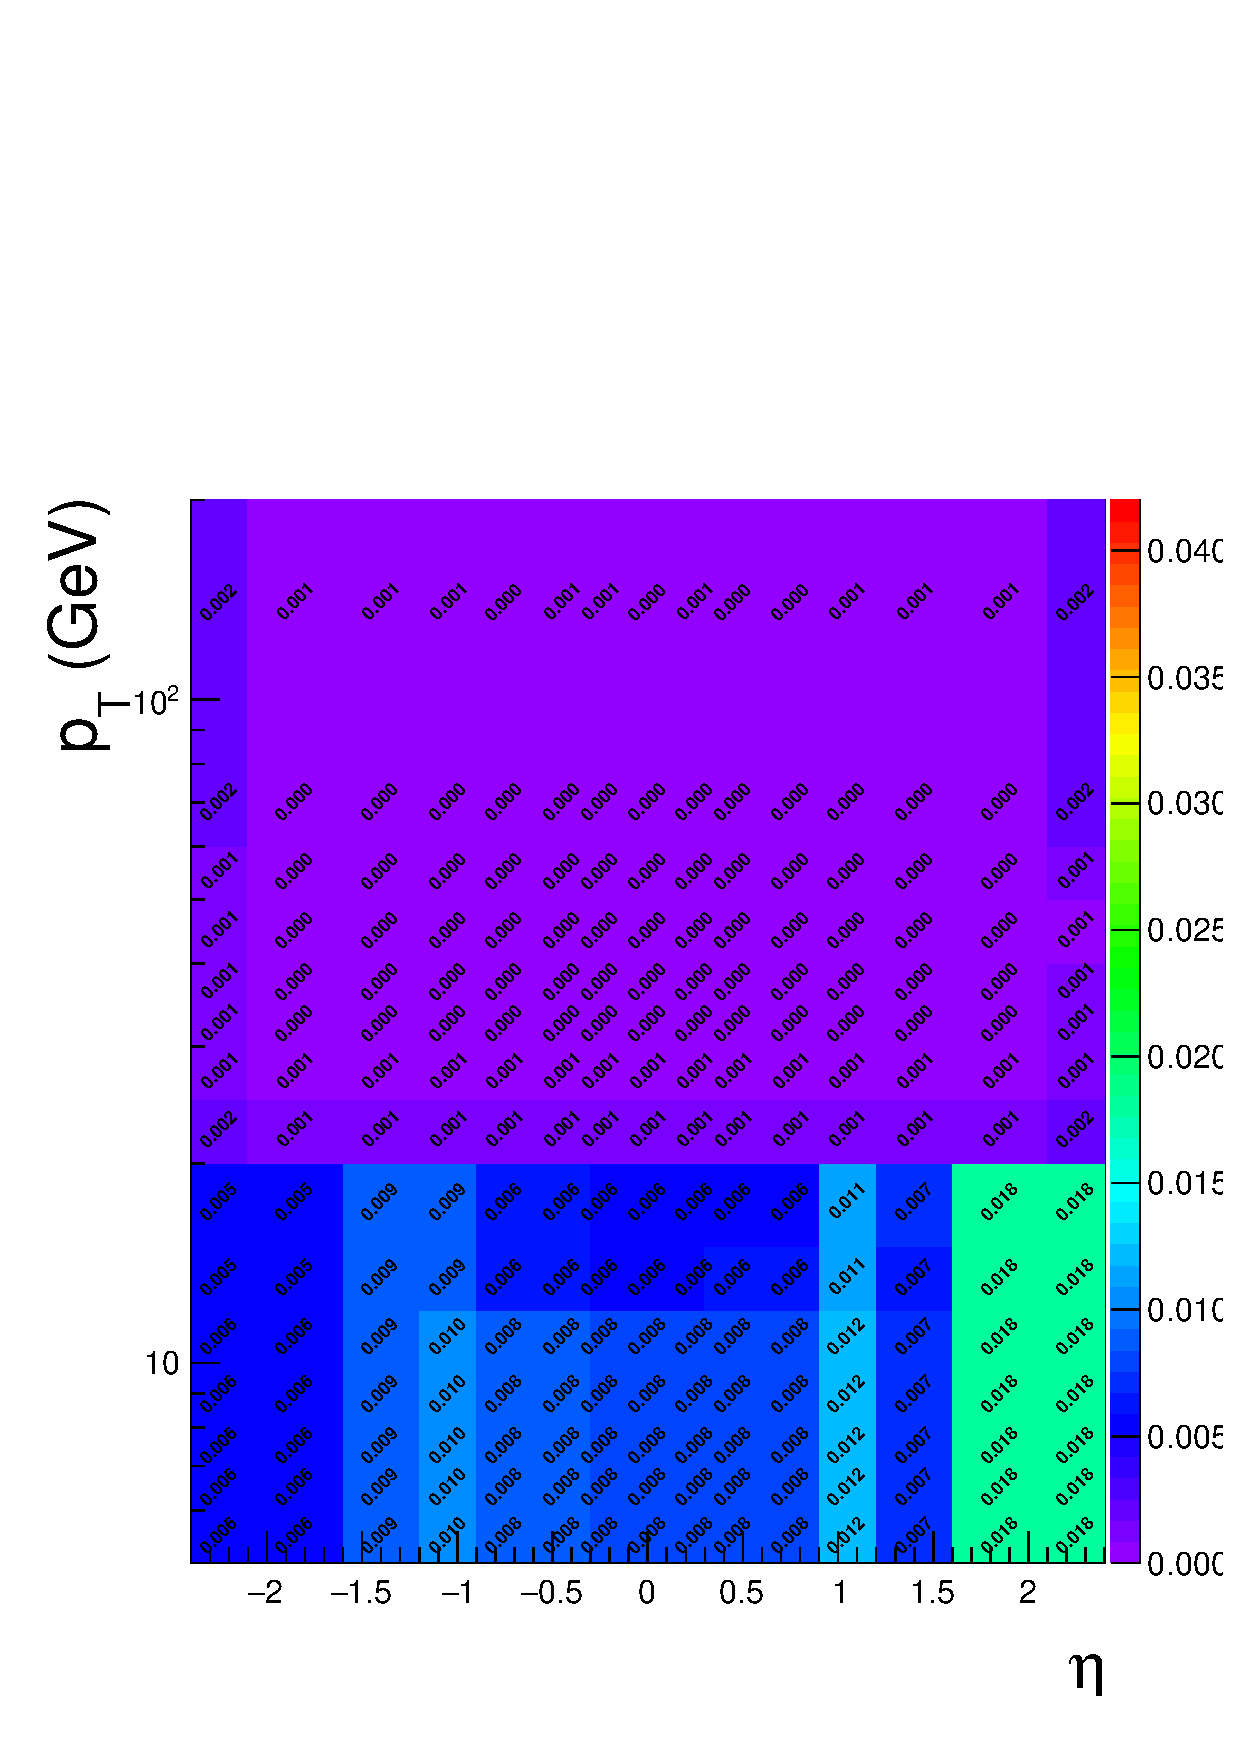
\includegraphics[width=0.45\textwidth]{Figures/Muons/2018UL_SFs_errors.pdf}
    \caption{Left: Overall data to simulation scale factors for muons, as function of \pt and $\eta$. Right: Uncertainties on  data to simulation scale factors for muons, as function of \pt and $\eta$. Results are shown for 2016 (top), 2017 (middle) and 2018 (bottom).}
    \label{fig:MuonIDEff_5}
\end{center}
\end{figure}

